\documentclass[11pt,a4paper,twoside,openright]{report}

\usepackage[pdftex]{graphicx} 	% Biblioteca para uso de figuras
\usepackage{color}

\usepackage[brazil]{babel} 		% Biblioteca para uso da l�ngua Portuguesa
\usepackage[T1]{fontenc} 		% Biblioteca para uso da acentua��o de entrada
\usepackage[latin1]{inputenc} 	% Biblioteca para uso da acentua��o de sa�da

\usepackage{amsthm,amsfonts,amsmath,amssymb}  % Biblioteca para uso de comandos matem�ticos
\usepackage{pslatex}
\usepackage{pstricks,pst-node,color,pst-gantt,pst-coil}
\usepackage{scalefnt}
\usepackage{float} 				% Permite colocar "\begin{figure}[H]" e colocar imagem exatamente onde desejar
\usepackage[hyphens]{url} 		% Para Aceitar URL nas refer�ncias
\usepackage{hyperref}
\usepackage{pdfpages}
\usepackage{gensymb}
\usepackage{eurosym}  			% Pacote para possibilitar o uso do s�mbolo de euro "\euro"
\usepackage{listings}			% Pacote para importa��o de c�digos fonte 

\usepackage{comment}
\usepackage[margin=2.7cm]{geometry}
\renewcommand{\baselinestretch}{1.5}

\setlength{\parskip}{0em}

% Pacote para configurar cabe�alho e rodap�
\usepackage{fancyhdr}
\pagestyle{empty}
\fancyhf{} % clear all header and footer fields

\fancypagestyle{plain}{\pagestyle{fancy}}
\renewcommand{\headrulewidth}{0pt}
\renewcommand{\footrulewidth}{0pt}

\usepackage[titletoc]{appendix} 	% Pacote para organizar ap�ndices 

%------------------------------------- CONFIGURA��ES DE P�GINA --------------------------------------
%\topmargin -2.1cm
%\oddsidemargin 0.5cm 
%\evensidemargin 0.5cm 
%\textwidth 15cm
%\textheight 25.1cm
	
%------------------------------------- IN�CIO DO DOCUMENTO ------------------------------------------
\begin{document}
	
%------------------------------------- INCLUDES -----------------------------------------------------

%------------------------------------- ELEMENTOS PR�-TEXTUAIS ---------------------------------------
%------------------------------------- CONFIGURAÇÕES DE CAPA --------------------------------------
% TODO: Mudar título
\begin{titlepage}
	% Capa Principal
	\begin{center}
		\Huge{UNIVERSIDADE DE SÃO PAULO}\\
		\vspace{0.02\textheight}
		\huge{ESCOLA DE ENGENHARIA DE SÃO CARLOS}\\
		\vspace{0.01\textheight}
		\huge{DEPARTAMENTO DE ENGENHARIA ELÉTRICA}\\
		\vspace{0.2\textheight}
		\huge{\textbf{Mapeamento de ambientes baseado em algoritmos de visão estéreo para VANTs sobre Linux Embarcado}}
		\vspace{0.2\textheight}
	\end{center}
		
		\large
		{
			\begin{flushleft}
			\Large{ \textbf{Autor}: \hspace{1cm} Nícolas dos Santos Rosa}\\
			\Large{ \textbf{Orientador}: \hspace{0.3cm} Prof. Dr. Evandro Luís Linhari Rodrigues }\\
			\end{flushleft}
	
			\begin{center}
				\vspace{0.09\textheight}
				\Large{São Carlos}\\
				\Large{2016}
			\end{center}
		}
	
\end{titlepage}


%------------------------------------- INSERÇÃO PÁGINA EM BRANCO ------------------------------------
\cleardoublepage

%------------------------------------- FOLHA DE ROSTO  ----------------------------------------------
%\vspace{0.01\textheight} 
	\begin{center}
	\vspace{-0.06\textheight}
	%\thispagestyle{empty}
		\Large{\textbf{Nícolas dos Santos Rosa}}\\
		\vspace{0.15\textheight}
		\Huge{\textbf{Mapeamento de ambientes baseado em algoritmos de visão estéreo para VANTs sobre Linux Embarcado}} 
		\vspace{0.08\textheight}
	\end{center}
		
		\large
		{
			\begin{flushright}
			\Large{Trabalho de Conclusão de Curso apresentado} \hspace{1cm}\\
			\Large{à Escola de Engenharia de São Carlos, da}\\
			\Large{Universidade de São Paulo}\\
			\vspace{0.05\textheight}
			\Large{Curso de Engenharia Elétrica}\\
			\vspace{0.05\textheight}
			\Large{ORIENTADOR: Prof. Evandro Luís Linhari Rodrigues}\\
			\end{flushright}
	
			\begin{center}
				\vspace{0.15\textheight}
				\Large{São Carlos}\\
				\Large{2016}
			\end{center}
		}



%------------------------------------- FICHA CATALOGRÁFICA ------------------------------------------
\newpage

Página com a ficha catalográfica (em página par).

%ficha catalografica no verso
%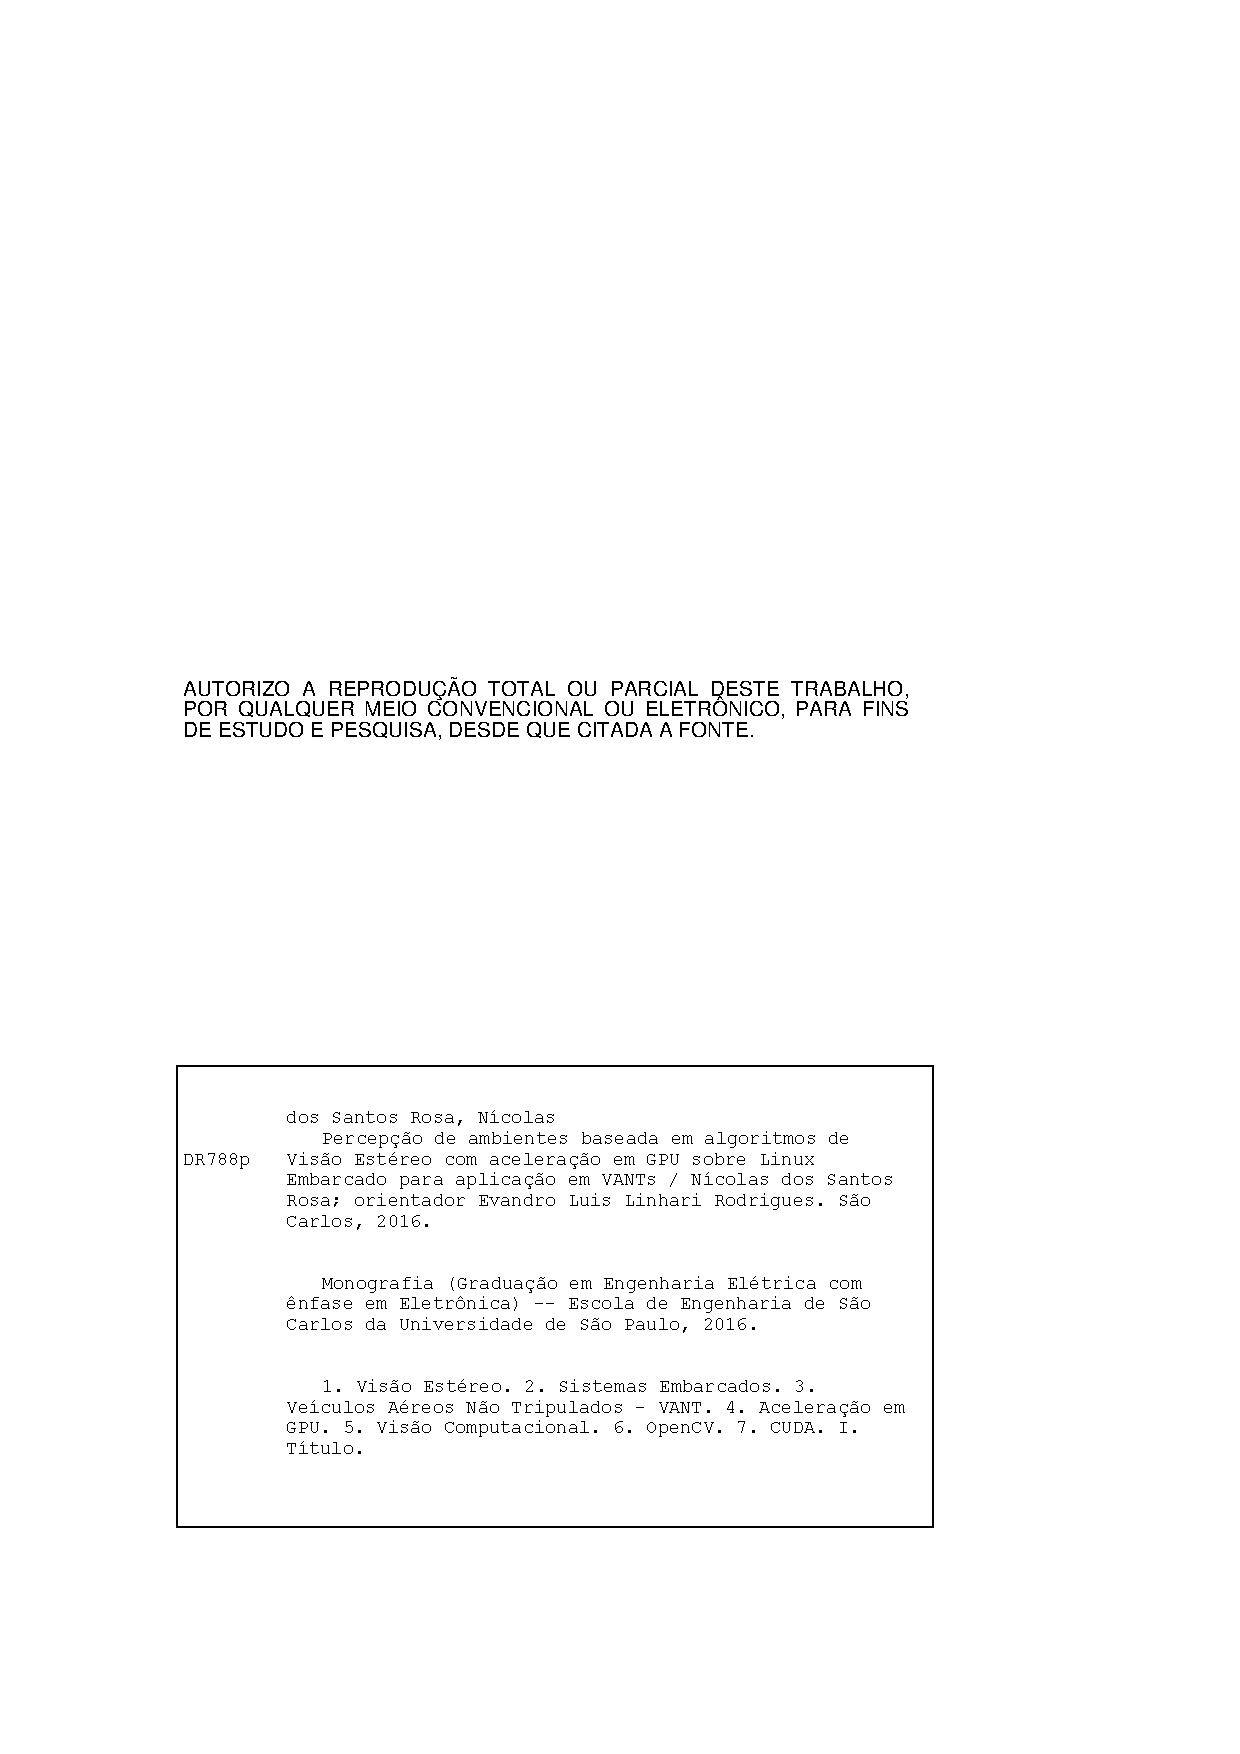
\includepdf{./Resources/ficha_catalografica.pdf}

%------------------------------------- Folha de aprovação--------------------------------------------
\newpage

página com a folha de aprovação (página ímpar). \cleardoublepage

\begin{comment}
\begin{figure}[H]
	\centering
	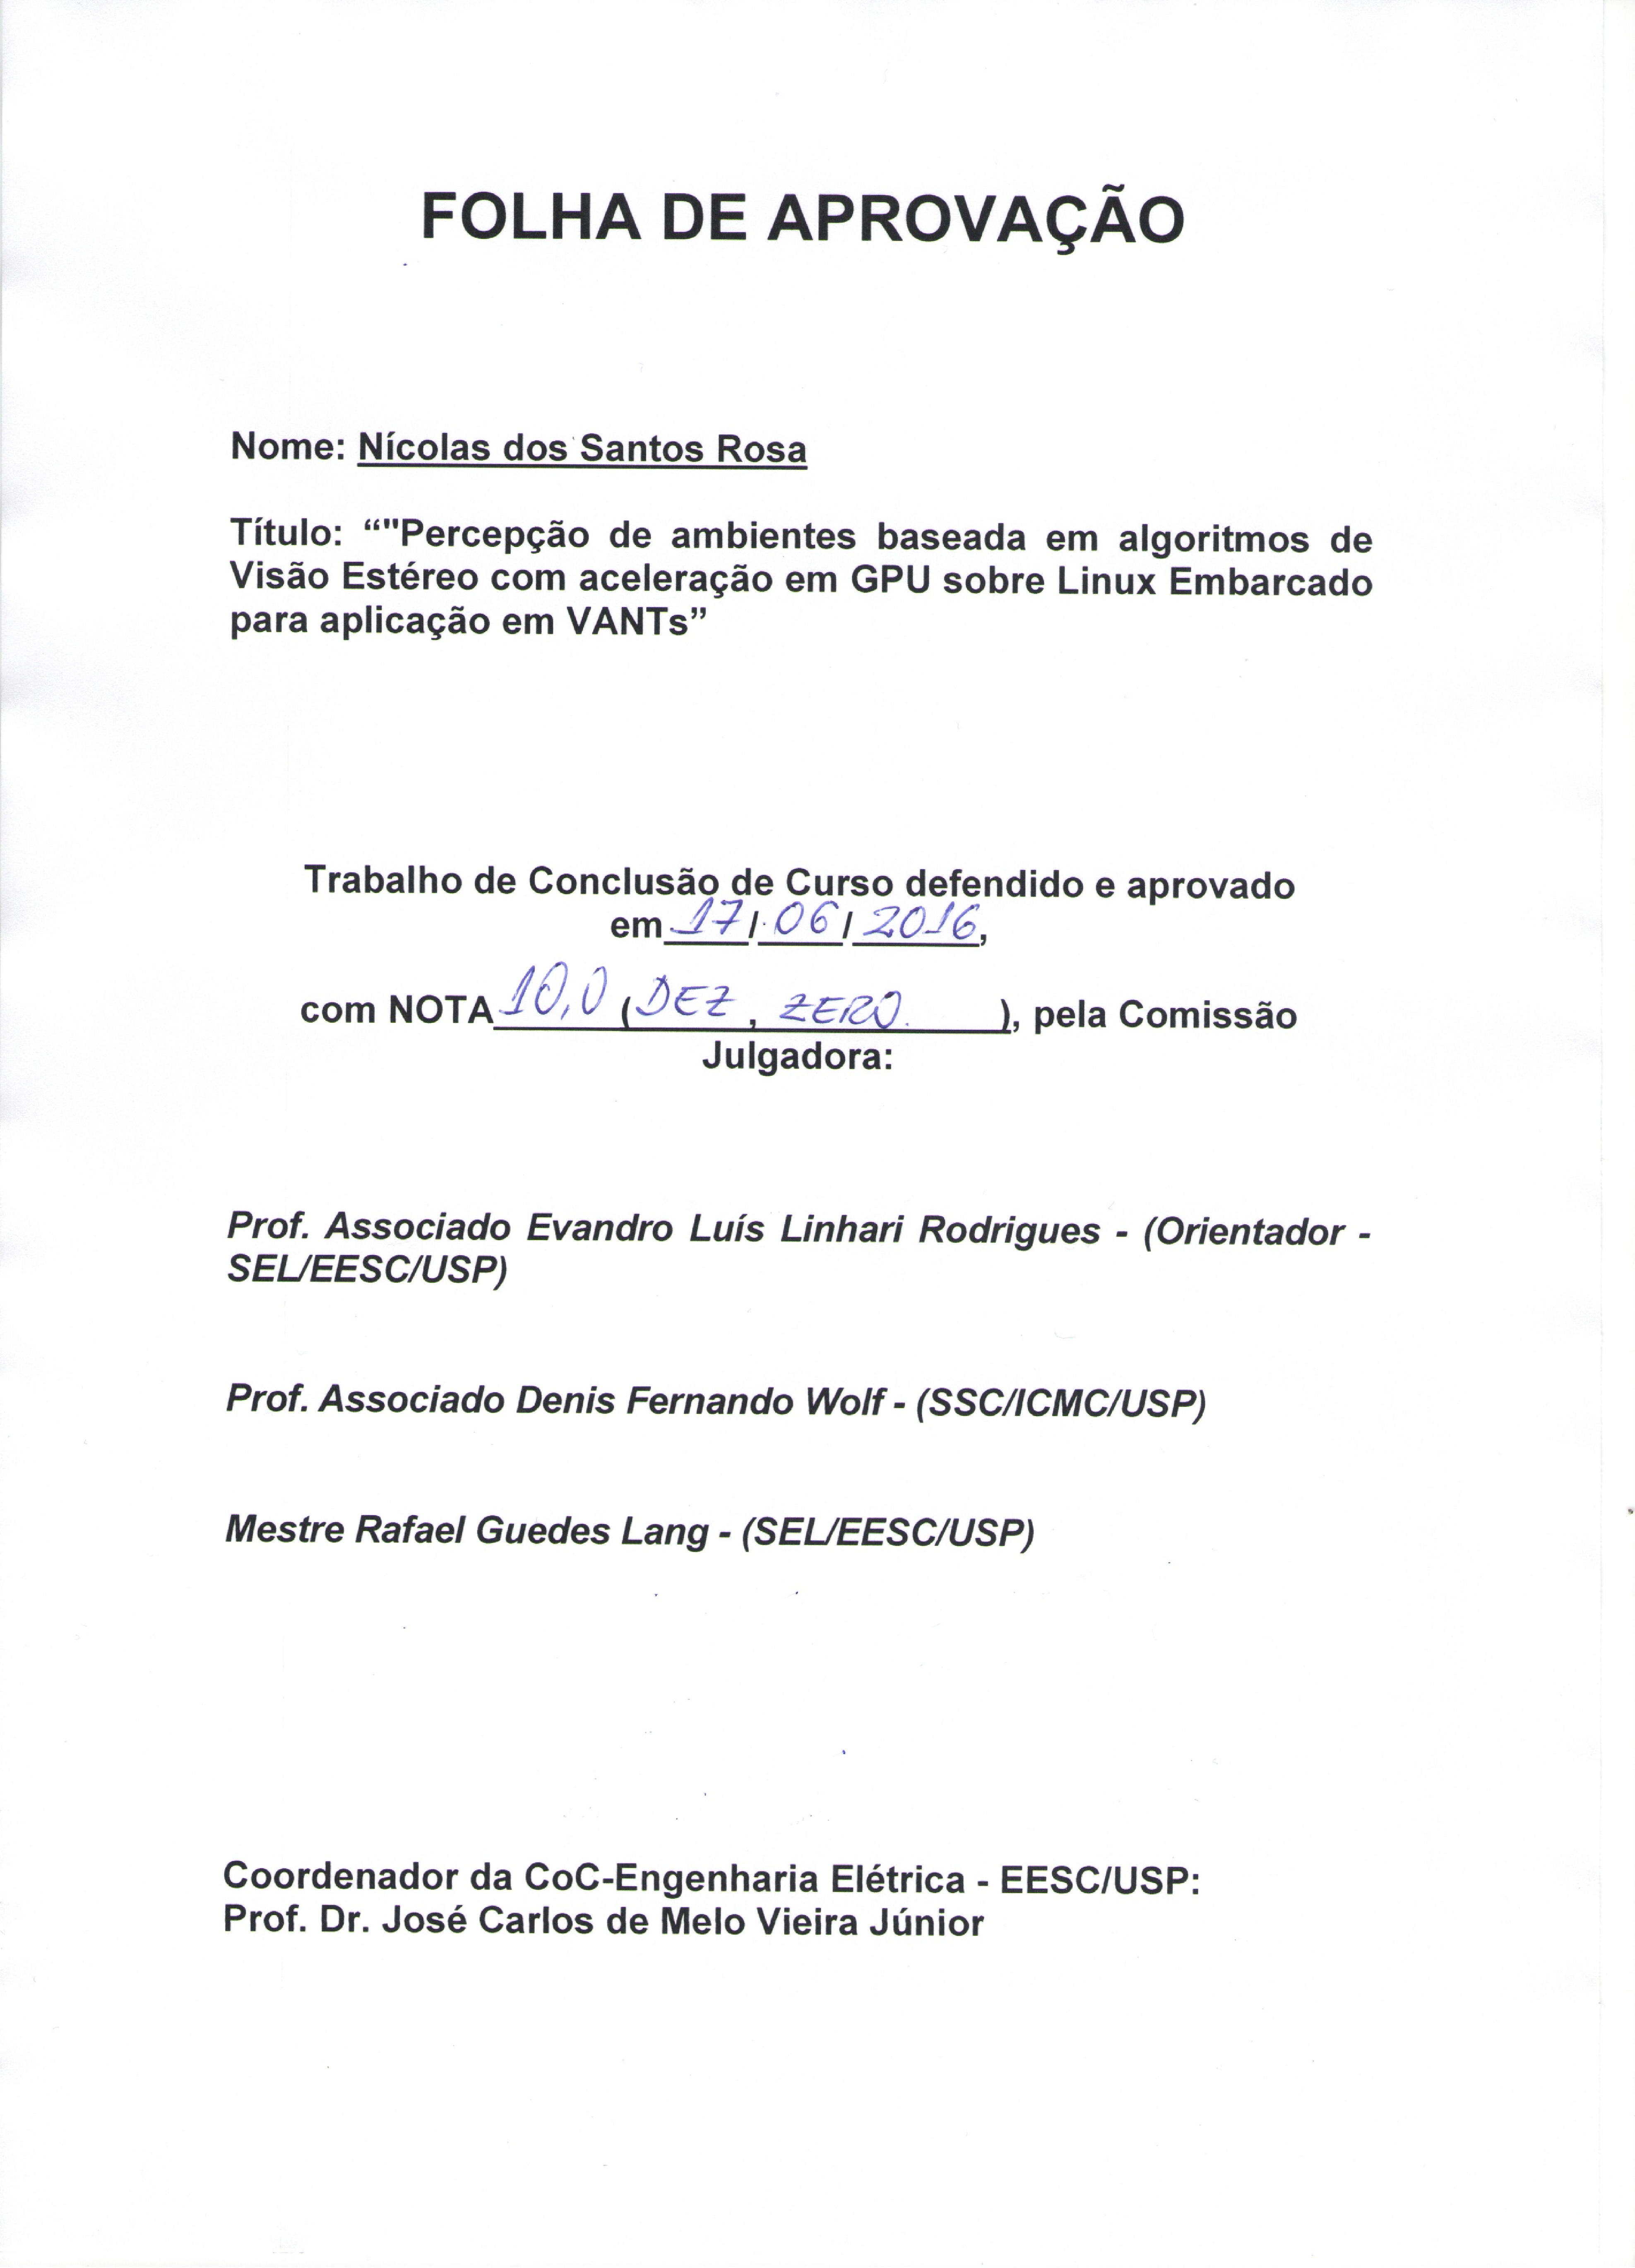
\includegraphics[scale=0.3]{./Resources/aprovacao.jpg}
	\caption{Fluxo de comunicação entre os principais componentes.}
	\label{Aprovacao}
\end{figure}
\cleardoublepage
\end{comment}
%------------------------------------- Dedicatória --------------------------------------------------
\vspace{0.11\textheight} 
\begin{center}
\textbf{\Huge{Dedicatória}}
\end{center}
\vspace{0.05\textheight}

Este trabalho de conclusão de curso é dedicado à minha mãe, ao meu pai, à minha irmã, aos meus padrinhos e a toda minha família.

\begin{flushright}
Nícolas dos Santos Rosa.
\end{flushright}

%------------------------------------- INSERÇÃO PÁGINA EM BRANCO ------------------------------------
\cleardoublepage

%------------------------------------- Agradecimentos -----------------------------------------------
\vspace{0.11\textheight} 

\begin{center}
\textbf{\Huge{Agradecimentos}}
\end{center}

\vspace{0.05\textheight}

Primeiramente, agradeço a Deus por propiciar saúde e felicidade a todos aqueles que me rodeiam.

À minha família: à minha mãe, Valdenilce, pela ferrenha dedicação em mostrar a mim e a minha irmã a importância da educação para nossa formação pessoal; ao meu pai, Francisco, por fazer o possível e o impossível para sustentar nossa família e por possibilitar condições para que me tornasse engenheiro; à minha irmã, Natália, pelo suporte e carinho e por ser a dupla perfeita para atazanar nossos pais; às minhas tias, Elisabeth, Vera Lúcia e Maria Regina, por serem minhas segundas mães, visto o tamanho do suporte, preocupação, e apreço dado. 

Ao meu orientador, Prof. Evandro Luís Linhari Rodrigues, pelo apoio para o desenvolvimento deste trabalho e por despertar meu interesse em sistemas embarcados, confirmando ainda mais minha paixão pelo meu curso.  

Aos meus orientadores de iniciação científica, Prof. Dr. Cláudio F. M. Toledo e Márcio S. Arantes, por introduzir-me ao âmbito da pesquisa acadêmica. Aos membros do SARLab: ao Prof. Dr. Samir Rawashdeh por ser o idealizador deste trabalho e por oferecer a oportunidade de desenvolvê-lo; a Benjamin Dale e a Miguel Rocha Jr., pelo companheirismo e por sempre estarem sempre de prontidão.

Aos meus amigos de curso, pelos ótimos momentos que vivemos juntos nestes anos, especialmente, Alexandre B. Moretti, Leonardo B. Farçoni, Plínio G. B. Ferreira, Marília L. Dourado,  Jéssica B. da Vida, Pedro Arantes, Augusto Martins, Gustavo Oliveira, Aline Midori, Vitor Martins, Anderson M. Tsai, Victor Morini, João F. Corsini, Caio Martins e a todos os outros amigos. 

Aos membros do grupo extracurricular Warthog Robotics, por partilhar um interesse em comum e pelas incontáveis horas de dedicação gastas no laboratório.

Por fim, agradeço a todos os envolvidos no desenvolvimento deste trabalho.

\begin{flushright}
Nícolas dos Santos Rosa.
\end{flushright}


%------------------------------------- INSERÇÃO PÁGINA EM BRANCO ------------------------------------
\cleardoublepage

%------------------------------------- EPÍGRAFE -----------------------------------------------------
\
\vspace{0.76\textheight} 

\begin{flushright}

\textit{"O dinheiro faz homens ricos, o conhecimento faz homens }

\textit{sábios e a humildade faz grandes homens."}

Mahatma Gandhi

\textit{"You can't put a limit on anything. The more you dream, the farther you get."}

Michael Phelps

\textit{"Se eu vi mais longe, foi por estar sobre ombros de gigantes."}

Isaac Newton

\end{flushright}


%------------------------------------- INSERÇÃO PÁGINA EM BRANCO ------------------------------------
\cleardoublepage

%------------------------------------- Resumo - Português -------------------------------------------
\vspace{0.11\textheight} 

\begin{center}
\textbf{\Huge{Resumo}}
\end{center}

\vspace{0.05\textheight}

Rosa, Nícolas \textbf{Mapeamento de ambientes baseado em algoritmos de visão estéreo para VANTs sobre Linux Embarcado}. Trabalho de Conclusão de Curso -- Escola de Engenharia de São Carlos, Universidade de São Paulo, 2016.

\vspace{0.05\textheight}

Atualmente, veículos aéreos não tripulados (VANT) vêm tornando-se um assunto recorrente no âmbito científico. Estes veículos, devido a sua mobilidade e inteligência artificial, vêm sendo adaptados para a atuação em diferentes ambientes, desempenhando assim diversas atividades que vão desde aplicações militares, agronômicas, espaciais, cinematográficas, entre outras. Entretanto, essa atuação só não é mais ampla devido a problemas relacionados ao reconhecimento do ambiente ao seu redor e detecção de objetos e obstáculos. Neste trabalho, estudou-se a utilização de visão estéreo em sistemas embarcados para mapeamento de ambientes e obstáculos ameacem a locomoção do veículo autônomo. Os métodos estéreo mais conhecidos pela literatura, BM (\textit{Block Matching}) e SGBM (\textit{Semi-Global Block Matching}), foram implementados e também foi desenvolvido uma interface que facilite a extração de informações e a comparação de performance destes métodos. Após análise, o algoritmo mais robusto para a aplicação em veículos aéreos foi o método BM para ambas as plataformas, BBB e \textit{Jetson TK1}. Visto que a \textit{Jetson TK1} permite a aceleração em hardware do método BM, foi possível implementar o método BMGPU (\textit{Block Matching with GPU Acceleration}) fornecido pelo OpenCV nesta plataforma. Por fim, os algoritmos utilizados permitiram que as distâncias de objetos próximos ao veículo móvel pudessem ser estimadas.

\vspace{0.05\textheight}

Palavras-Chave: Visão estéreo, Detecção de Obstáculos, Sistemas Embarcados, Veículos Aéreos Não Tripulados - VANT, Visão Computacional, OpenCV, Aceleração em GPU, CUDA.


%------------------------------------- INSERÇÃO PÁGINA EM BRANCO ------------------------------------ 
\cleardoublepage


%------------------------------------- Resumo - Inglês ----------------------------------------------
\vspace{0.11\textheight} 

\begin{center}
\textbf{\Huge{Abstract}}
\end{center}

\vspace{0.05\textheight}

Rosa, Nícolas \textbf{Environment Mapping based on Stereo Vision algorithms for UAVs on Embedded Linux}. Completion of course work -- São Carlos School of Engineering, University of São Paulo, 2016.

\vspace{0.05\textheight}

Currently, Unmanned Aerial Vehicles (UAV) are becoming a recurring theme in the scientific realm. These vehicles, because of their mobility and artificial intelligence, have been adapted to perform in different environments, thus performing various activities ranging from
military applications, agronomic, spacial, cinematographic, among others. However, this performance is not wider due to  problems related to the recognition of the surrounding environment and the detection objects and obstacles.In this work, it was studied the use of stereoscopic vision in embedded systems for environment mapping and obstacles that threaten the mobility of the autonomous vehicle. The most well known stereo methods in the literature, BM (\textit{Block Matching}) and SGBM (\textit{Semi-Global Block Matching}) were implement and was developed a graphical user interface, which facilitates the extraction of the information and comparing performance of these methods. After analysis, the most robust algorithm for use in aerial vehicles was the BM method for both platforms, BBB and \textit{Jetson TK1}. Since the \textit{Jetson TK1} allows hardware acceleration of the method BM, it was possible to implement the method BMGPU (\textit{Block Matching with GPU Acceleration}) provided by OpenCV on this platform. Finally, the used algorithms allowed the distances of obstacles near the moving vehicle could be estimated.

\vspace{0.05\textheight}

Keywords: Stereo Vision, Obstacle Detection, Embedded Systems, Unmanned aerial Vehicle - UAV, Computational Vision, OpenCV, GPU Acceleration, CUDA.


%------------------------------------- INSERÇÃO PÁGINA EM BRANCO ------------------------------------
\cleardoublepage

%------------------------------------- CONFIGURAÇÕES DOS ÍNDICES ------------------------------------
%\clearpage
%\thispagestyle{empty}
\listoffigures % Índice de Figuras

\listoftables % Índice de Tabelas

%------------------------------------- INSERÇÃO PÁGINA EM BRANCO ------------------------------------ 
\cleardoublepage

%------------------------------------- LISTA DE ABREVIATURAS ----------------------------------------
\vspace{0.11\textheight} 

\textbf{\Huge{Siglas}}

\vspace{0.05\textheight}

\begin{tabbing}
\hspace*{0.5cm}\=\hspace{2.5cm}\= \kill

% Lista de Abreviaturas
\> AAVC		\> \textit{Autonomous Aerial Vehicle Competition}									\\
\> AFRL		\> \textit{Air Force Research Laboratory} - Laboratório de pesquisas da Força Aérea Americana 				\\ 
\> ALU		\> \textit{Arithmetic Logic Unit} - Unidade Lógica e Aritmética				 				\\ 
\> ANAC		\> Agência Nacional de Aviação Civil 											\\
\> API		\> \textit{Application Programming Interface} - Interface de Programação de Aplicações					\\
\> AUV		\> \textit{Autonomous Underwater Vehicle} - Veículo Submarinos Autônomo	 						\\
\> BBB		\> \textit{BeagleBone Black}	 											\\
\> BM		\> \textit{Block Matching} - Método Estéreo Local	 								\\
\> BMGPU	\> \textit{Block Matching with GPU Acceleration} - 									\\
\>		\> Método Estéreo Local com Aceleração de GPU										\\
\> CPU		\> \textit{Central Processing Unit} - Unidade central de Processamento							\\
\> CUDA		\> \textit{Compute Unified Device Architecture} - Plataforma de computação paralela					\\
\> DECEA	\> Departamento de Controle do Espaço Aéreo										\\
\> FAA	 	\> \textit{Federal Aviation Administration} - Administração Federal de Aviação						\\
\> FPGA  	\> \textit{Field-programmable gate array} - Arranjo de Portas Programável em Campo					\\
\> FPS  	\> \textit{Frames per Second} - Quadros por Segundo									\\
\> GUI 	 	\> \textit{Graphical User Interface} - Interface gráfica do usuário							\\
\> GPU 	 	\> \textit{Graphics Processing Unit} - Unidade de Processamento Gráfico							\\
\> GPGPU 	\> \textit{General Purpose Graphics Processing Unit} -  								\\
\>		\> Unidade de Processamento Gráfico de Propósito Geral									\\
\> GPS 	 	\> \textit{Global Positioning System} - Sistema de Posicionamento Global						\\
\> LIDAR 	\> \textit{LIght Detection And Ranging}											\\
\> LMR 	 	\> Laboratório de Robótica Móvel											\\
\> MAVS  	\> \textit{Micro Air Vehicle} - Micro Veículo Aéreo									\\
\> MIT 	 	\> \textit{Massachusetts Institute of Technology}									\\
\> OACI  	\> Organização de Aviação Civil Internacional 										\\
\> RPA 	 	\> \textit{Remotely Piloted Aircraft} - Aeronave Remotamente Pilotada							\\
\> RTOS	 	\> \textit{Real-Time Operating System} - Sistema Operacional em Tempo Real						\\
\> SGBM  	\> \textit{Semi-Global Block Matching} - Método Estéreo Semi-global							\\
\> SIMD  	\> \textit{Single Instruction, Multiple Data}										\\
\> SLAM  	\> \textit{Simultaneous Localization and Mapping} - Localização e Mapeamento Simultâneo					\\
\> UAV/VANT 	\> \textit{Unmanned aerial vehicle} - Veículo Aéreo não tripulados 							\\

\end{tabbing}
\cleardoublepage
%------------------------------------- CONFIGURAÇÕES DOS ÍNDICES ------------------------------------ 
%\usepackage{fancyhdr}
\pagestyle{fancy}
\fancyhf{} % clear all header and footer fields
\fancyhead[RO, LE] {\thepage}

\fancypagestyle{plain}{\pagestyle{fancy}}

\tableofcontents % Índice Geral


%------------------------------------- Adi��o dos Cap�tulos -----------------------------------------	
\chapter{Introdu��o}
\label{Introducao}

A pesquisa em VANTs -- Ve�culos A�reos n�o Tripulado vem se tornando um assunto recorrente no �mbito cient�fico. A real motiva��o para seu desenvolvimento levanta diversas quest�es �ticas e legais, visto que foram inicialmente motivados para fins militares. Por outro lado, esse tipo de plataforma tamb�m possui aplica��es tais como: cultivo e pulveriza��o de culturas, produ��o cinematogr�fica, opera��es de busca e salvamento, inspe��o de linhas el�tricas de alta tens�o, entrega de mercadorias e encomendas.

A navega��o de um micro ve�culo a�reo em espa�o confinado � um desafio significante. Atualmente, a navega��o aut�noma enfrenta o problema de localiza��o e mapeamento simult�neo, mais conhecido como SLAM (Simultaneous Localization and Mapping) \cite{Dissanayake2001}. SLAM apresenta quatro etapas: Mapeamento, Percep��o, Localiza��o e Modelagem. A complexidade deste problema encontra-se no fato de que o ve�culo necessita navegar em um espa�o desconhecido, extrair caracter�sticas importantes do ambiente, construir um mapa com os dados obtidos e simultaneamente localizar-se dentro deste. O sensoriamento pode ser realizado tanto por Vis�o computacional ou por sensores �pticos. 

A proposta deste Trabalho de conclus�o de Curso � auxiliar o primeiro passo de Mapeamento de ambientes atrav�s de vis�o estereosc�pica. Este trabalho, � motivado a tentativa de reproduzir-se o desafio proposto pela Autonomous Aerial Vehicle Competition (AAVC)\cite{AAVC}, competi��o organizada pelo Laborat�rio de Pesquisas da Forca A�rea Americana (AFRL) e sediada em Dayton-OH. Esta competi��o incentiva o estudo de ve�culos a�reos aut�nomos, convidando diversas universidades a compartilhar seus avan�os nesta �rea de pesquisa. O competidor � motivado a adaptar um modelo de quadric�ptero 3DRobotics�, assim este ve�culo precisa cumprir um certo percurso com caixas como obst�culos,detectar e reportar � esta��o base a posi��o de um objeto.

O processo de desenvolvimento do ve�culo consiste em quatro passos: estrutura, circuito, controle e navega��o. Os dois primeiros itens comp�em o hardware, o qual estabelece as conex�es f�sicas necess�rias para integrar os sistemas de alimenta��o, comunica��o e controle. A parte de software engloba o desenvolvimento de algoritmos visando o controle e navega��o, mais especificamente o desenvolvimento do c�digo para Vis�o Est�reo (Stereo Vision) \cite{Lemaire2007}, planejamento de caminho (Path Planning) e arquitetura de m�quina de estados (Decision Making).

Um sistema aut�nomo tamb�m implica o processamento de imagens ser embarcado, isto �, o processamento para a navega��o do ve�culo ser realizada \textit{On-line}. Deste modo, as plataformas de desenvolvimento BeagleBone Black e Nvidia jetson TK1 ser�o analisadas e avaliadas com rela��o performance ao executar o algoritmo desenvolvido \cite{Shah2014}. 

\textcolor{red}{-----------------------------------------------------------------------------------------------}

Refer�ncia \cite{referencia1}.

Outra refer�ncia para a bibliografia \cite{referencia2}.

Refer�ncia para a figura \ref{logo}.

 \begin{figure}[H]
 	\centering
 	
\includegraphics[scale=0.35]{./Resources/latex-logo.png}
 	\caption{Logo do LaTeX.}
 	\label{logo}
 \end{figure}


% % % % % % % % % % % % % % % % % % % % % % % % % % % % % % % % % % % % % % % % % % % % % % % % % % %
\section{Objetivos}
\textcolor{red}{\textbf{Dica:} Apresente "somente" os objetivos - podem ser gerais e/ou espec�ficos}

\textcolor{red}{
\begin{enumerate}
	\item Desenvolvimento de um algoritmo de controle para ve�culo a�reo aut�nomo
	\item Estudo e aplica��o do algoritmo de localiza��o e mapeamento simult�neo baseado em Vis�o (Vision-based SLAM)
	\item Desenvolvimento de c�digo da Vis�o do Quadric�ptero para Linux Embarcado
	\item Utiliza��o da Plataforma ROS (Robot Operating System)
	\item Reproduzir o desafio proposto pela AAVC Competition	
\end{enumerate}
}
% % % % % % % % % % % % % % % % % % % % % % % % % % % % % % % % % % % % % % % % % % % % % % % % % % %
\section{Justificativa}
\textcolor{red}{\textbf{Dica:} Explana��o sobre porque o trabalho se
justifica e quais os pontos de relev�ncia do mesmo}

% % % % % % % % % % % % % % % % % % % % % % % % % % % % % % % % % % % % % % % % % % % % % % % % % % %
\section{Motiva��o}
\textcolor{red}{\textbf{Dica:} Um pequeno texto sobre o que motivou o desenvolvimento do
Trabalho}

% % % % % % % % % % % % % % % % % % % % % % % % % % % % % % % % % % % % % % % % % % % % % % % % % % %
\section{Organiza��o do trabalho}
\textcolor{red}{\textbf{Dica:} Apresente o que tem em cada cap�tulo.}































%\chapter{Especificação do Projeto}
%\label{Especificacao}
%
%Especificação do projeto.
%
%
%
%%------------------------------------ Seção 1 --------------------------------------------------------
%\section{Seção 1}
%
%Seção dentro de um capítulo. 
%
%
%
%%------------------------------------ Seção 2 --------------------------------------------------------
%\section{Seção 2}
%
%Outra seção dentro do capítulo.
%

%-----------------------------------------------------------------------------------------------------------------------------------------------------------------------------------------------
% Embasamento Teórico ou Fundamentação Teórica: revisão da literatura dos tópicos que sustentam a ciência e o conhecimento, relativos aos objetivos e aos métodos escolhidos para o desenvolvimento do trabalho.
% Itens como Considerações Iniciais e Finais não são obrigatórios, mas completam muito bem qualquer capítulo.
\chapter{Fundamentos Teóricos}
\label{Revisão Bibliográfica}

A visão estéreo possibilita boa identificação de um espaço tridimensional, visto que sua estrutura permite a triangulação de pontos chaves, assim determinando o seu correto posicionamento. Deste modo, compreende-se o porquê deste sistema visual ser amplamente difundido na evolução humana e animal. Em visão computacional, deseja-se emular os sistemas de visão mais eficientes para identificação de objetos e reconhecimento de ambientes. Este processo pode ser realizado  computacionalmente, porém com alguns conceitos como Triangulação, Geometria Epipolar, Calibração e Retificação e Correspondência Estéreo. Estes conceitos encontram-se apresentados nas próximas seções.


%-----------------------------------------------------------------------------------------------------------------------------------------------------------------------------------------------
\section{Visão Estéreo - \textit{Stereo Vision}}
\subsection{Triangulação - \textit{Triangulation}}

Idealmente, a triangulação de um ponto P de coordenadas globais $(X,Y,Z)$ pode ser realizada caso tenha-se uma estrutura estéreo, cujas lentes não apresentem distorção e estejam perfeitamente alinhadas. Deste modo, matematicamente, é possível abstrair os sensores das câmeras como dois planos coplanares entre si. Nessas condições, tem-se que os eixos ópticos das câmeras são paralelos. O eixo óptico, também conhecido como raio principal, é a reta que intercepta o ponto de centro de projeção ${O}$ e o ponto principal da lente ${c}$. Assumindo que as câmeras sejam exatamente iguais e alinhadas, tem-se que os pontos focais da câmera esquerda e da câmera direita são iguais ${f_l = f_r}$ e os pontos principais ${c^{left}_x}$ e  ${c^{right}_x}$ apresentam as mesmas coordenadas \cite{Bradski2008}. A figura \ref{stereo_image_geometric_model} ilustra a representação do modelo idealizado de um sistema estéreo.

\begin{figure}[H]
 	\centering
 	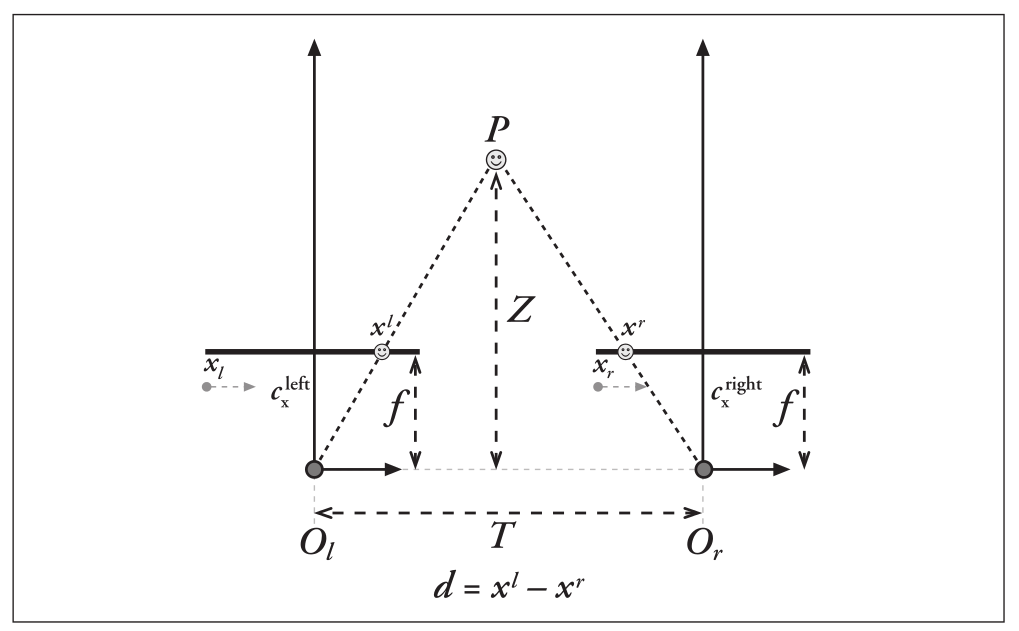
\includegraphics[scale=0.35]{./Resources/bradski/stereo_image_geometric_model.png}
 	\caption{Modelo Idealizado de um sistema de visão estéreo. Imagem retirada de \cite{Bradski2008}}
 	\label{stereo_image_geometric_model}
\end{figure}

A distância presente entre os pontos $x^l$ e $x^r$ é dada pela equação $d = x^l - x^r$, o valor de $d$ é comumente também de chamado de disparidade. Caso os pontos $x^l$ e $x^r$, a distância focal $f$, a distância entre os centros das câmeras $(T,baseline)$ sejam conhecidos é possível determinar a distância entre o ponto P à base das câmeras $(Z)$. Por meio de semelhanças de triângulos, é possível estabelecer uma relação entre os triângulos $O_lPO_r$ e $x^lPx^r$, a qual está apresentada na equação \ref{triangle_similarity}.

\begin{equation}
\label{triangle_similarity}
\frac{T - (x^l-x^r)}{Z-T} = \frac{T}{Z} \Rightarrow Z = \frac{fT}{(x^l-x^r)} = \frac{fT}{d}
\end{equation}


%-----------------------------------------------------------------------------------------------------------------------------------------------------------------------------------------------
\subsection{Geometria epipolar - \textit{Epipolar Geometry}}

Geometria epipolar corresponde à estrutura básica de um sistema estéreo, na qual leva em consideração os modelos \textit{pinhole} de ambas câmeras utilizadas e encontra-se ilustrada pela figura \ref{geometry_epipolar}. 

\begin{figure}[H]
 	\centering
 	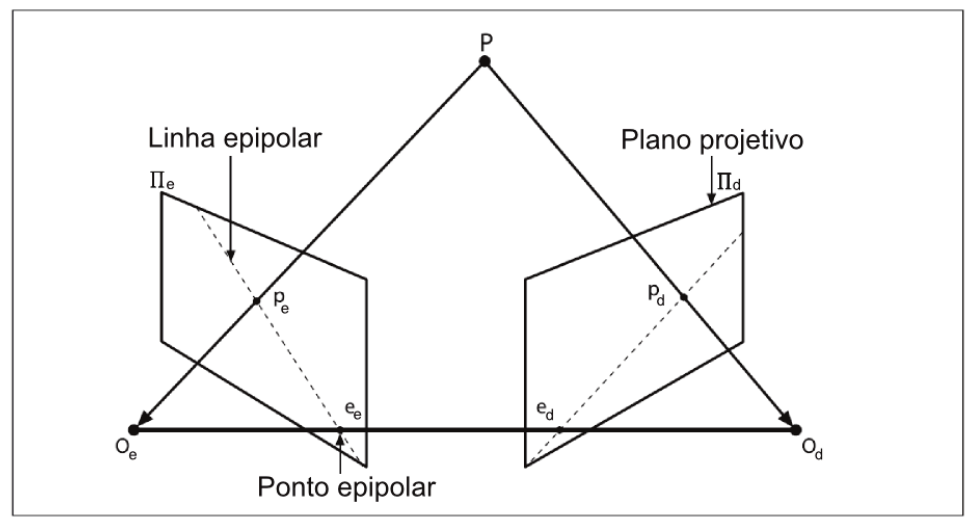
\includegraphics[scale=0.35]{./Resources/bradski/geometry_epipolar.png}
 	\caption{Geometria Epipolar. Imagem retirada de \cite{Mendes2012}}
 	\label{geometry_epipolar}
\end{figure}

Projeta-se o ponto P no centros de projeção $O^e$ e $O^d$, as linha que interligam o ponto P à esses centros interceptam os planos $\Pi_e$ e $\Pi_d$ nos pontos $p_e$ e $p_d$. Os pontos epipolares (\textit{epipoles}) $e_e$ e $e_d$ estão localizados nos pontos de intersecção da linha que interliga os centros de projeção e os planos projetivos \cite{Mendes2012}. O conhecimento desta geometria é importante pra o entendimento da chamada restrição epipolar (\textit{epipolar constraint}).

Considerando um sistema estéreo e um certo ponto $P$, deseja-se localizar na imagem da direita o seu ponto homólogo $P'$, isto é, sua projeção no plano projetivo direito. Sem a restrição, faz-se necessário a busca bidimensional em todo espaço do plano $\Pi_d$. Por outro lado, esta restrição garante que o ponto homólogo deve estar sobre a linha epipolar da imagem direita. Deste modo, é possível restringir a busca à uma única dimensão, busca somente sobre a linha epipolar, reduzindo consideravelmente o custo computacional \cite{Bradski2008}. Todavia, o sistema estéreo deve estar corretamente calibrado para que possa tomar mão desta restrição. A expressão \ref{epipolar_constraint} que representa a restrição epipolar é dada pela relação entre a matriz fundamental F e os dois pontos correspondentes, em coordenadas de pixel \cite{RobertLaganiere}.

\begin{equation}
 \label{epipolar_constraint}
 p'^TFp = 0
\end{equation}


%-----------------------------------------------------------------------------------------------------------------------------------------------------------------------------------------------
\subsection{Calibração das Câmeras - \textit{Calibration}}
\label{theory_calib}

Até o presente momento, todos os conceitos apresentados assumiam que as câmeras são idealmente alinhadas e que suas lentes não apresentavam distorção. Na realidade, os centros ópticos não são perfeitamente alinhados e a lente introduz distorções à imagem projetada no sensor da câmera. Deste modo, faz-se necessário o processo de calibração, o qual mensura estas deformidades e estima os parâmetros que consigam anular ou minimizar estas imperfeições. Isso permite que os métodos computacionais obtenham resultados mais precisos. Estes parâmetros são classificados em dois tipos específicos: intrínsecos e extrínsecos.


%----------------------------------------------------------------------------------------------------------------------------------------------------------------------------------------------
\subsubsection{Parâmetros intrínsecos}

Correspondem às propriedades intrínsecas de cada câmera, as quais são descritas pela matriz M (\textit{Intrinsic Matrix}) e o vetor D (\textit{Distortion Coefficients Vector}). A figura \ref{lenses_distortion} ilustra o modelo completo, componente radial e componente tangencial do modelo de distorções das lentes da câmera esquerda e direita, respectivamente.
\cite{OpenCVCalibrationModule}.

\begin{equation}
 M = \begin{pmatrix}
f_x & 0   & c_x\\ 
  0 & f_y & c_y\\ 
  0 & 0   & 1
\end{pmatrix}
\end{equation}

\begin{center}
  $f_x,f_y$: Distância focal
  
  $c_x,c_y$: Compensação do ponto principal
\end{center}

\begin{equation}
  D = (k_1,k_2,p_1,p_2[,k_3[,k_4,k_5,k_6]])
\end{equation}

\begin{center}
  $k_1,k_2,k_3$: Coeficientes de distorção radial simétrica
  
  $p_1,p_2$: Coeficientes de distorção tangencial (descentrada)
\end{center}

%----------------------------------------------------------------------------------------------------------------------------------------------------------------------------------------------
\subsubsection{Parâmetros extrínsecos}
Correspondem às propriedades extrínsecas, isto é, demonstram a disposição espacial da segunda câmera, direita, com relação à câmera da esquerda em coordenadas globais. Assim como ilustrado na figura \ref{essential_geometry.png}, a matriz de rotação R (3x3) e o vetor de translação T (3x1) são responsáveis por descrever este deslocamento. Geralmente, quando o quadro de referência não encontra-se no centro de projeção da câmera, faz-se necessário a adição da matriz de rotação e o vetor de translação. Neste contexto, utiliza-se o sistema de coordenadas homogêneas, isto é, pontos 2D são representados como vetores 3x1 e pontos 3D como vetores 4x1. Deste modo, tem-se que a equação \ref{projection_equation} descreve a relação do ponto $P(X,Y,Z)$ e o ponto projetado $p'$ no plano $\Pi_r$\cite{RobertLaganiere}.

%----------------------------------------------------------------------------------------------------------------------------------------------------------------------------------------------
\begin{equation}
  s.p' = M
  \begin{bmatrix}
  \begin{array}{c|c}
  R & t
  \end{array}
  \end{bmatrix}
  P 
\end{equation}

%----------------------------------------------------------------------------------------------------------------------------------------------------------------------------------------------
\begin{equation}
\label{projection_equation}
s
\begin{bmatrix}
x \\ 
y \\ 
1 
\end{bmatrix}
= 
\begin{bmatrix}
f_x & 0 & c_x\\ 
0 & f_y & c_y\\ 
0 & 0 & 1
\end{bmatrix} 
\begin{bmatrix}
r_{11} & r_{12} & r_{13} & t_1 \\ 
r_{21} & r_{22} & r_{23} & t_2 \\ 
r_{31} & r_{32} & r_{33} & t_3
\end{bmatrix}
\begin{bmatrix}
X \\ 
Y \\ 
Z \\ 
1
\end{bmatrix}
\end{equation}

%----------------------------------------------------------------------------------------------------------------------------------------------------------------------------------------------
\begin{figure}[H]
 	\centering
 	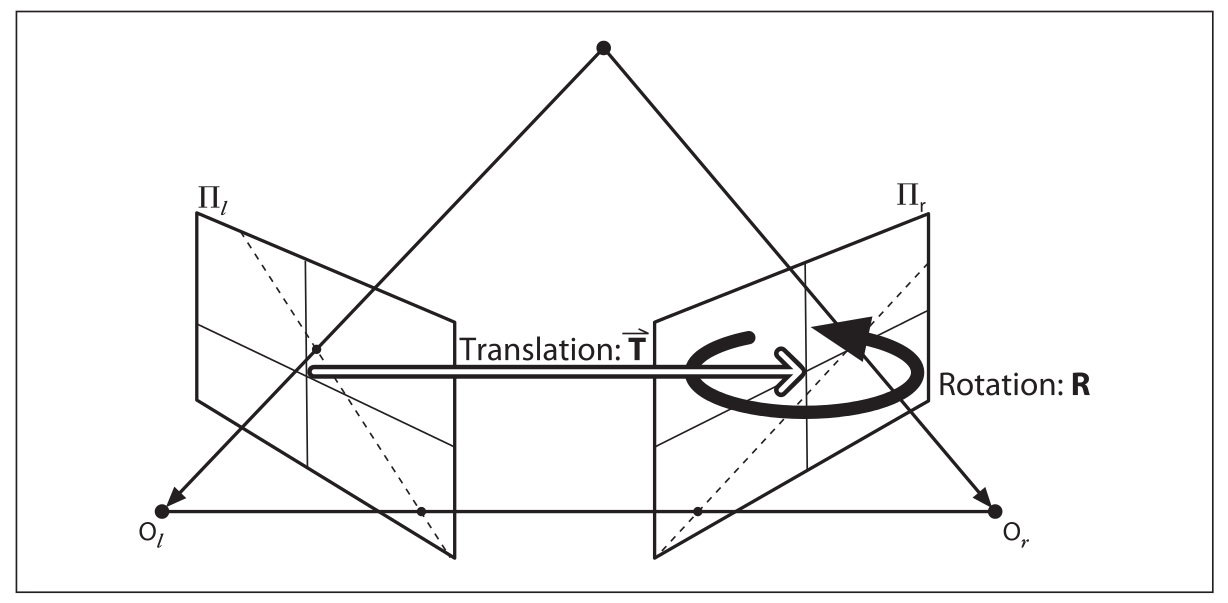
\includegraphics[scale=0.25]{./Resources/bradski/essential_geometry.png}
 	\caption{O deslocamento do plano $\Pi_r$ com relação ao plano $\Pi_l$ pode ser descrito pela matriz R e o vetor de translação T. Imagem retirada de \cite{Bradski2008}.}
 	\label{essential_geometry.png}
\end{figure}

%----------------------------------------------------------------------------------------------------------------------------------------------------------------------------------------------
Devido ao desalinhamento entre as câmeras, torna-se necessário estimar estas variáveis, aumentando, assim, a eficiência dos métodos estéreo ao procurarem pelas correspondências entre as duas imagens. A figura \ref{stereo_calib_extrinsic}, ilustra o processo de calibração dos parâmetros extrínsecos, no qual utiliza-se um conjunto de imagens do padrão de calibração. Ao fim deste processo, é possível aferir o posicionamento da segunda câmera com relação à primeira \cite{Bouguet1999}.


%----------------------------------------------------------------------------------------------------------------------------------------------------------------------------------------------
\subsection{Retificação das Imagens - \textit{Rectification}}

O processo de retificação é responsável por realizar as correções com relação à distorção das lentes e ao alinhamento das câmeras, de acordo com os parâmetros obtidos pelo processo de calibração apresentado no tópico anterior. Ao fim deste processo, deseja-se que o par de imagens estéreo esteja retificado e sem distorções, preparado para a aplicação dos métodos estéreo, assim como ilustrado na figura \ref{rectification_process}.

\begin{figure}[H]
 	\centering
 	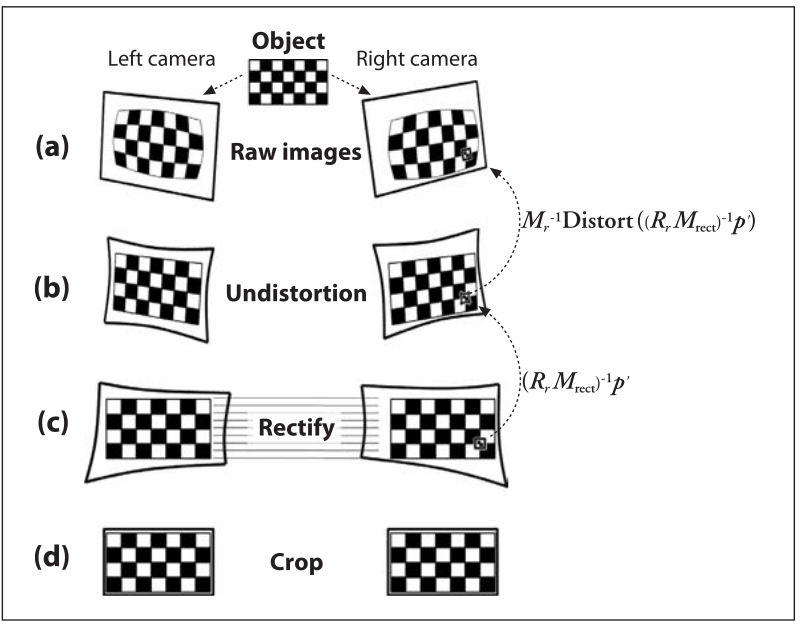
\includegraphics[scale=0.32]{./Resources/bradski/rectification_process.png}
 	\caption{Retificação de Imagens - Processo de retificação estéreo. Imagem retirada de \cite{Bradski2008}.}
 	\label{rectification_process}
\end{figure}


%-----------------------------------------------------------------------------------------------------------------------------------------------------------------------------------------------
\subsection{Correspondência Estéreo - \textit{Stereo Correspondence}}

Correspondência estéreo não é nada mais que a utilização de métodos estéreo, os quais são responsáveis pela procura de pontos homólogos nos pares de imagens estéreo. Como visto anteriormente, devido ao distanciamento das câmeras $(T)$ e ao distanciamento do objeto com relação às câmeras $(Z)$, o mesmo ponto apresenta diferentes posicionamento nos planos das câmeras $x^l$ e $x^r$. A figura \ref{homologous_points _stereo} ilustra um par de imagens estéreo (esquerda e direita) e o mapa de disparidades gerado pela cena, nas quais os pixels homólogos estão destacados. Os métodos estéreo utilizam da restrição epipolar o que reduz o espaço de busca e de diferentes meios para encontrá-los. Mesmo com essa essa restrição e com a retificação das imagens, os métodos ainda assim apresentam um elevado custo computacional, além do que ainda estão sujeitos à encontrarem falsas correspondências. 

\begin{figure}[H]
 	\centering
 	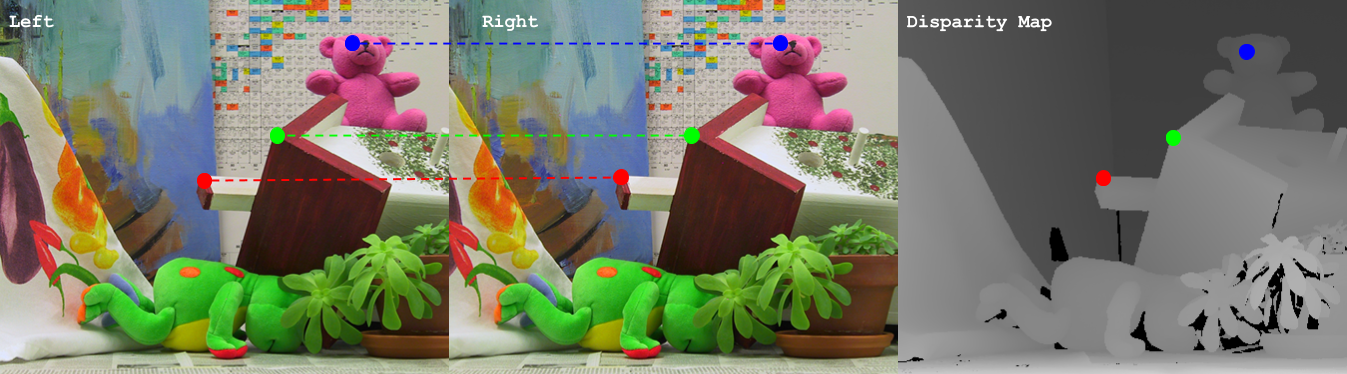
\includegraphics[scale=0.33]{./Resources/homologous_points_stereo.png}
 	\caption{Correspondência de pontos homólogos em um par de imagens estéreo. Imagem original retirada de \cite{Scharstein2003}.}
 	\label{homologous_points _stereo}
\end{figure}


%-----------------------------------------------------------------------------------------------------------------------------------------------------------------------------------------------
\subsubsection{Mapa de disparidades - \textit{Disparity Map}}

Como já foi dito anteriormente, disparidade é o deslocamento dos pontos homólogos entre as duas imagens. Nos métodos estéreo, o valor da disparidade é codificada em escala de cinza, a qual é inversamente proporcional à distância do objeto, assim como representado na figura \ref{depth_disparity}. Assim, níveis de cinza mais altos (tons claros) correspondem a disparidades maiores (perto) e níveis de cinza mais baixos (tons escuros) correspondem a disparidades mais baixas (distante). Devido a sua relação com a distância, este conceito é comumente atrelado à percepção de profundidade.

\begin{figure}[H]
 	\centering
 	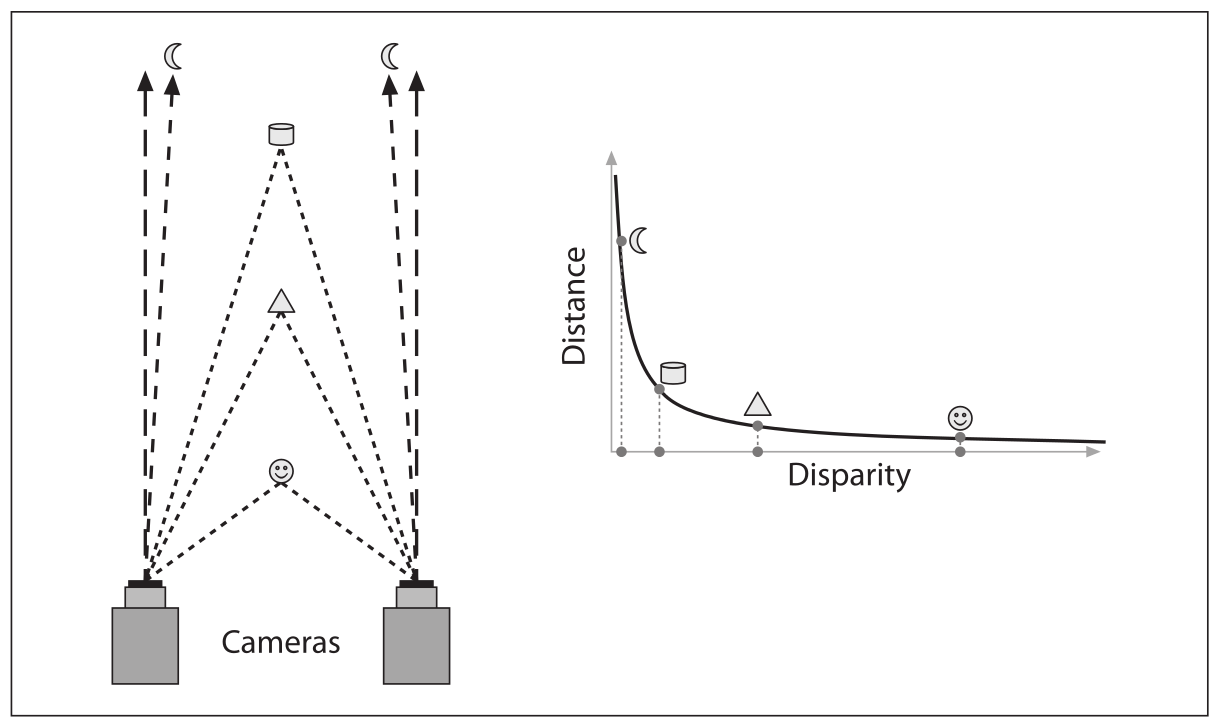
\includegraphics[scale=0.3]{./Resources/bradski/depth_disparity.png}
 	\caption{Relação inversamente proporcional entre distância e disparidade. Imagem retirada de \cite{Bradski2008}}
 	\label{depth_disparity}
\end{figure}

%-----------------------------------------------------------------------------------------------------------------------------------------------------------------------------------------------
\subsubsection{Métodos Estéreo}

A seguir, encontra-se apresentado um pequeno resumo de como são os operadores dos métodos estéreo utilizado neste trabalho.

\begin{enumerate}
 \item \textbf{\textit{Block Matching} - BM:} Este algoritmo é um método local, no qual utiliza soma das diferenças ao quadrado (SSD - \textit{Sum of Squared Differences}) para a determinação de correspondências. O tamanho da vizinhança deve ser avaliado, visto que a densidade do mapa gerado, nível de detalhamento e intensidade de ruído dependem disso. Caso o bloco seja pequeno, o mapa apresentará detalhes mais nítidos, porém adicionará ruídos ao mapa. Por outro lado, um bloco maior reduz o nível de ruído, porém diminui o nível de detalhamento do mapa. As limitações serviram de motivação para a criação do método a seguir \cite{Hirschmuller2008}.   
 \item \textbf{\textit{Semi-global Block Matching} - SGBM:} Este algoritmo é um método global e também visa a obtenção de uma correspondência estéreo mais precisa, para isso, além da etapa de agregação de custo (cálculo da similaridade), modela-se o sistema como um problema de minimização energética \cite{JunhwanKim2003}. Por conta disso, este método é mais lento que o apresentado anteriormente, porém é mais denso ao comparar-se o nível de detalhamento para um bloco de tamanho pequeno \cite{Hirschmuller2008}.
 \item \textbf{\textit{Block Matching with GPU Acceleration} - BMGPU:} Método é igual ao primeiro apresentado, diferindo do fato que as suas bibliotecas e métodos implementados são voltados para a aceleração em GPU (\textit{Graphics Processing Unit}). Dado o paralelismo inerente dos aceleradores gráficos de hoje, esse tipo de \textit{hardware} permite o processamento simultâneo dos dados. 
\end{enumerate}


% TODO: Escrever sobre os dois tipos de pesquisa que existem atualmente: Fast Stereo vs. High-Confidence Stereo
%Atualmente,

% TODO: Escrever os melhores metódos estéreo que existem hoje: http://www.cvlibs.net/datasets/kitti/eval_stereo_flow.php?benchmark=stereo.

% TODO: Escrever seção de Projeção Tridimensional(Opcional)
%-----------------------------------------------------------------------------------------------------------------------------------------------------------------------------------------------
%\section{Projeção Tridimensional - \textit{3D Reprojection}}


% TODO: Escrever seção de Reconhecimento de Objetos(Opcional)
%-----------------------------------------------------------------------------------------------------------------------------------------------------------------------------------------------
%\section{Reconhecimento de Objeto - \textit{Object Recognition}}
%\subsection{Segmentação - \textit{Image Segmentation}}

%\subsection{Identificação - \textit{Object Identification}}


%-----------------------------------------------------------------------------------------------------------------------------------------------------------------------------------------------
\subsection{Aplicações em Robótica}
\label{aplicacoes_robotica}
Nesta seção, serão apresentados alguns dos trabalhos que têm como principais sensores câmeras estéreo para a navegação autônoma em ambientes terrestre, aérea e subaquática.

Nos dias de hoje, as empresas automobilísticas vem participando de uma verdadeira corrida tecnológica para o desenvolvimento de automóveis totalmente autônomos e economicamente viáveis. As universidades não ficaram para trás e também apresentam pesquisas envolvendo desenvolvimento de algoritmos de controle e sensores, tornando essa corrida ainda mais acirrada. Os resultados apresentados são realmente promissores, e concretizam cada vez mais essa realidade tida até então como distante. Na figura \ref{caminhao_autonomo}, é possível observar o projeto de caminhão autônomo desenvolvido pelo Laboratório de Robótica Móvel - LRM - ICMC/USP. O caminhão conta com diversos sensores, dentre eles câmeras estéreo, que identificam outros automóveis, pessoas e faixas de sinalização \cite{ShinzatoP}. 

%-----------------------------------------------------------------------------------------------------------------------------------------------------------------------------------------------
\begin{figure}[H]
 	\centering
 	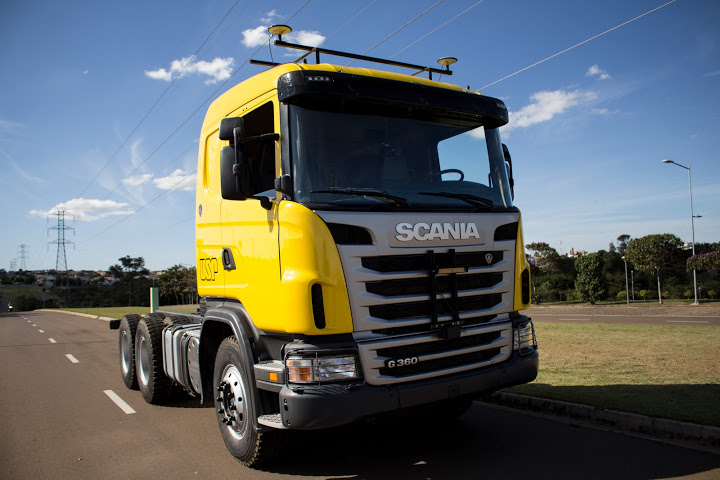
\includegraphics[scale=0.40]{./Resources/caminhao_autonomo.jpg}
 	\caption{Caminhão Autônomo desenvolvido pelo Laboratório de Robótica Móvel - LRM - ICMC/USP em parceria com a Scania.}
 	\label{caminhao_autonomo}
\end{figure}

%-----------------------------------------------------------------------------------------------------------------------------------------------------------------------------------------------
No caso de navegação autônoma para ambiente aéreo, o projeto utilizando \textit{Micro Air Vehicle} (MAVS) desenvolvido pelo \textit{Massachusetts Institute of Technology} (MIT) permite que pequenas aeronaves consigam navegar autonomamente e desviar de obstáculos voando a um velocidade de 30 mph (48 $km/h$). A figura \ref{mit_drones} apresenta o trabalho desenvolvido, o qual é um comparativo de desempenho de uma implementação em hardware utilizando \textit{Field-programmable gate array} (FPGA) e um processador ARM para processamento embarcado do método SGBM \cite{BarryMIT}.

%-----------------------------------------------------------------------------------------------------------------------------------------------------------------------------------------------
\begin{figure}[H]
 	\centering
 	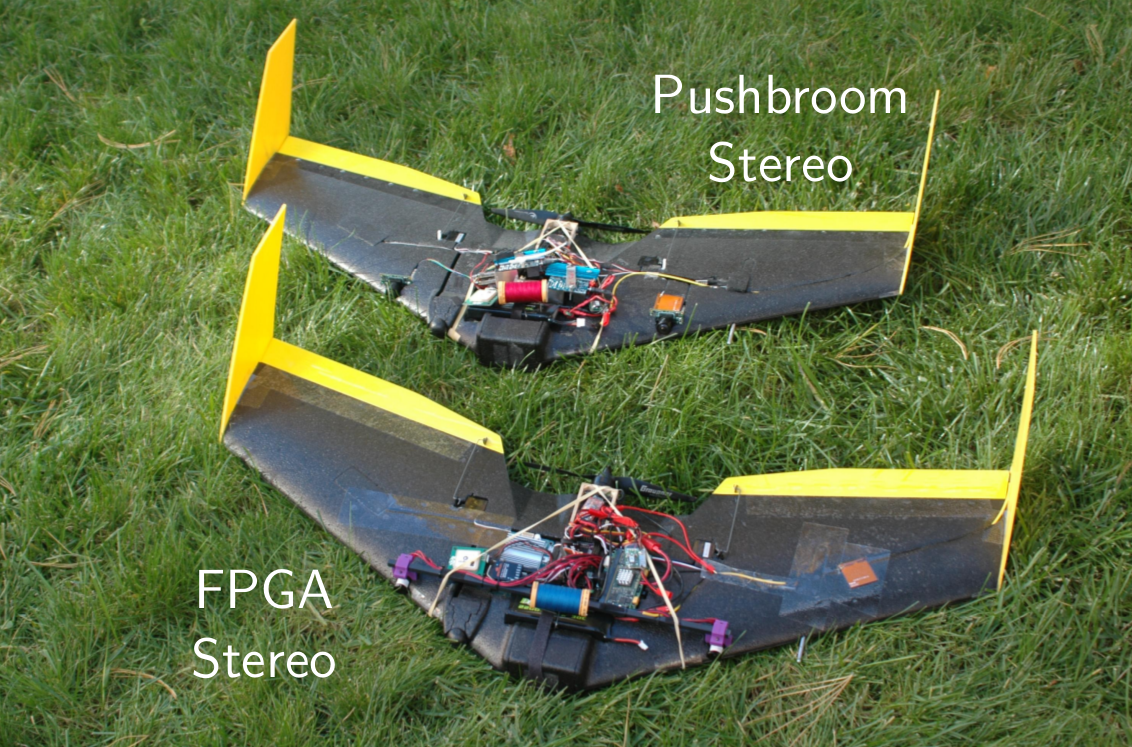
\includegraphics[scale=0.26]{./Resources/mit_drones.png}
 	\caption{Plataformas experimentais de aeronaves com o Sistema Estéreo - FPGA e o Sistema Estéreo - Pushbroom. Câmaras são montados na parte dianteira das asas na mesma linha de base (34 cm) em ambas células. Imagem retirada de \cite{BarryMIT}.}
 	\label{mit_drones}
\end{figure}

%-----------------------------------------------------------------------------------------------------------------------------------------------------------------------------------------------
No caso de navegação autônoma para ambiente subaquático, um exemplo de \textit{autonomous underwater vehicle} (AUV) é o projeto desenvolvido pela Universidade espanhola de Girona (veja figura \ref{G500}). O trabalho propõe a utilização do método de Mapeamento e Localização Simultânea (SLAM), juntamente com câmera estéreo, para o reconhecimento do ambiente, aprimorando assim o erro de rastreamento dos objetos \cite{Nagappa2013}.

%-----------------------------------------------------------------------------------------------------------------------------------------------------------------------------------------------
\begin{figure}[H]
 	\centering
 	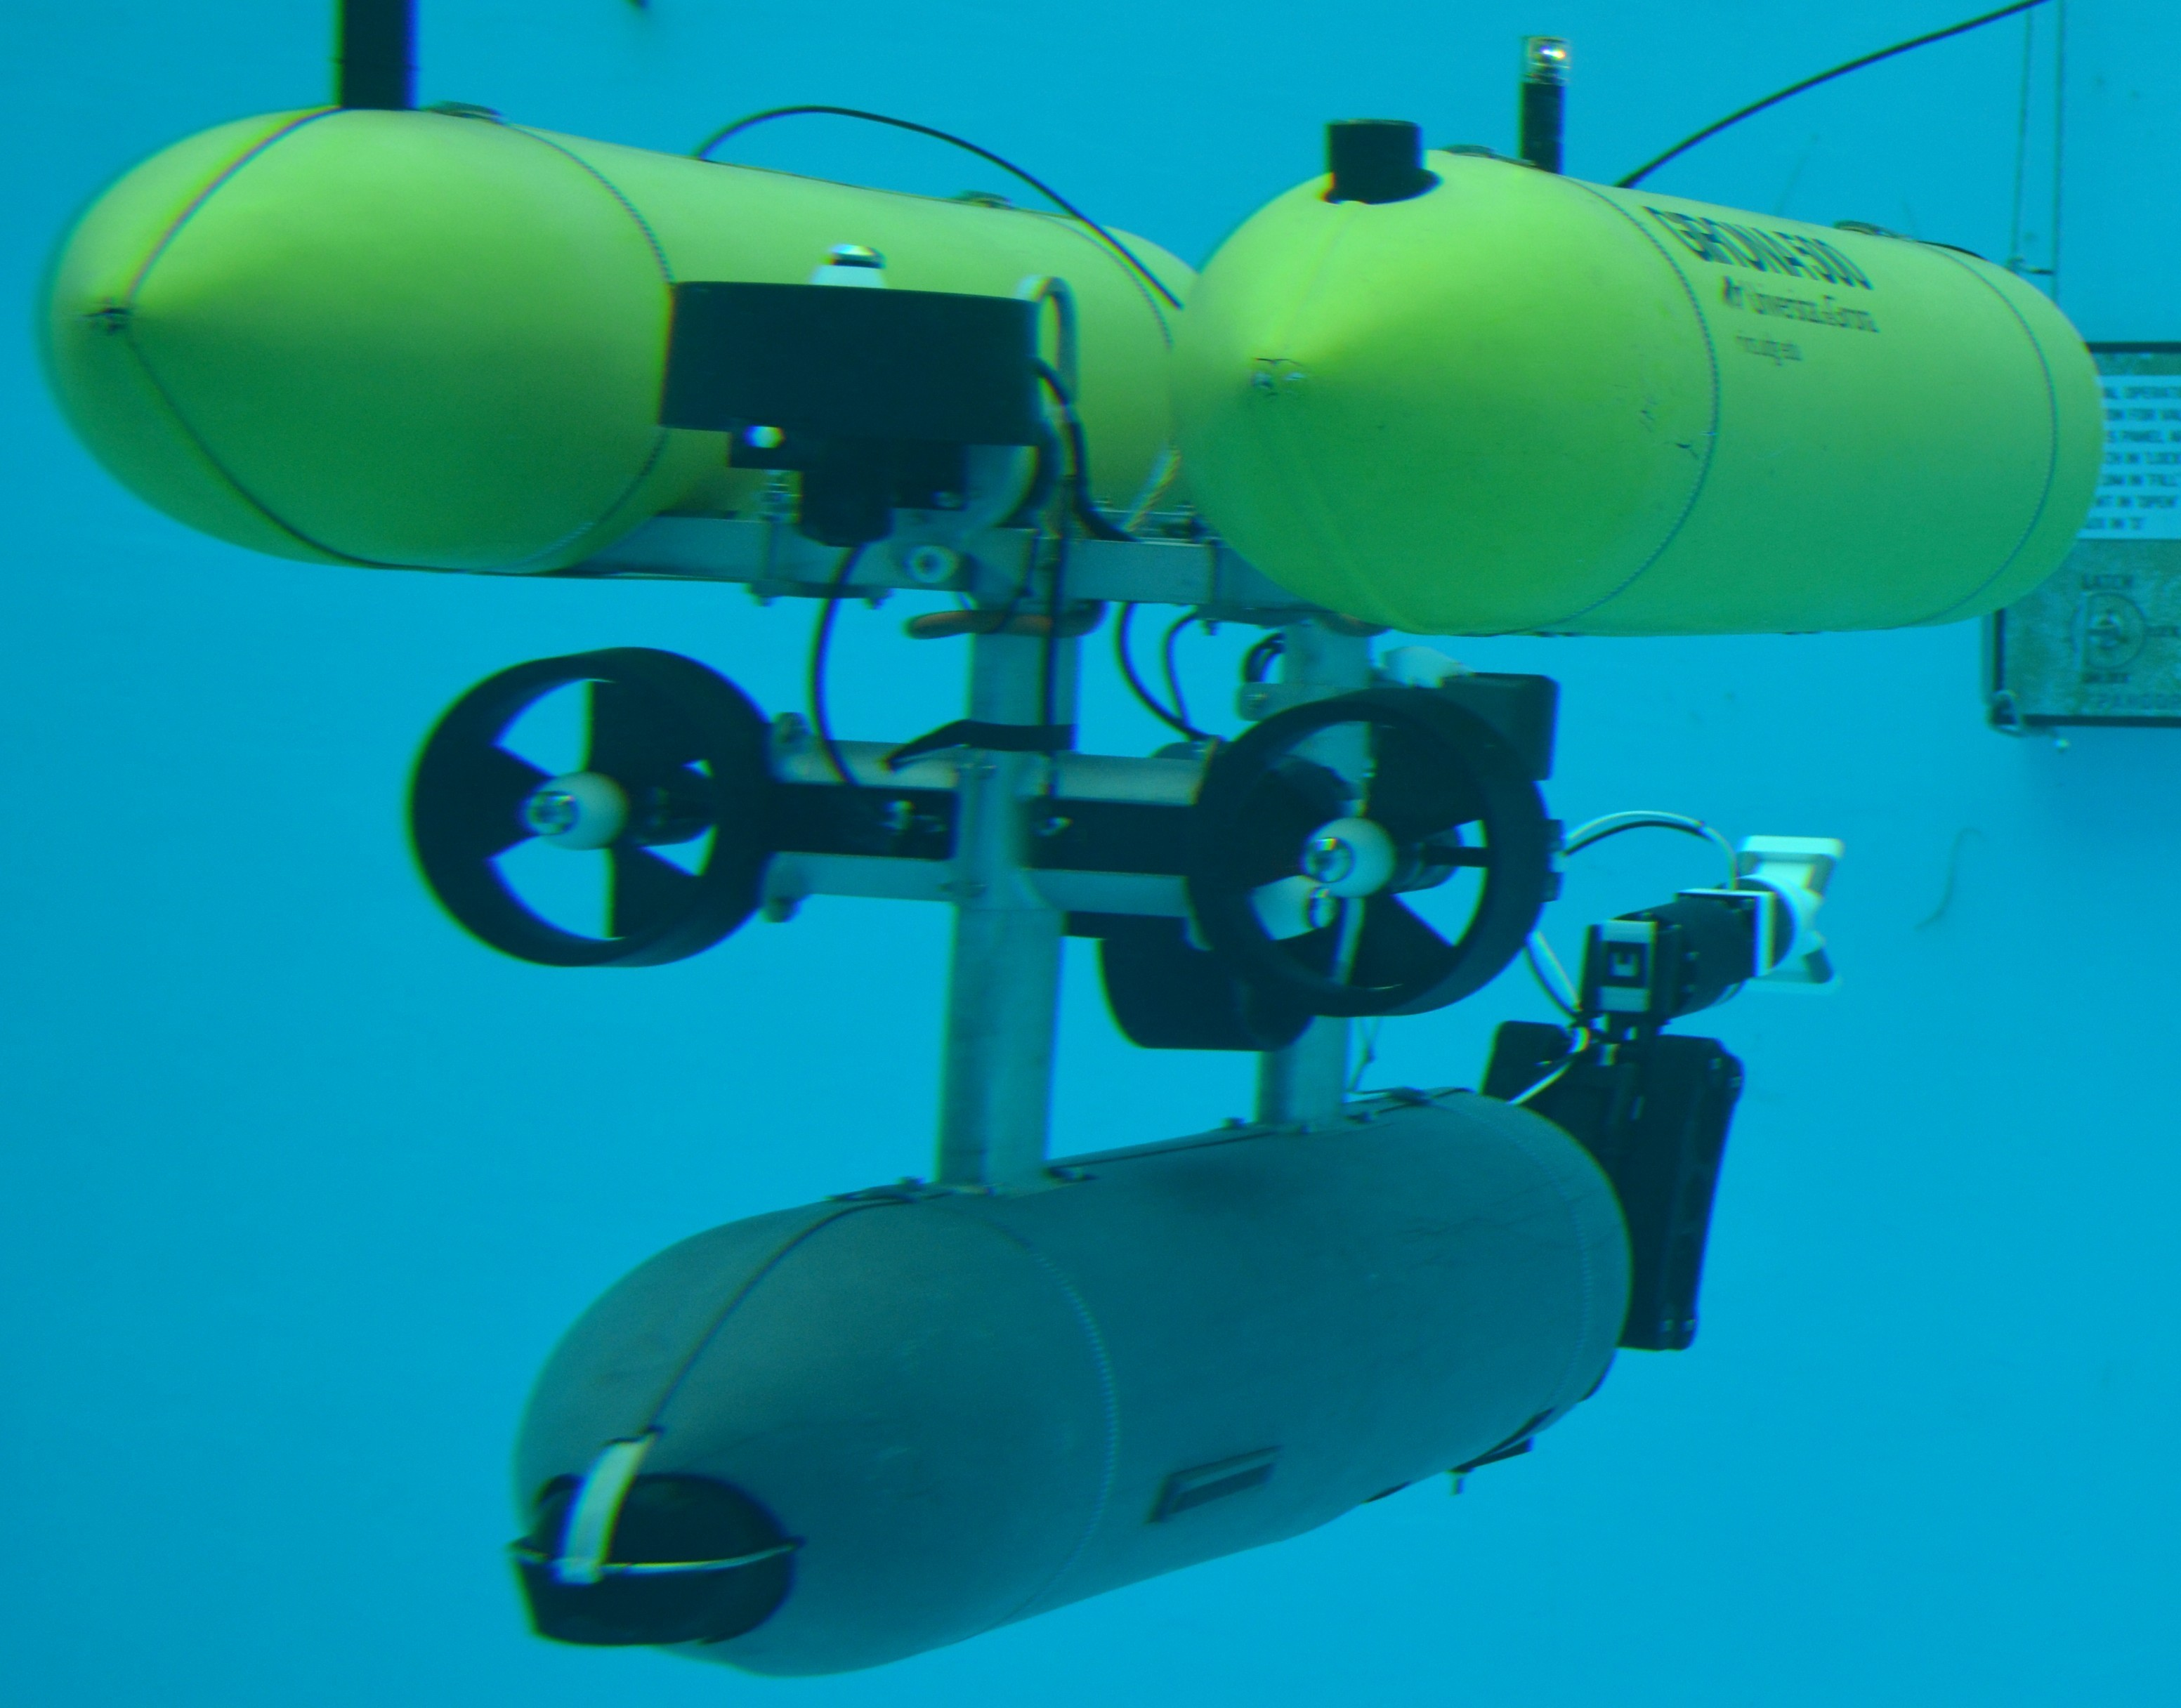
\includegraphics[scale=0.1]{./Resources/G500.jpg}
 	\caption{Veículo Submarino Autônomo - Girona 500}
 	\label{G500}
\end{figure}

%-----------------------------------------------------------------------------------------------------------------------------------------------------------------------------------------------
\section{OpenCV}
\textit{Open Source Computer Vision Library} (OpenCV) é uma biblioteca de código aberto, a qual reúne diversos algoritmos relacionados a visão computacional. O OpenCV foi criado pelo centro de pesquisa da \textit{Intel}, e atualmente é mantido pelo time de pesquisadores da companhia \textit{Itseez} \cite{ItseezOpenCVinfo}. A biblioteca é estruturada em diferentes módulos, os quais agrupam os algoritmos relacionados a tópicos como processamento de imagem, estimativa de movimento, correspondência estéreo, extratores de características, criação de interfaces de usuário e aceleração em \textit{hardware}. O OpenCV foi criado com a intensão de ser multiplataforma, por conta disso, em sua maior parte, foi escrito em linguagem C/C++, o que o torna facilmente portável para diversas plataformas como Windows, Linux, Android, MacOS, iOS, dentre outros. Recentemente, módulos dando suporte à CUDA (seção \ref{cuda}) e OpenGL foram incorporados à biblioteca expandindo ainda mais o número de aplicações possíveis \cite{ItseezOpenCVPlatforms}. 


%-----------------------------------------------------------------------------------------------------------------------------------------------------------------------------------------------
\section{Linux Embarcado}

Linux é um sistema operacional de código-aberto que é amplamente utilizado, cujo \textit{Kernel}, originalmente escrito por Linus Torvalds, pode suportar diversos designs de sistemas podendo ser um computador pessoal, um supercomputador ou \textit{cluster}, ou até mesmo sistemas \textit{System-on-Chip} (SoC). Este sistema é capaz de suportar diversas arquiteturas de processadores como x86{\_}64, PowerPC, ARM, MIPS, StrongARM, XScale, dentre outras \cite{Wang2011}.

O popularização do termo Linux fez com que atualmente exista uma certa confusão sobre a distinção de um \textit{Kernel} de um sistema operacional e do sistema operacional propriamente dito. A maior razão desta confusão é a variedade de distribuições desenvolvidas pela comunidade, visto a facilidade para customizar seus módulos, pacotes, sistemas de arquivo e servidores gráficos. Dada sua versatilidade, logo tornou-se a peça chave para o desenvolvimento de sistemas embarcados, os quais são computadores completamente especializados para a realização de tarefas específicas. Esses sistemas diferem de computadores de propósito geral e comumente apresentam certa restrições de dimensão, condições de operação, ou limitação de recursos computacionais como menor poder de processamento ou menor capacidade de armazenamento. 

Assim, começaram a surgir distribuições de Linux, os chamados \textit{Embedded Linux}, que apresentavam menores requisitos de sistemas, devido à remoção de módulos que não são utilizados em determinados sistemas ou à otimização desses módulos para aquela atividade específica \cite{Yaghmour2008}.


%-----------------------------------------------------------------------------------------------------------------------------------------------------------------------------------------------
\section{Aceleração em Hardware - CUDA}
\label{cuda}

\textit{Compute Unified Device Architecture} (CUDA) é uma tecnologia desenvolvida pela NVIDIA e em sua essência é uma plataforma de computação paralela de propósito geral, cujo objetivo é tirar proveito das unidades de processamento gráfico (GPU), assim, acelerando consideravelmente a execução de algoritmos computacionais complexos ao comparar-se com o desempenho da CPU.

Atualmente, a maioria das placas de video da NVIDIA contam com essa tecnologia, por conta disso os pesquisadores e desenvolvedores de software estão voltando suas pesquisas para o desenvolvimento e otimização de algoritmos que possam explorar todo o poder de processamento destes dispositivos. Alguns exemplos de aplicações são identificação de placas ocultas em artérias, análise do fluxo de tráfego aéreo \cite{Monish2011} e visualização de moléculas \cite{Stone2015}.

Historicamente, a implementação de algoritmos em GPU mostrou-se bastante obscura, visto que sua programação era bastante atrelada ao hardware a ser utilizado, mesmo com linguagens de programação gráfica como o OpenGL. Em 2003, um grupo de pesquisadores de Stanford, apresentou o primeiro compilador, Brook, que facilitaria a implementação de software, visto que permitia lidar de uma maneira mais maleável o fluxo de dados, podendo principalmente paralelizá-los. Em 2006, a NVIDIA juntamente com Ian Buck, criador do Brook, desenvolveram uma plataforma (CUDA) mais intuitiva e que permitisse a utilização de uma linguagem de alto nível e tornasse a GPU em um processador de propósito geral (GPGPU) \cite{NVIDIA}.

\chapter{Materiais e Métodos}
\label{Materiais}

%\textcolor{red}{\textbf{Dica:} Materiais e Métodos: descrição clara dos procedimentos e dos materiais
%adotados para o desenvolvimento do trabalho (sem resultados) ? incluindo sua
%adequação ao trabalho.
%Tem que responder às perguntas:
%-está com um tamanho adequado (proporcional) à monografia?
%-há informação suficiente e clara sobre os materiais e sobre os métodos
%adotados?
%Não há necessidade de reproduzir (copiar) as obras que embasam o trabalho e
%sim colocar o suficiente para o entendimento do trabalho e citar as referências.}

Nesta seção serão apresentados os equipamentos necessários e métodos utilizados para o desenvolvimento do projeto. No caso dos equipamentos, serão apresentados todas as especificações técnicas e sua importância para o trabalho. Na seção destinada aos métodos, os algoritmos desenvolvidos para identificação e reconhecimento de objetos serão descritos.

%------------------------------------ Materiais -----------------------------------------------------
\section{Materiais}
Com relação aos equipamentos é possível classificá-los em três grupos distintos:
Câmeras estereoscópicas, Unidades de Processamento, e Equipamentos auxiliares.

\subsection{Câmeras estereoscópicas}

O projeto já utilizou duas câmeras estereoscópicas. Primeiramente, utilizou-se a \textit{webcam} Minoru(veja figura \ref{minoru}), visto que apresentava preço totalmente acessível e cumpria o requisito de realizar \textit{streaming} via USB. Deste modo, tornou-se um equipamento essencial para a implementação dos métodos para encontro de correspondências entre as câmeras. A tabela \ref{minoru_tab}	 apresenta as especificações da \textit{webcam}.

\begin{figure}[H]
 	\centering
 	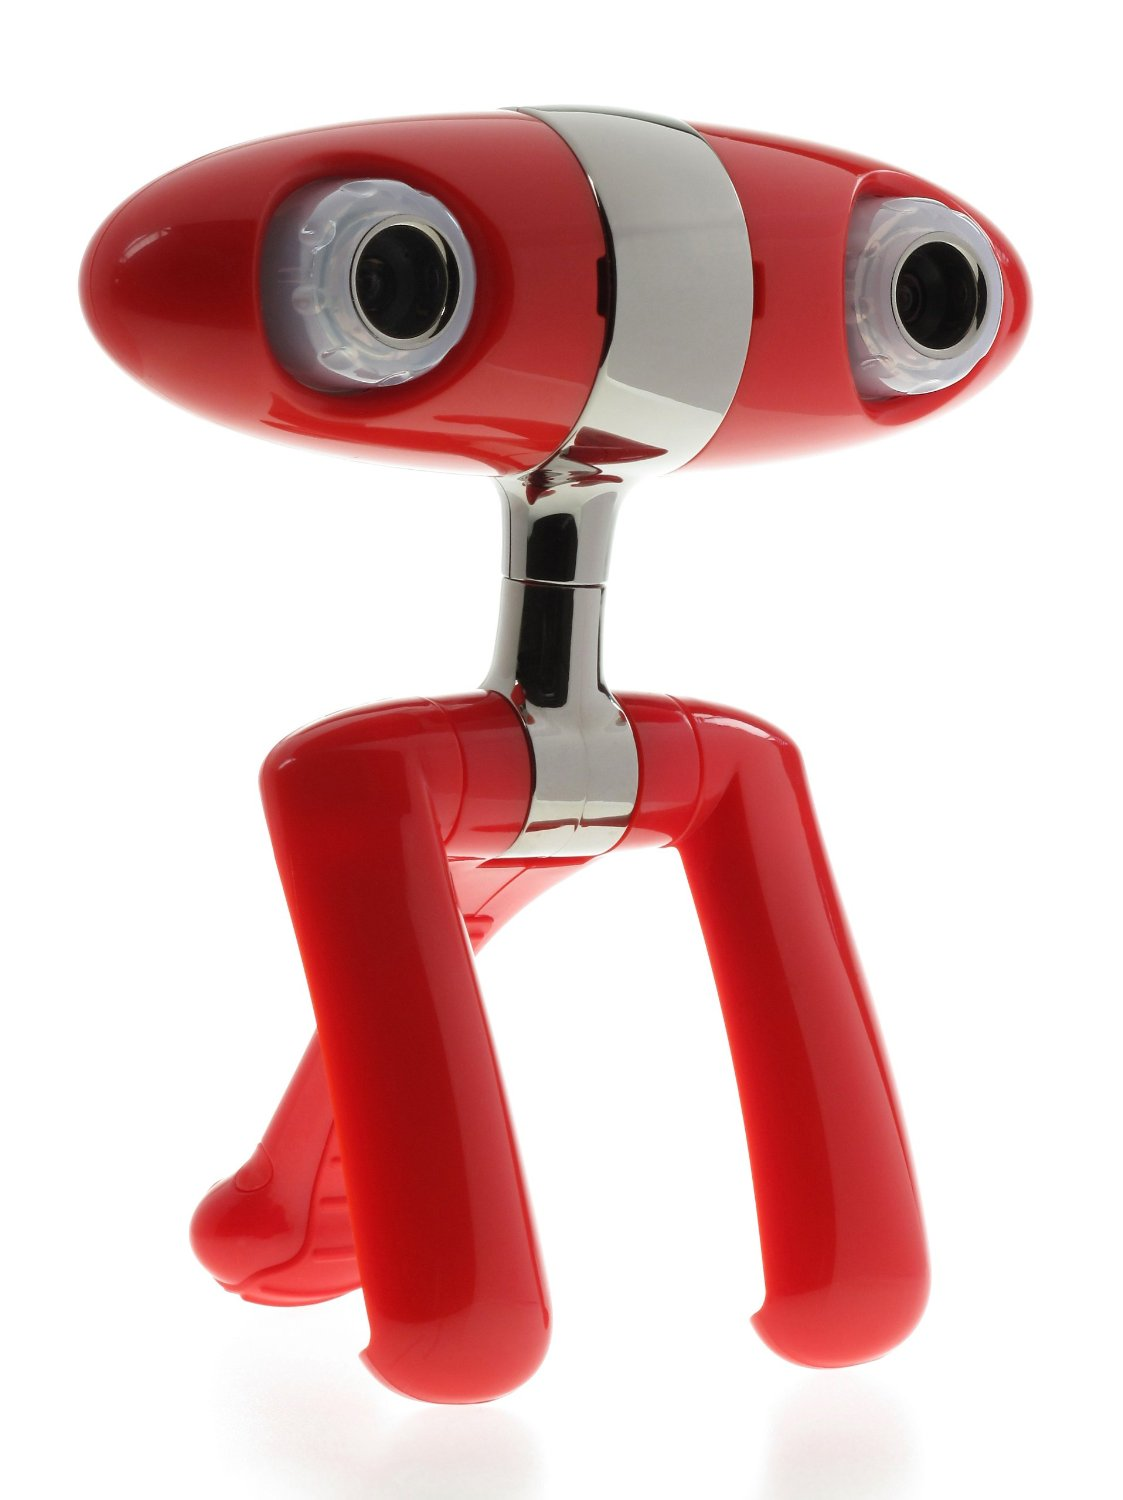
\includegraphics[scale=0.10]{./Resources/minoru.jpg}
 	\caption{3D Webcam Minoru}
 	\label{minoru}
\end{figure}

\begin{table}[]
\centering
\caption{Especificações - 3D Webcam Minoru}
\label{minoru_tab}
\begin{tabular}{ll}
\textbf{Sensor de Imagem}      & VGA CMOS Sensor  	\\
\textbf{Resolução Máxima}      & $800x600$        	\\
\textbf{Tamanho Linha de Base} & 6 cm             	\\
\textbf{Taxa de Captura}       & 30 fps             	\\
\textbf{Distância Focal}       & 10 cm até $\infty$	\\
\textbf{Campo de Visão}        & $42\degree$		   	\\
\textbf{Peso}				  & 249.48 g				\\
\end{tabular}
\end{table}

Atualmente, a câmera utilizada é uma câmera digital 3D W3 fabricada pela Fujifilm (veja figura \ref{fujiW3}). A primeira câmera foi substituída, pois o controlador USB não permitia que a webcam realizasse \textit{streaming} na máxima resolução. Deste modo, optou-se por uma câmera com maior resolução e que apresentasse lentes com baixa distorção. Entretanto, essa câmera não apresenta \textit{streaming} via USB, assim é necessário que os vídeos sejam processados \textit{offline}. Visto que o projeto preocupa-se principalmente na identificação de obstáculos, isso não oferece nenhuma desvantagem para o desenvolvimento do algoritmo. Todavia, para uma aplicação real, a câmera instalada no veículo deve apresentar esse aspecto. A tabela \ref{fujiW3_tab} apresenta as especificações da câmera.

\begin{table}[]
\centering
\caption{Especificações - Câmera Digital Fujifilm FinePix Real 3D W3}
\label{fujiW3_tab}
\begin{tabular}{ll}
\textbf{Sensor de Imagem}      & 10 MP CCD Sensor  	\\
\textbf{Resolução Máxima}      & $1280x720$        	\\
\textbf{Tamanho Linha de Base} & 7.5 cm             	\\
\textbf{Taxa de Captura}      & 24 - 30 fps          \\
\textbf{Distância Focal}       & 60 cm até $\infty$	\\
\textbf{Peso}       		      & 250g					\\
\end{tabular}
\end{table}

\begin{figure}[H]
 	\centering
 	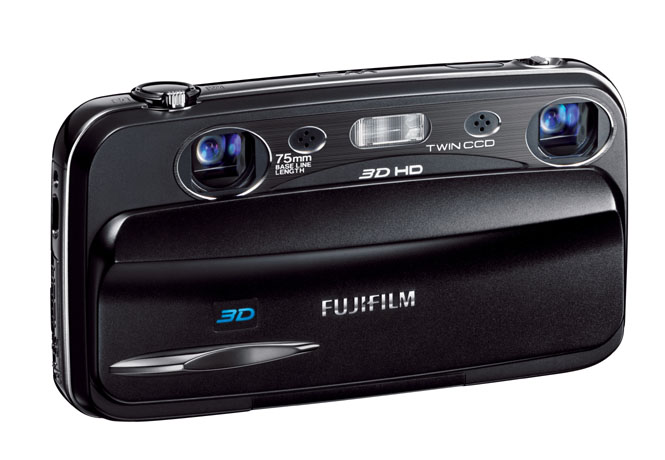
\includegraphics[scale=0.35]{./Resources/fujiW3.jpg}
 	\caption{Câmera Digital Fujifilm FinePix Real 3D W3}
 	\label{fujiW3}
\end{figure}

\subsection{Unidades de Processamento}

Visto que este trabalho também busca a implementação dos algoritmos de detecção de obstáculos em quadricópteros, tem-se como objetivo sua implementação para Linux embarcado. Abaixo estão apresentadas as plataformas que serão utilizadas para este propósito.

A primeira plataforma a ser utilizada e estudada é a plataforma aberta BeagleBone Black, ilustrada na figura \ref{bbb}. Esta plataforma foi escolhida devido ao seu tamanho reduzido, podendo ser facilmente embarcado, e ao seu poder de processamento, utiliza Cortex-A8 operando à 1 GHz. A tabela \ref{bbb_tab} apresenta as especificações da plataforma.

\begin{table}[]
\centering
\caption{Especificações - BeagleBone Black}
\label{bbb_tab}
\begin{tabular}{ll}
\textbf{Processador}           & 1GHz TI Sitara AM3359 ARM Cortex-A8					 \\
\textbf{RAM}                   & 512 MB DDR3L @ 400 MHz								 \\
\textbf{Armanezamento}         & 2 GB on-board eMMC, MicroSD                   		 \\
\textbf{Sistemas Operacionais} & Angstrom (Default), Ubuntu, Android, dentre outros...	 \\
\textbf{Consumo de energia}    & 210-460 mA @ 5V                                      	 \\
\textbf{Pinos de GPIO}         & 65/92 pinos                                            \\
\textbf{Periféricos}           & 1 USB Host, 1 Mini-USB Client, 1 10/100 Mbps Ethernet                                 
\end{tabular}
\end{table}

\begin{figure}[H]
 	\centering
 	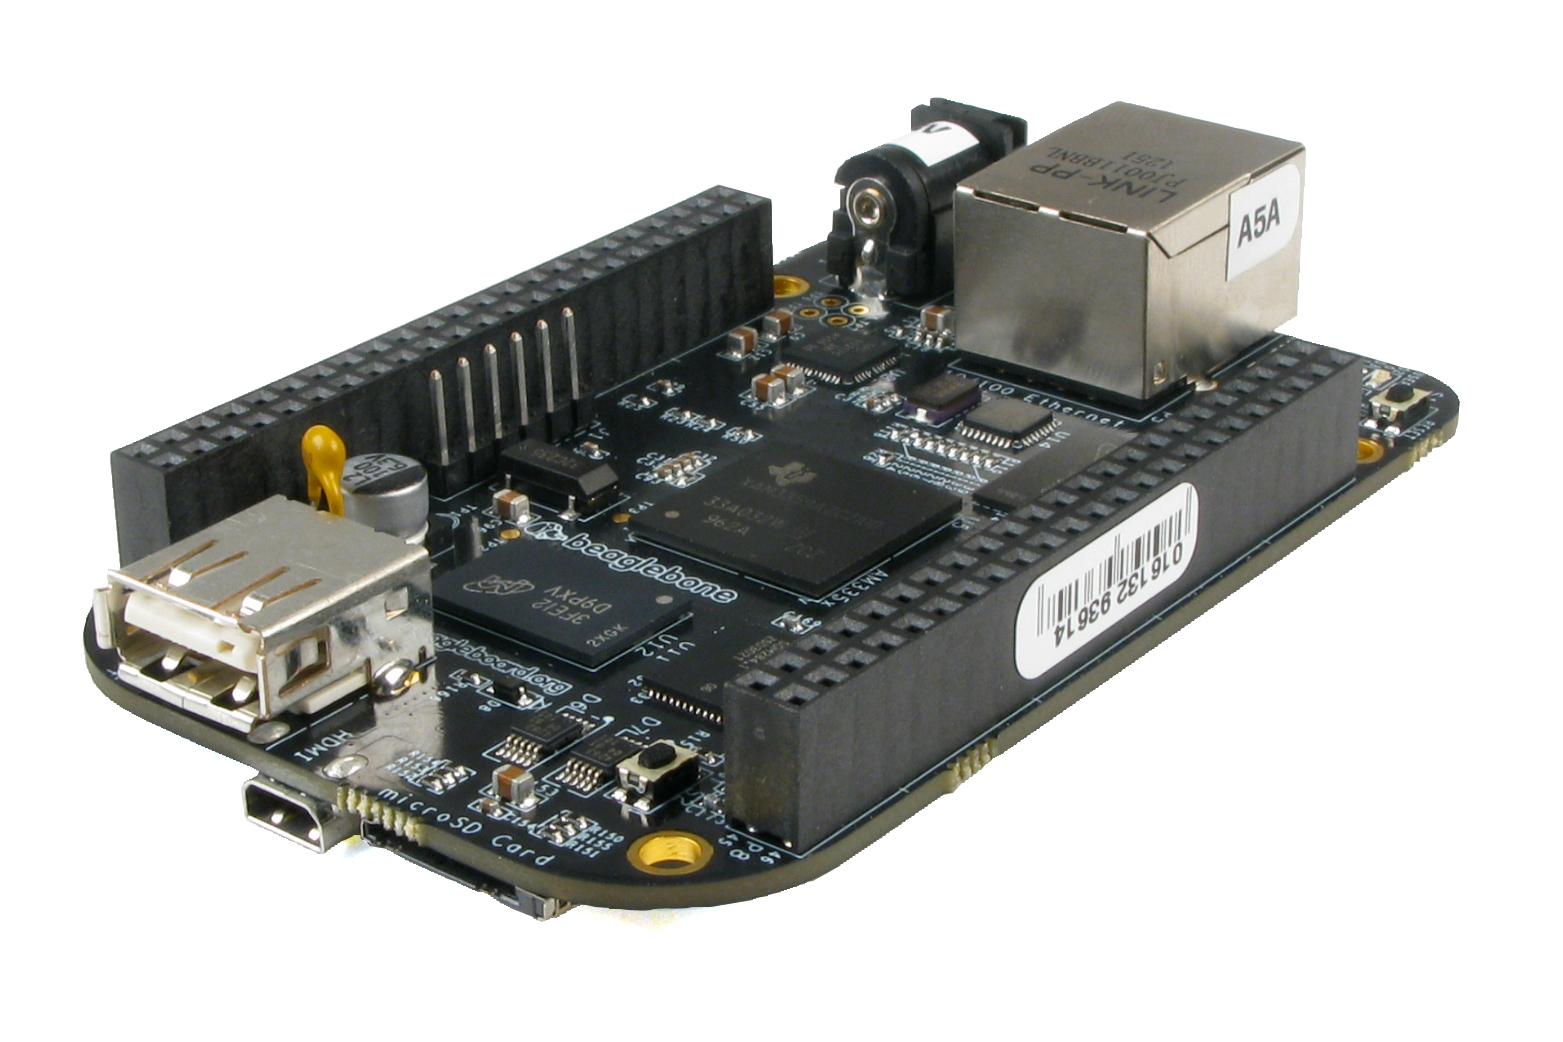
\includegraphics[scale=0.10]{./Resources/bbb.jpg}
 	\caption{Plataforma de Desenvolvimento - BeagleBone Black}
 	\label{bbb}
\end{figure}

A segunda plataforma a ser utilizada e estudada é a plataforma Jetson TK1 produzida pela NVIDIA, figura \ref{jetson_tk1}. Essa plataforma conta com um processador de 32-bits Tegra K1 baseado na tecnologia ARM Cortex-A15. O motivo pelo qual esta plataforma foi escolhida é devido ao seu poder de processamento gráfico, visto que apresenta 192 núcleos gráficos, sendo assim adequada para aplicações envolvendo processamento de imagens. A tabela \ref{jetson_tk1_tab} apresenta as especificações da plataforma.

\begin{table}[]
\centering
\caption{Especificações - Jetson TK1}
\label{jetson_tk1_tab}
\begin{tabular}{ll}
\textbf{Processador}           & NVIDIA 2.32GHz ARM quad-core Cortex-A15              \\
\textbf{Processador Gráfico}   & NVIDIA Kepler "GK20a" GPU  with 192 SM3.2 CUDA cores \\
\textbf{DRAM}                  & 2GB DDR3L 933MHz EMC x16 using 64-bit data width     \\
\textbf{Armanezamento}         & 16GB fast eMMC 4.51 (routed to SDMMC4)               \\
\textbf{Sistemas Operacionais} & Platforma 64-bit Linux Ubuntu 14.04                  \\
\textbf{Consumo de energia}    & 0.6W to 3W @ 12 V                                    \\
\textbf{Pinos de GPIO}         & 7 x GPIO pins (1.8V)                                 \\
\textbf{Periféricos}           & USB, mini-PCIe, SATA, SD-card, HDMI, audio          
\end{tabular}
\end{table}

\begin{figure}[H]
 	\centering
 	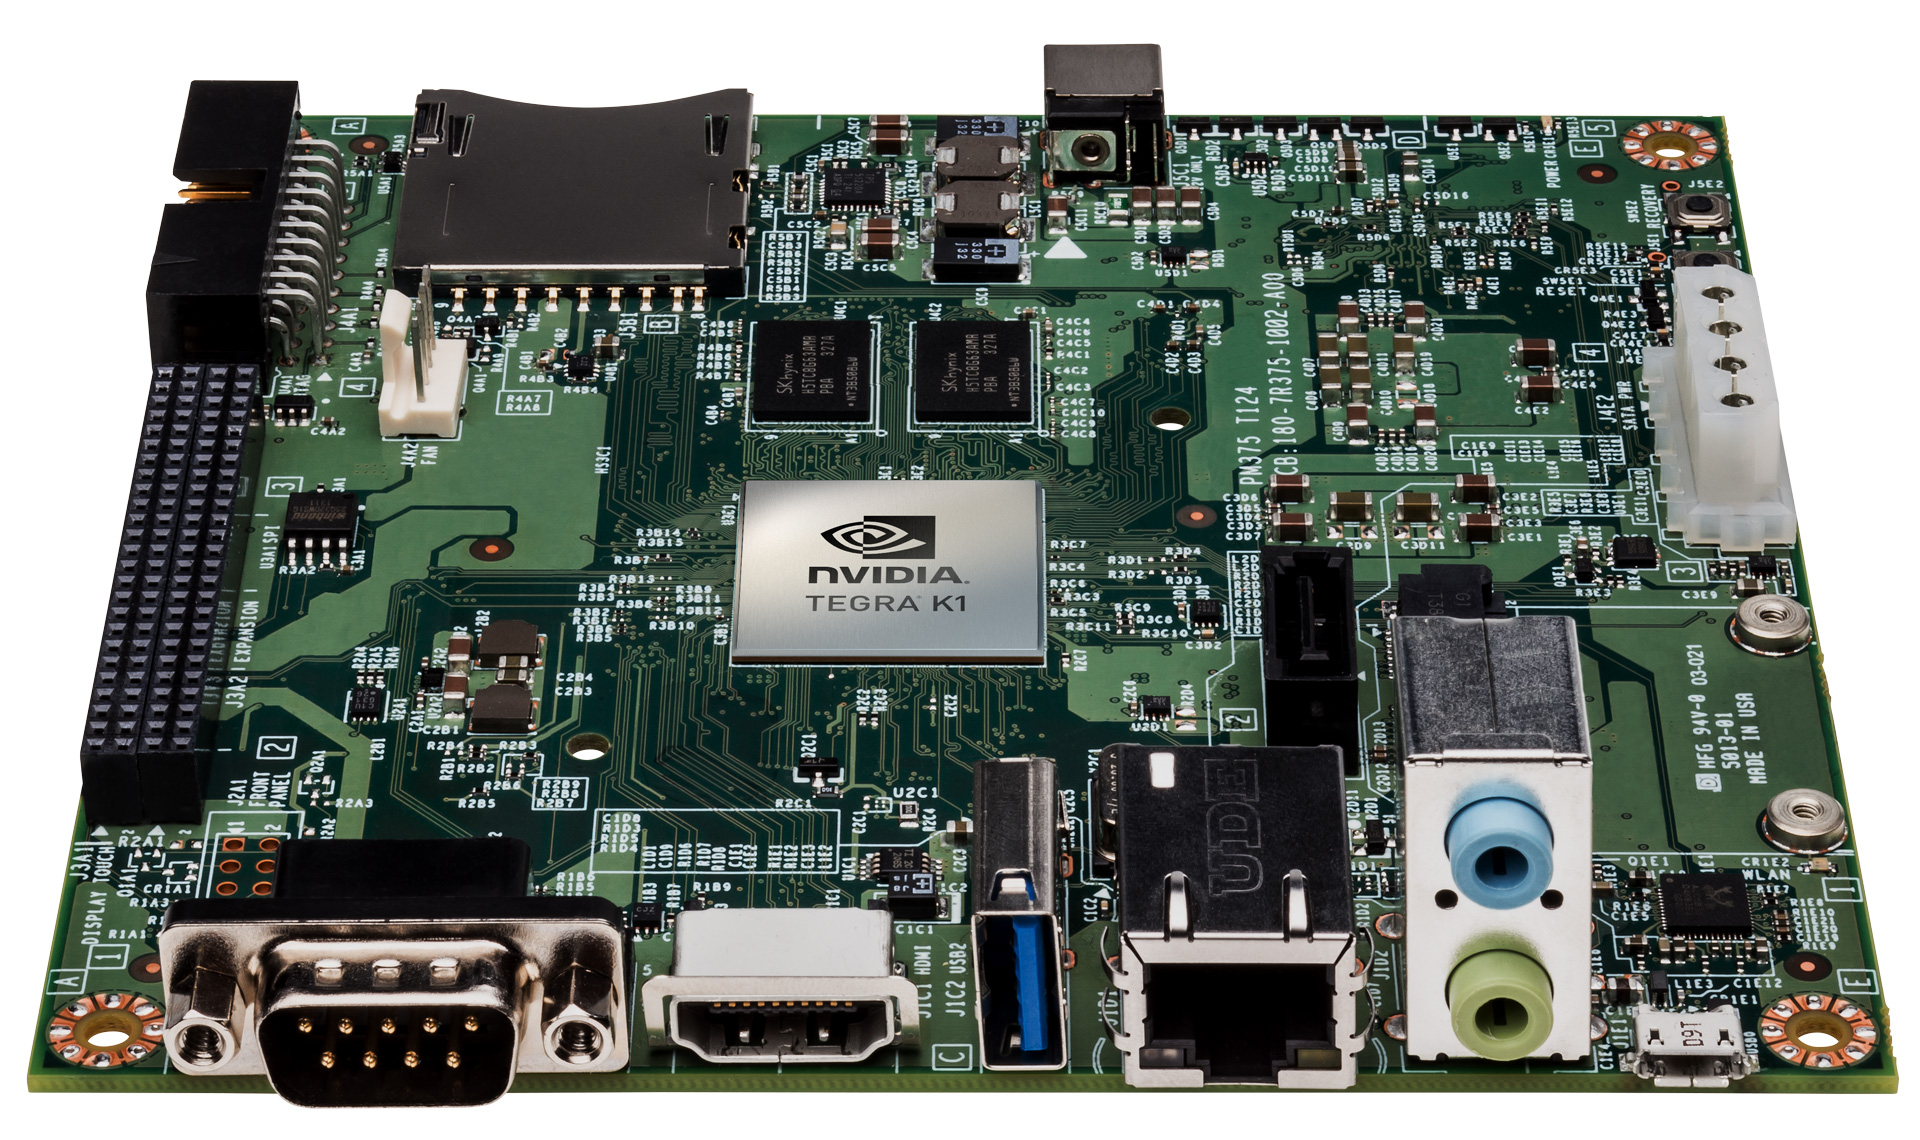
\includegraphics[scale=0.10]{./Resources/jetson_tk1.jpg}
 	\caption{Plataforma de Desenvolvimento - Jetson TK1}
 	\label{jetson_tk1}
\end{figure}

\subsection{Equipamentos auxiliares}

Abaixo estão apresentados os equipamentos auxiliares para o desenvolvimento do trabalho. 

Os métodos para a identificação de correspondências entre as câmeras requerem que a imagem estejam calibradas e retificadas. Por conta disso, utiliza-se o padrão de calibração de dimensão 7x10, apresentado na figura \ref{calibration_pattern}, para este propósito. Deste modo, é possível caracterizar as distorções das lentes, parâmetros intrínsecos, e o posicionamento de uma das câmeras com relação a outra, parâmetros extrínsecos.  

\begin{figure}[H]
 	\centering
 	
\includegraphics[scale=0.10]{./Resources/calibration_pattern.png}
 	\caption{Padrão de Calibração}
 	\label{calibration_pattern}
\end{figure}

A motivação deste trabalho é a sua utilização em veículos aéreos. Por conta disso, é indispensável que se tenha algum desses veículos. O trabalho conta com a utilização de um quadricóptero produzido pela 3DR, porém este apresenta modificações visando o seu desenvolvimento para navegação autônoma. Deste modo, tem-se a adição de \textit{propellers guards}, objetivando o aumento da segurança do veículo e das pessoas que o operam. Além disso, o \textit{drone} conta com suportes para a câmera estereoscópica e para a plataforma embarcada. Como pode ser observado pela figura \ref{quad_camera_support}, todas as peças foram produzidas utilizando impressora 3D.

\begin{figure}[H]
 	\centering
 	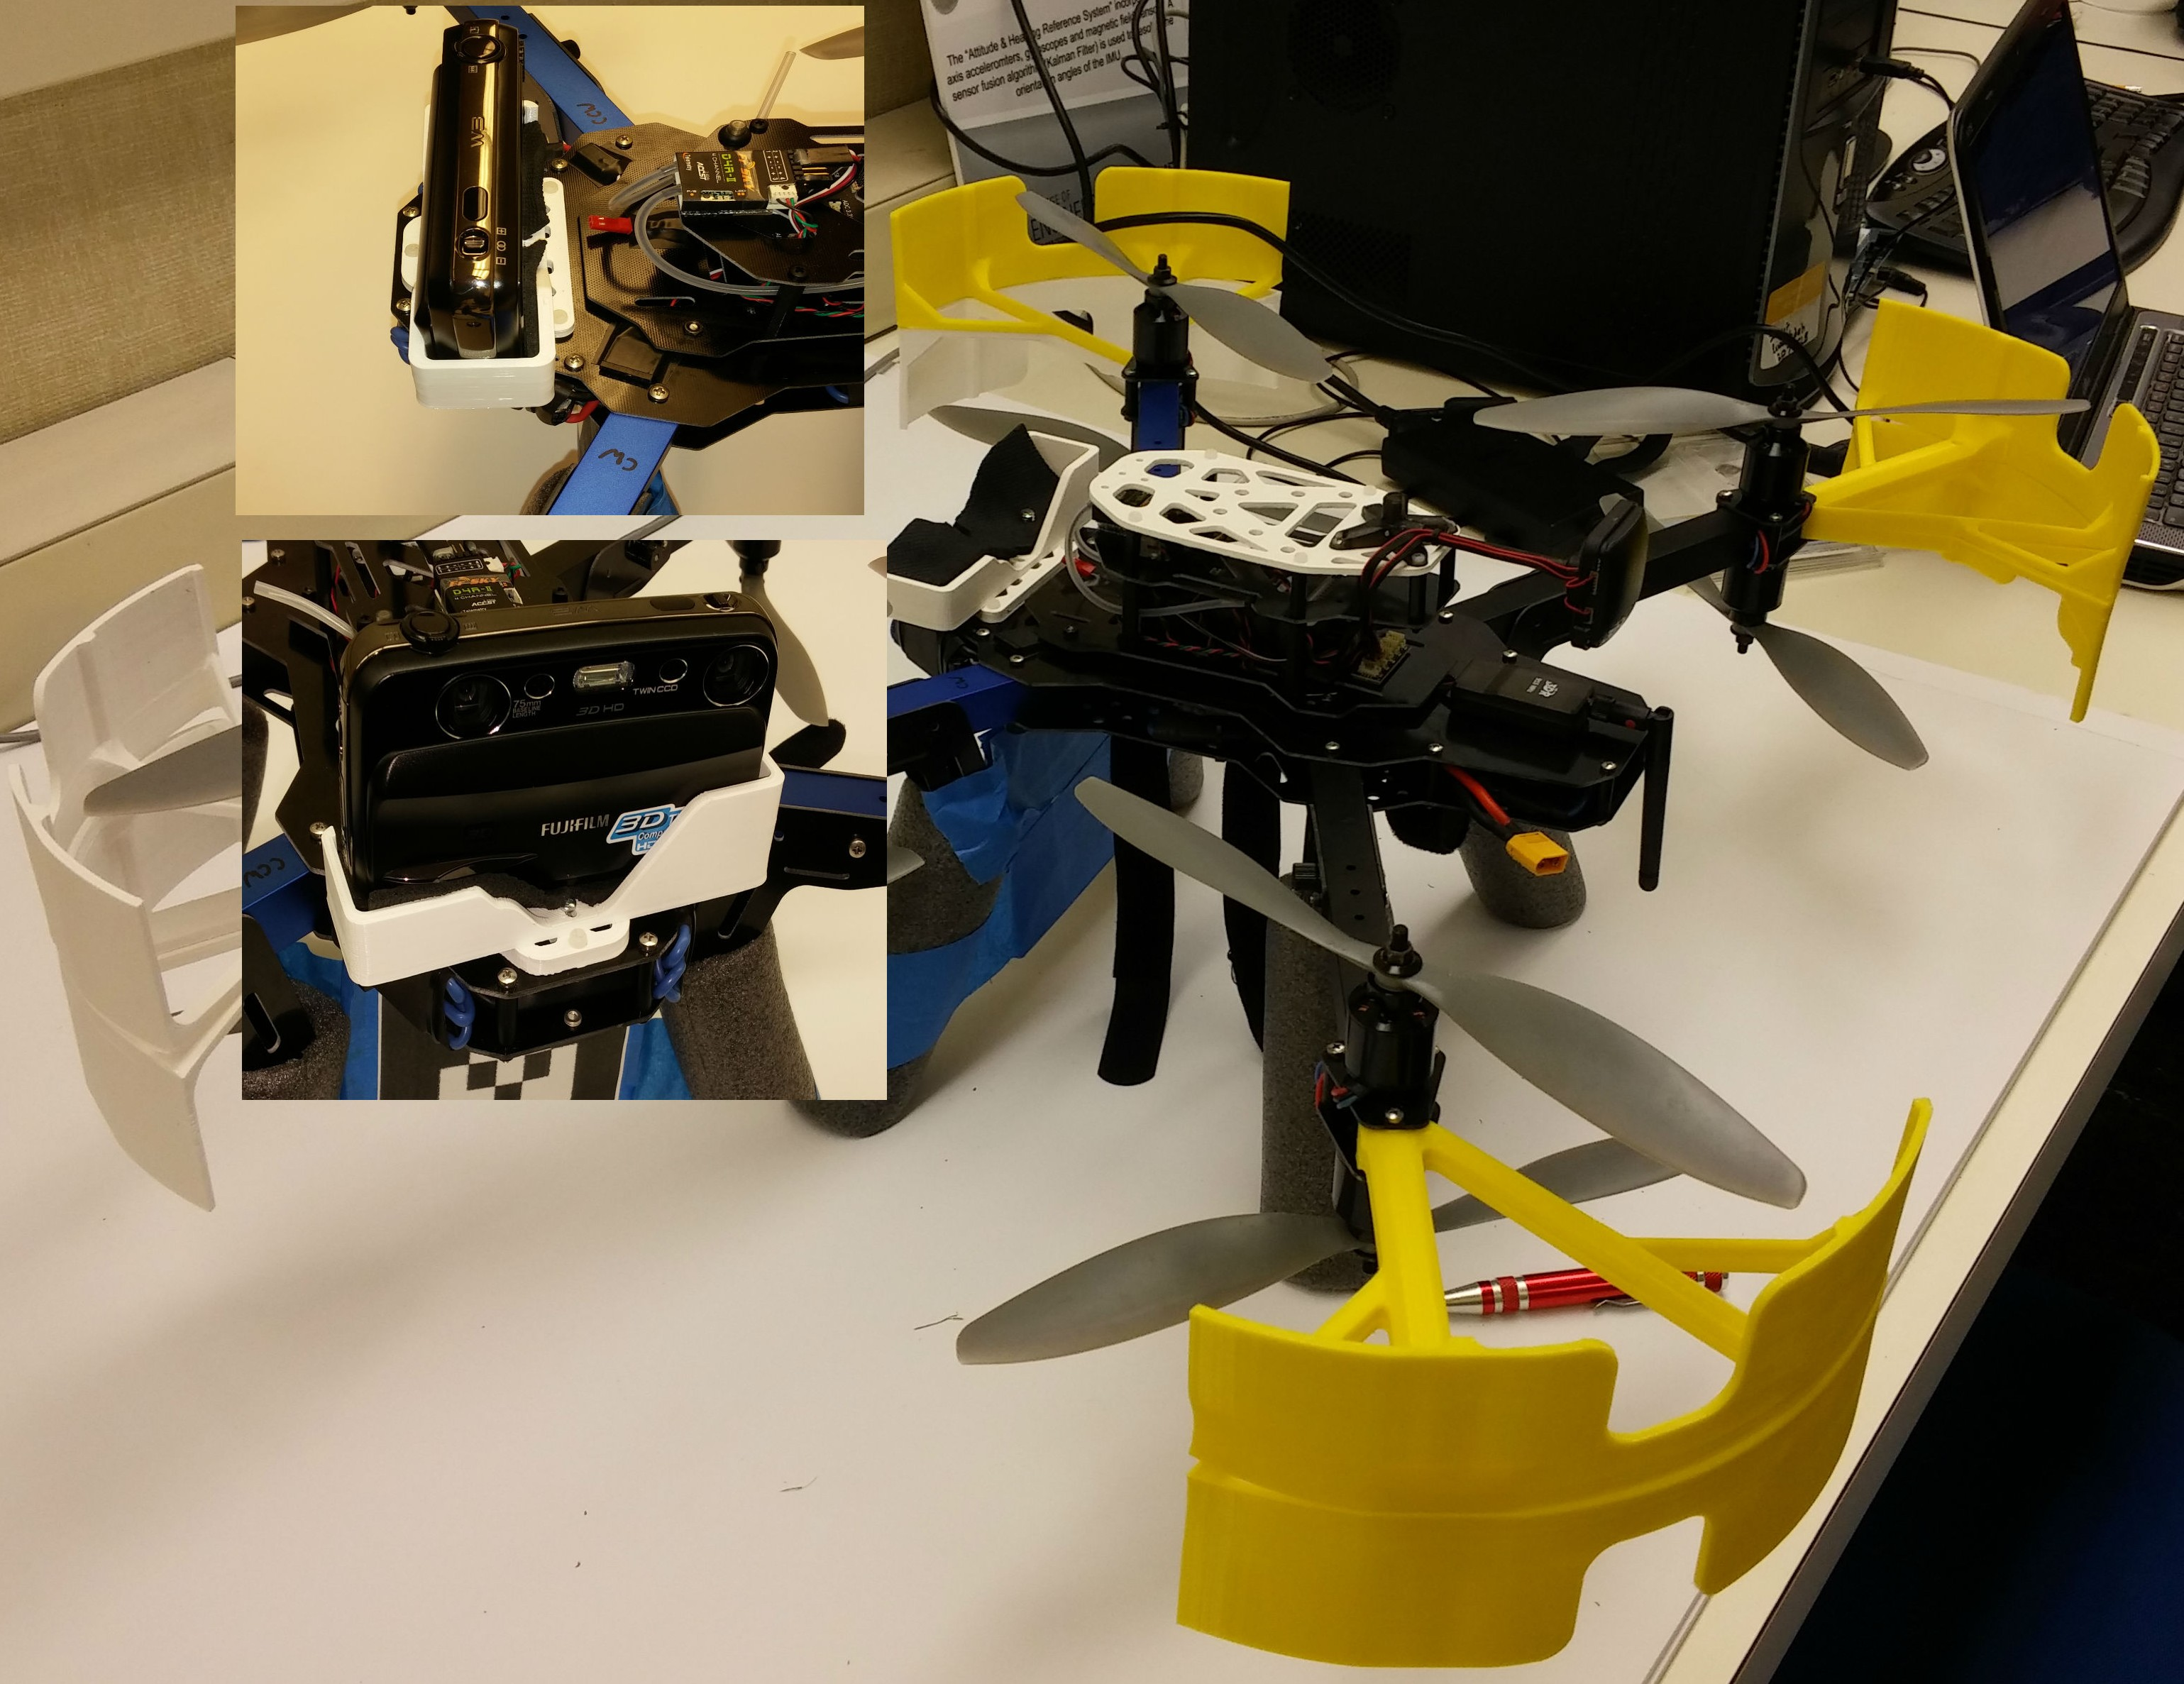
\includegraphics[scale=0.10]{./Resources/quad_camera_support.jpg}
 	\caption{Quadricóptero 3DR X8 com suporte para a Câmera 3D}
 	\label{quad_camera_support}
\end{figure}

%------------------------------------ Métodos -------------------------------------------------------
\section{Métodos}

Nesta seção serão apresentados os cenários e os métodos utilizado para o desenvolvimento do algoritmo para a detecção de obstáculos.

\subsection{Cenários}

O algoritmo de detecção de obstáculos desenvolvido tenta contornar todas as adversidades propostas pelos seguintes cenários. Propôs-se que ele deve ser flexível à variações na luminosidade, capaz de detectar obstáculos estáticos e móveis, e ser imune à vibrações. Deste modo, dois cenários em ambiente confinado e um em ambiente aberto foram analisados. Deseja-se a navegação autônoma ocorra até mesmo em casos que o sinal do Sistema de Posicionamento Global (GPS) seja perdido, por conta disso escolheu-se a utilização dos ambientes confinados. O ambiente externo foi escolhido devido a quantidade de fatores que poderiam atrapalhar e tornar o algoritmo mais robusto.

\subsubsection{Cenário 1}

O cenário da figura \ref{thumb_video10_l} foi utilizado para estudo das condições de ambiente externo, o qual está sujeito grandes variações de luminosidade e um número menor de movimentos, o que permite uma análise de alcances maiores. O principal  obstáculo deste cenário é uma árvore. 

\begin{figure}[H]
 	\centering
 	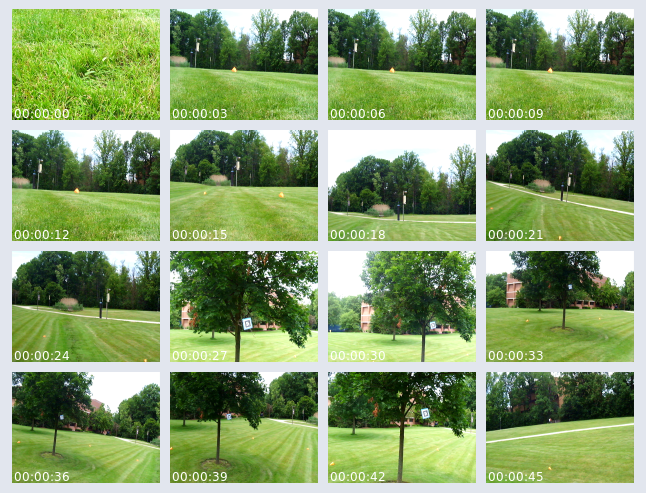
\includegraphics[scale=0.50]{./Resources/thumb_video10_l.png}
 	\caption{Cenário 1 - Ambiente Externo - Árvore}
 	\label{thumb_video10_l}
\end{figure}

\subsubsection{Cenário 2}

O cenário da figura \ref{thumb_video12_l} foi utilizado para estudo das condições de ambiente interno, o qual também apresenta certa variação de luminosidade, porém apresenta um número maior de movimentos, permitindo uma análise de objetos estáticos à curta e média distância. Os principais obstáculos deste cenário são uma mesa, uma cadeira e duas estantes.

\begin{figure}[H]
 	\centering
 	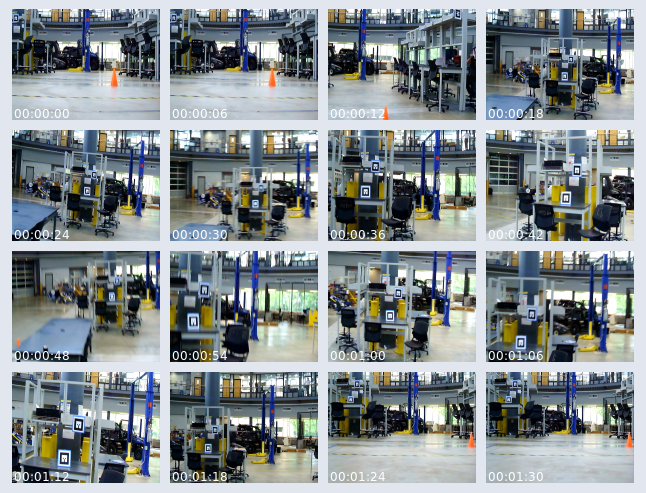
\includegraphics[scale=0.50]{./Resources/thumb_video12_l.png}
 	\caption{Cenário 2 - Ambiente Interno - Mesa/Cadeira/Estantes}
 	\label{thumb_video12_l}
\end{figure}

\subsubsection{Cenário 3}

O cenário da figura \ref{thumb_video15} foi utilizado para estudo das condições de ambiente interno, o qual também apresenta certa variação de luminosidade, apresenta um número muito maior de movimentos e permite a análise de objetos móveis à curto e médio alcance. Os principais obstáculos deste cenário  é uma bancada e um outro quadricóptero no campo de visão do veículo pilotado.

\begin{figure}[H]
 	\centering
 	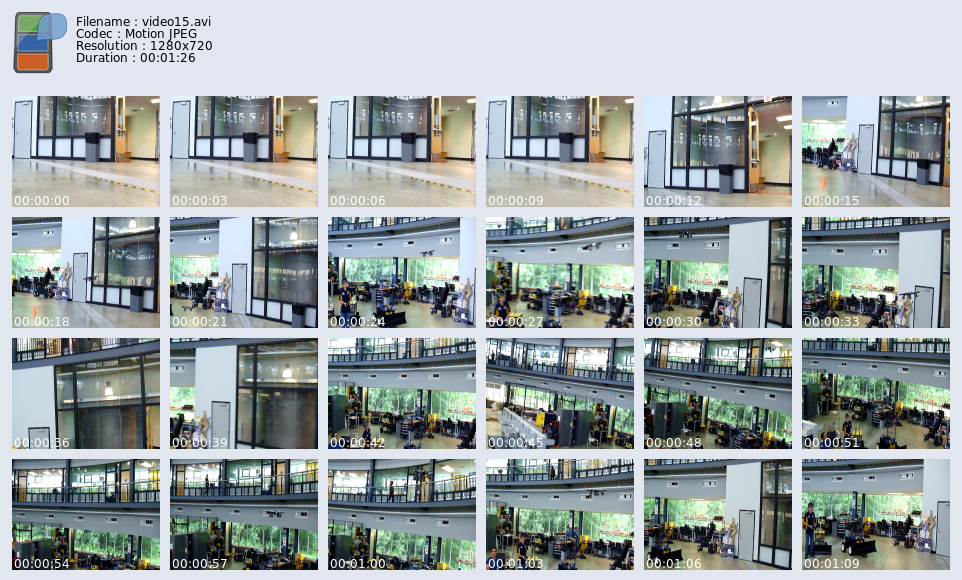
\includegraphics[scale=0.50]{./Resources/thumb_video15.png}
 	\caption{Cenário 3 - Bancada/Quadricóptero}
 	\label{thumb_video15}
\end{figure}


\subsection{Processamento de Imagem}

Nessa seção será apresentado o processamento de imagens utilizado para a identificação de obstáculos. Como pode ser visto na figura \ref{stereo_processor_steps}, todo o processo conta com seis etapas.

\textbf{Câmeras:} O primeiro passo do processo é a captura das imagens da câmera estereoscópica. Idealmente, as imagens deve ser capturadas ao mesmo instante e as lentes não apresentarem distorções.   

\textbf{Calibração e Retificação:} Na prática, as lentes apresentam distorção. Com base nos parâmetros obtidos após a calibração das câmeras é possível retificá-las. 

\textbf{Correspondência Estéreo:} Aplica-se os métodos para encontrar as correspondências entre as duas câmeras, gerando assim o mapa de disparidades.

\textbf{Pré-filtragem:} Este passo, pode ser aplicado tanto nas imagens retificados ou no mapa de disparidades. Atualmente, aplica-se a operação morfológica de abertura e um filtro de Mediana sobre o mapa de disparidades. 

\textbf{Limiarização por Distância:} Visto que a disparidade apresenta uma relação com a distância, aplica-se uma operação de limiarização. Deste modo, apenas os obstáculos a uma certa distância são segmentados.

\textbf{Identificação de Obstáculos:} Após o passo anterior, o objeto é identificado e sua posição é rastreada. Essa informação pode ser utilizada pelo sistema de controle da aeronave para manter distância do obstáculo identificado.

\begin{figure}[H]
 	\centering
 	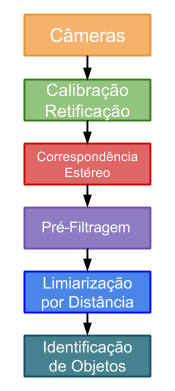
\includegraphics[scale=0.50]{./Resources/stereo_processor_steps.png}
 	\caption{Etapas do Processamento de Imagens}
 	\label{stereo_processor_steps}
\end{figure}

%\subsection{Métodos Estéreo }
%
%\subsubsection{Método Estéreo Local - \textit{Block Matching}}
%
%\subsubsection{Método Estéreo Semi-global - \textit{Semi-global Block Matching}}

%-----------------------------------------------------------------------------------------------------------------------------------------------------------------------------------------------
% Resultados/Discussões: 
% Aqui se mostra o que o trabalho permitiu produzir, e às vezes o que pode ser comparado com outros trabalhos
% Aqui ficam claras se as propostas do trabalho são relevantes ou não, pois devem permitir a discussão do trabalho;
% Deve-se responder: Os resultados estão claros em bom número (nem muito nem pouco) que permitam avaliar realmente a proposta e o que foi produzido.
\chapter{Resultados}
\label{Resultados}

Os resultados apresentados neste capítulo estão divididos em duas partes. Os resultados da seção \ref{resultsGUI} estão inteiramente relacionados as funções fundamentais presentes na interface gráfica desenvolvida. Já na seção \ref{resultsComparison}, tem-se presente os resultados que apresentam os dados obtidos através dos testes de desempenho dos métodos de \textit{Stereo Matching} nas plataformas utilizadas.

%-----------------------------------------------------------------------------------------------------------------------------------------------------------------------------------------------
\section{Interface Gráfica - \textit{StereoVisionGUI}}
\label{resultsGUI}

Nesta seção, o software desenvolvido apresenta uma interface gráfica (GUI -- \textit{Graphical User Interface}) amigável, a qual facilita a visualização das imagens da câmera estéreo, 
dos mapas de disparidades, da reconstrução tridimensional e do método de processamento de imagens desenvolvido. Atualmente, o software conta com três métodos para encontrar correspondências 
estéreo (BM, SGBM e BMGPU) e com 8 opções das quais 6 delas são destinadas a visualização das seguintes perspectivas:

\begin{enumerate}
  \item Imagens retificadas das câmeras esquerda e direita
  \item Mapa de disparidades em Escala de Cinza e RGB
  \item Mapa tridimensional do ambiente reconstruído em Escala de Cinza e RGB
  \item Imagem da Câmera Esquerda com o indicador de objeto rastreado e Imagem binária resultante da limiarização por distância.
  \item Imagem resultante do processo de detecção de movimentos e Imagem resultante do processo de detecção de movimentos limiarizada por distância. 
  \item Imagem resultante da adição da imagem à direita com a Imagem da Câmera Esquerda e Imagem resultante do processo de realce das bordas dos objetos em movimento próximos ao veículo.
\end{enumerate} 

O botão \textit{Show Left/Right} seleciona a opção na qual a interface gráfica permite a visualização simultânea das imagens retificadas de ambas câmera. A figura \ref{gui_showleftright_view} 
ilustra o comportamento do software quando essa opção é selecionada. 

O botão \textit{Show Disparity Map} seleciona a opção na qual a interface gráfica permite a visualização simultânea dos mapas de disparidade em escala de cinza e RGB. A figura 
\ref{gui_showdisparitymap_view} ilustra o comportamento do software quando essa opção é selecionada. 

O botão \textit{Show 3D Reconstruction} seleciona a opção na qual a interface gráfica permite a visualização simultânea dos mapas tridimensionais do ambiente reconstruído em escala de cinza e 
RGB. A figura \ref{gui_show3dreconstruction_view} ilustra o comportamento do software quando essa opção é selecionada. 

O botão \textit{Show Tracking Object View} seleciona a opção na qual a interface gráfica permite a visualização simultânea da imagem da câmera Esquerda com o indicador de objeto rastreado e 
imagem binária resultante da limiarização por distância. A figura \ref{gui_show_tracking_object_view} ilustra o comportamento do software quando essa opção é selecionada. 

O botão \textit{Show DiffImage} seleciona a opção na qual a interface gráfica permite a visualização simultânea da imagem resultante do processo de detecção de movimentos e imagem resultante do 
processo de detecção de movimentos limiarizada por distância. A figura \ref{gui_showdiffimage_view} ilustra o comportamento do software quando essa opção é selecionada. 

O botão \textit{Show Warning Edges} seleciona a opção na qual a interface gráfica permite a visualização simultânea da imagem resultante da adição da imagem à direita com a imagem da câmera esquerda e imagem resultante do processo de realce das bordas dos objetos em movimento próximos ao veículo. A figura \ref{gui_showwarningedges_view} ilustra o comportamento do software quando essa opção é selecionada. 


\begin{figure}[H]
 	\centering
 	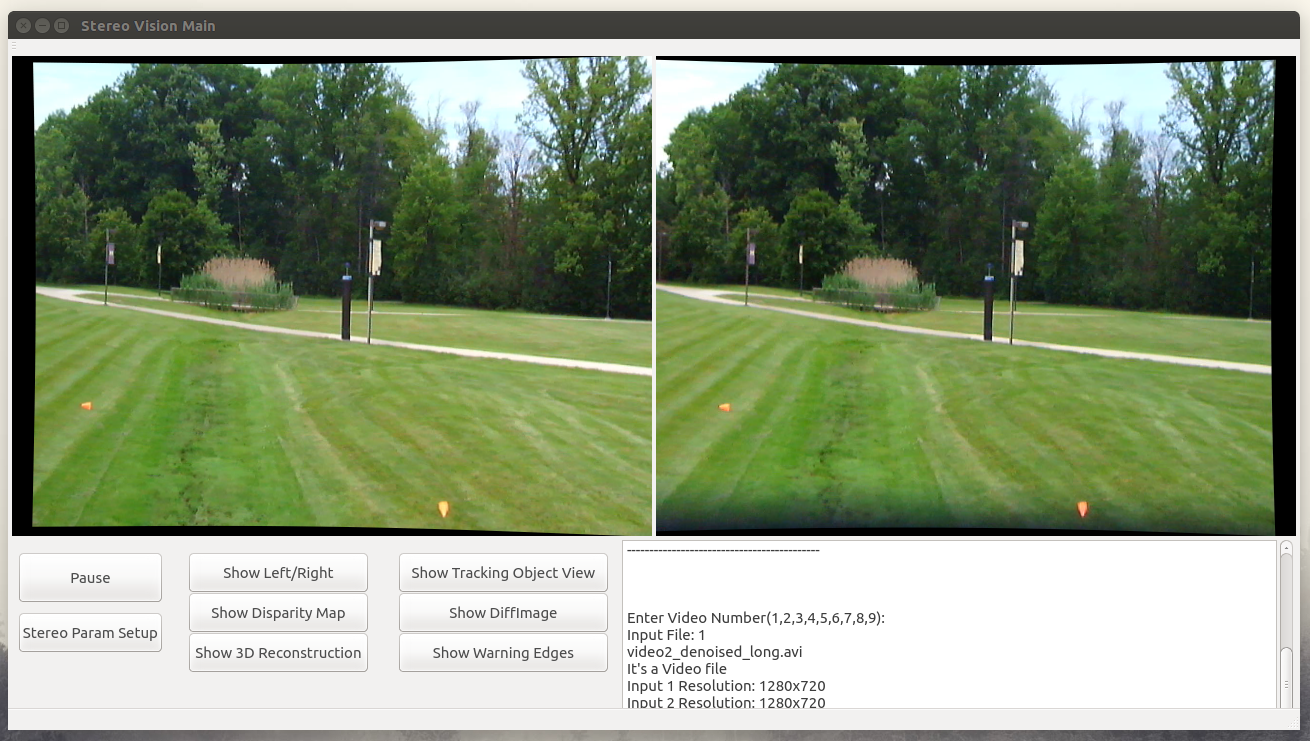
\includegraphics[scale=0.35]{./Resources/gui_showleftright_view.png}
 	\caption{Interface Gráfica - Visualização simultânea dos quadros das câmeras esquerda e direita}
 	\label{gui_showleftright_view}
\end{figure}


\begin{figure}[H]
 	\centering
 	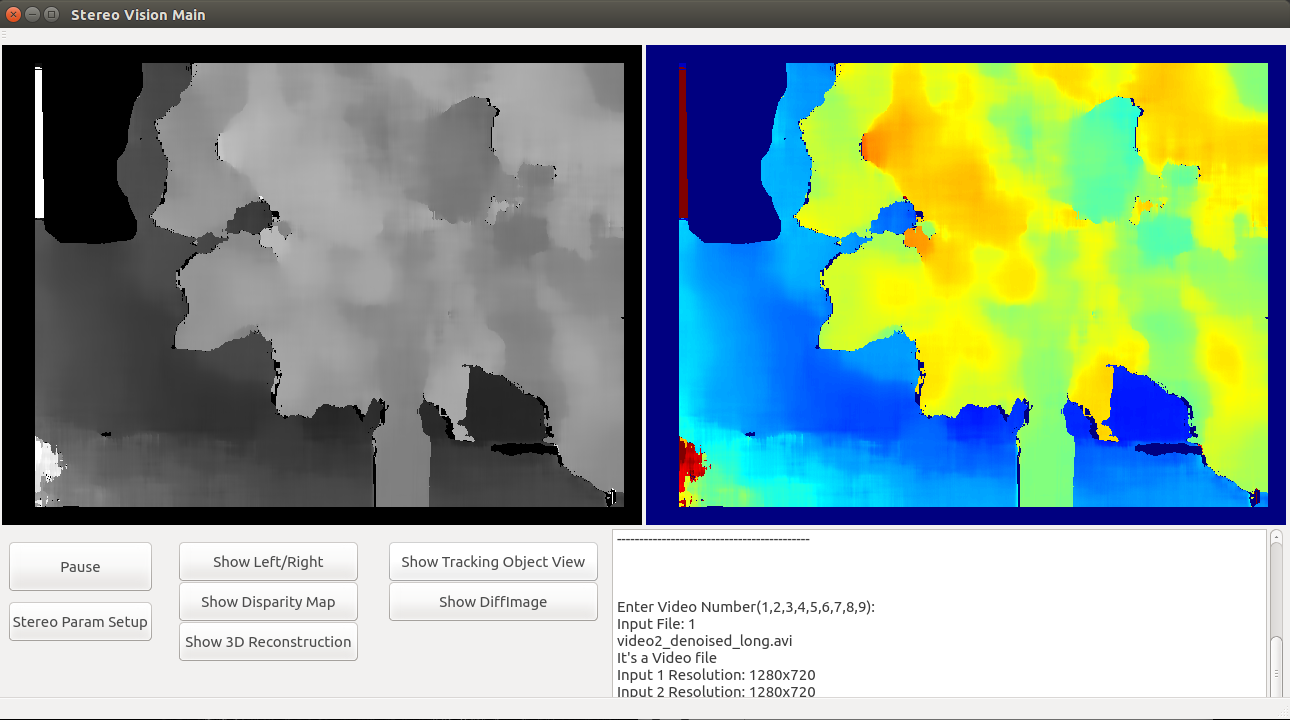
\includegraphics[scale=0.35]{./Resources/gui_showdisparitymap_view.png}
 	\caption{Interface Gráfica - Visualização dos Mapa de disparidades em Escala de Cinza e RGB}
 	\label{gui_showdisparitymap_view}
\end{figure}


\begin{figure}[H]
 	\centering
 	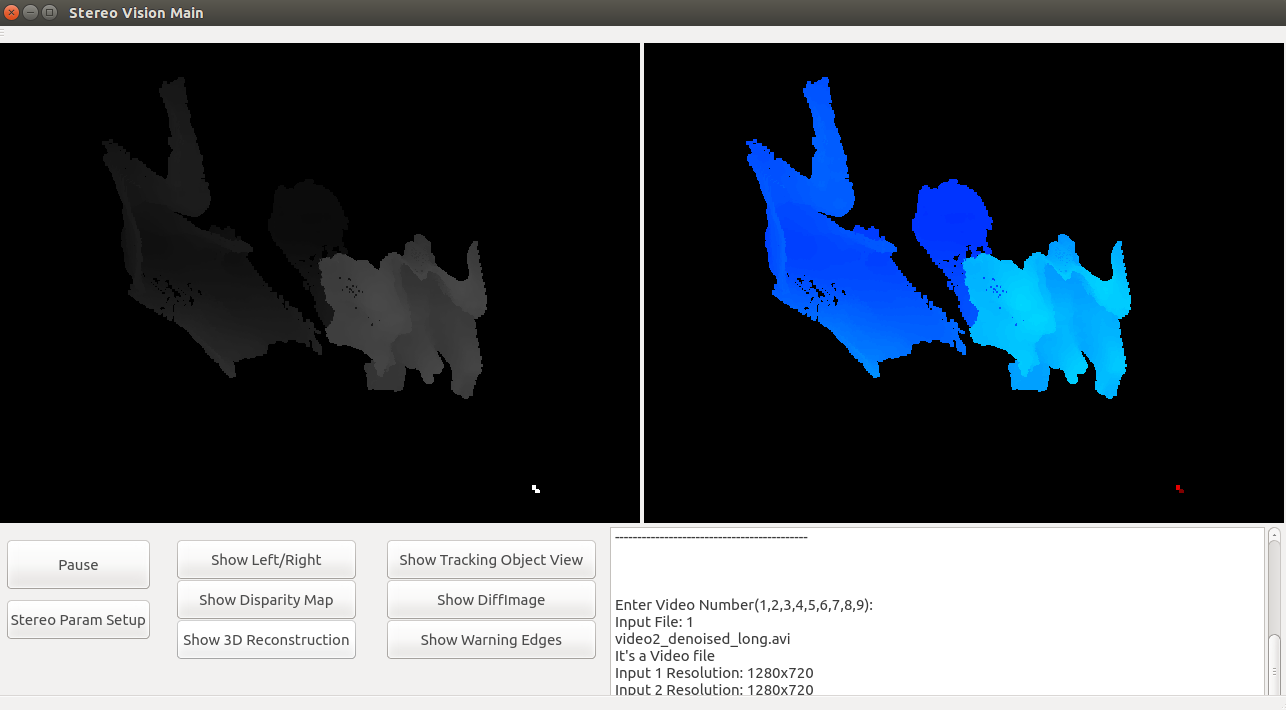
\includegraphics[scale=0.35]{./Resources/gui_show3dreconstruction_view.png}
 	\caption{Interface Gráfica - Visualização dos Mapa de disparidades em Escala de Cinza e RGB}
 	\label{gui_show3dreconstruction_view}
\end{figure}


\begin{figure}[H]
 	\centering
 	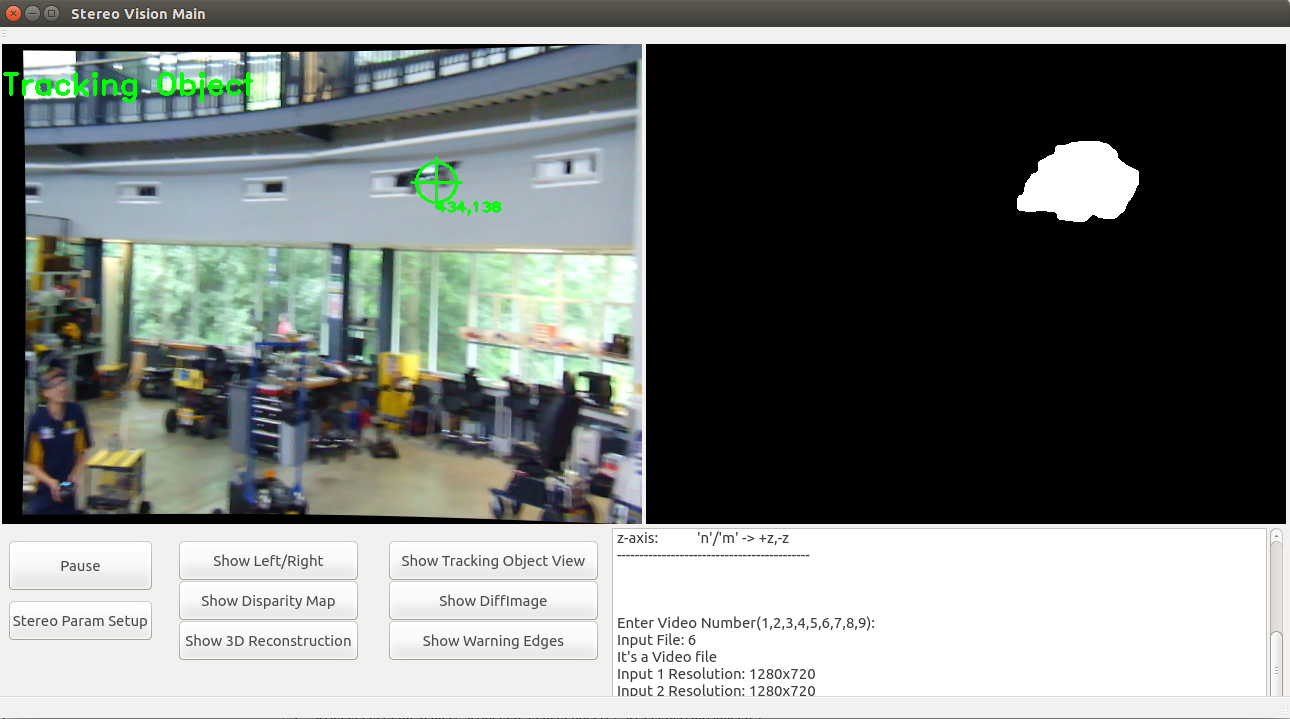
\includegraphics[scale=0.35]{./Resources/gui_show_tracking_object_view.png}
 	\caption{Interface Gráfica - Visualização da Imagem da Câmera Esquerda com o indicador de objeto rastreado e da Imagem binária resultante da limiarização por distância}
 	\label{gui_show_tracking_object_view}
\end{figure}


\begin{figure}[H]
 	\centering
 	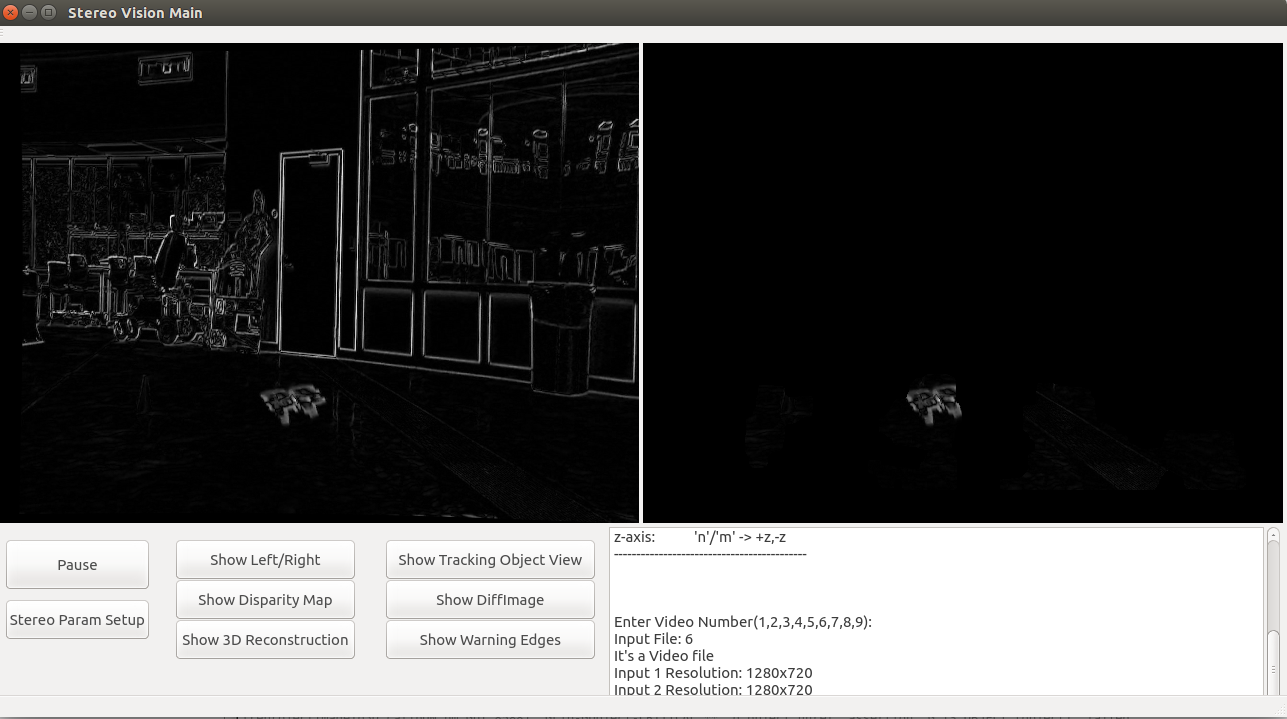
\includegraphics[scale=0.35]{./Resources/gui_showdiffimage_view.png}
 	\caption{Interface Gráfica - Visualização da imagem resultante do processo de detecção de movimentos e imagem resultante do processo de detecção de movimentos limiarizada por distância}
 	\label{gui_showdiffimage_view}
\end{figure}


\begin{figure}[H]
 	\centering
 	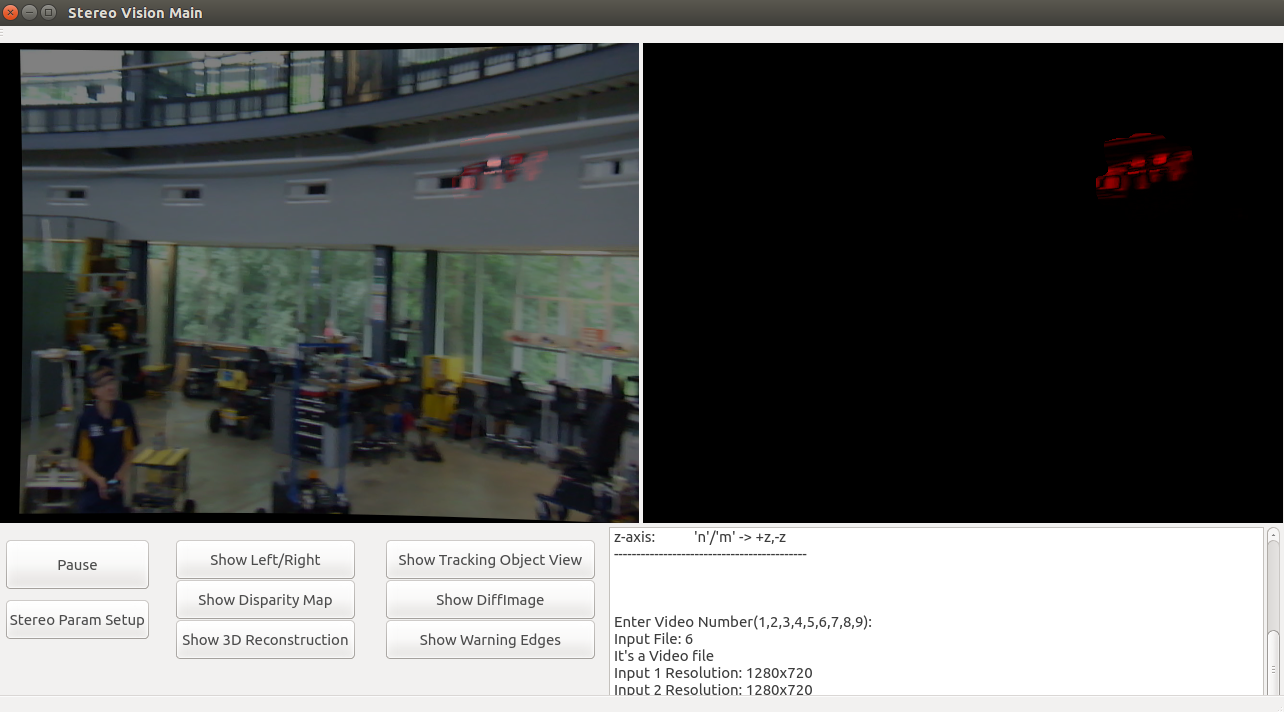
\includegraphics[scale=0.35]{./Resources/gui_showwarningedges_view.png}
 	\caption{Interface Gráfica - Visualização da Imagem resultante da adição da imagem à direita com a Imagem da Câmera Esquerda e Imagem resultante do processo de realce das bordas dos 
 	objetos em movimento próximos ao veículo}
 	\label{gui_showwarningedges_view}
\end{figure}

% TODO: Colocar Novas Imagens com os resultados mais bonitos. Tirar fotos de uma mesma cena comparativamente ao 3 métodos


%-----------------------------------------------------------------------------------------------------------------------------------------------------------------------------------------------
\section{Comparação de Desempenho: Desktop x BBB x Jetson TK1}
\label{resultsComparison}

Nesta seção, estão apresentados os resultados práticos das diferentes implementações dos métodos de visão estéreo nas plataformas abordadas. Os Métodos utilizados foram BM, SGBM e BMGPU para a comparação das plataformas. O método BMGPU mostrou-se o de melhor performance, visto que é o que requisita menor processamento dentre os outros métodos mais conhecidos (SGBM, BP, CSBP, AD Census, ...) além de ser acelerado em hardware. A tabela \ref{resultsCPUGPU} abaixo, apresenta o resultado de desempenhos obtidos nas plataformas, apresentando comparativamente seu desempenho quando o processado utilizando CPU ou GPU/NEON (Caso da BBB). Com relação à configuração utilizada para a realização dos teste, utilizou-se uma resolução de 640x480, um tamanho média da janela usada para combinar blocos de pixels (\textit{SADWindowSize}) de 15 e um tamanho da gama de disparidades (\textit{NumberOfDisparities}) igual à 16, como pode ser observado na tabela \ref{teste_values}. O critério de escolha desses valores foi dado pelo balanço entre performance e qualidade do mapa de disparidades gerado, isto é, um mapa que fosse denso (confiável) e permitisse a identificação correta dos obstáculos.

\begin{table}[]
\centering
\caption{Configuração utilizada para Avaliação de Performance}
\label{teste_values}
\begin{tabular}{|c|c|}
\hline
                    & Configuração \\ \hline
Resolução           & 640x480      \\ \hline
SADWindowSize       & 15           \\ \hline
NumberOfDisparities & 16           \\ \hline
\end{tabular}
\end{table}

\begin{table}[]
\centering
\caption{Desempenho atingido por cada plataforma dos Métodos Utilizados}
\label{resultsCPUGPU}
\begin{tabular}{|c|c|c|c|}
\hline
FPS       & BM & SGBM & BM\_GPU  \\ \hline
Desktop   & 28 & 12   & 30       \\ \hline
BBB       & 1  & -    & -        \\ \hline
JetsonTK1 & 6  & 2    & 7$\sim$8 \\ \hline
\end{tabular}
\end{table}

\begin{figure}[H]
 	\centering
 	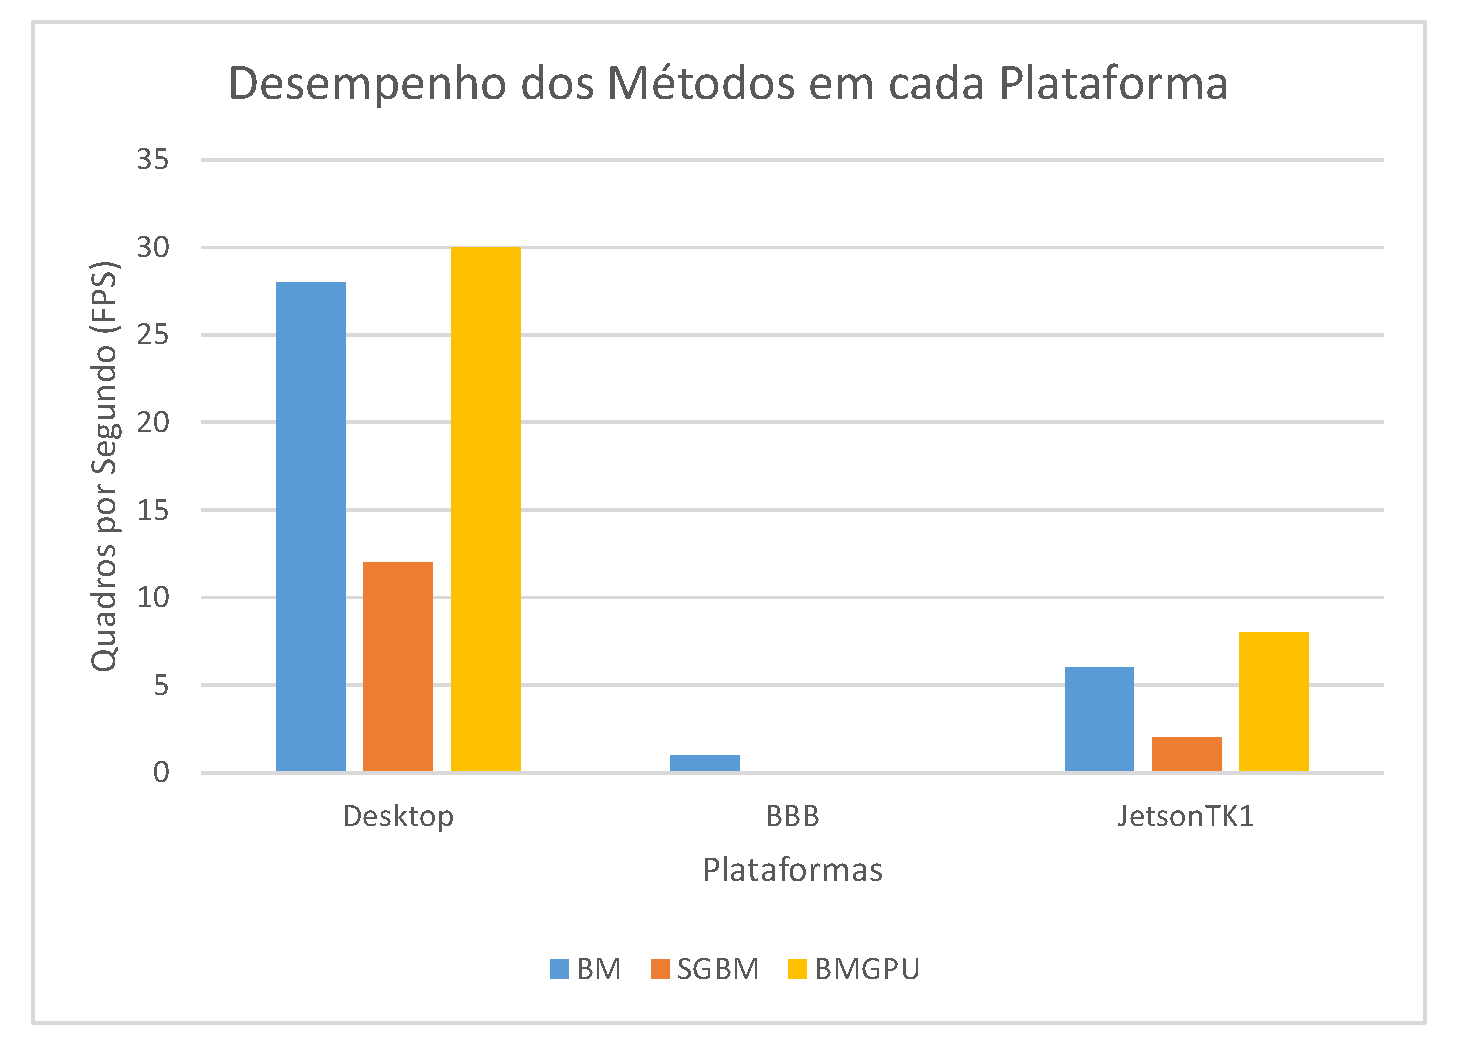
\includegraphics[scale=0.5]{./Resources/grafico_desempenho.pdf}
 	\caption{Gráfico - Comparação de Desempenho dos Métodos Estéreos para cada plataforma.}
 	\label{grafico_desempenho}
\end{figure}

%-----------------------------------------------------------------------------------------------------------------------------------------------------------------------------------------------
\subsection{Desktop}
\subsubsection{CPU}
\subsubsection{GPU}


%-----------------------------------------------------------------------------------------------------------------------------------------------------------------------------------------------
\subsection{BeagleBone Black(BBB)}
\subsubsection{CPU}
\subsubsection{NEON}


%-----------------------------------------------------------------------------------------------------------------------------------------------------------------------------------------------
\subsection{Jetson TK1}
\subsubsection{CPU}
\subsubsection{GPU}
%-----------------------------------------------------------------------------------------------------------------------------------------------------------------------------------------------
% Conclusões: "fecha" com os objetivos? (respondem aos objetivos?) - aqui é que "se vende o peixe" - elas é que valorizam (ou não) o trabalho realizado.
% Normalmente é uma parte do trabalho "um pouco desprezada", pois o autor já está "cansado....". Mas é aqui que realmente se mede se o trabalho tem ou não valor.
% Contém o item Trabalhos futuros, que é uma orientação sobre as possibilidades de continuação do desenvolvimento do trabalho.
\chapter{Conclusão}
\label{Conclusao}

Acredita-se que o trabalho desenvolvido até então está em dia com o cronograma, visto que a interface gráfica desenvolvida encontra-se totalmente funcional e o algoritmo detecta e segmenta relativamente bem os obstáculos dos cenários propostos. Entretanto, a taxa de processamento tornou-se uma preocupação, visto que o algoritmo desenvolvido consegue processar a uma taxa de captura de aproximadamente oito quadros por segundo. A alteração de plataforma poderia ser uma solução para o aumento da taxa de atualização, visto que o código implementado nos sistema embarcados dispensam interface gráfica e diversas outras funcionalidades, como exemplo a funcionalidade para reconstrução tridimensional do ambiente. Todavia, essas plataformas não são tão poderosas quanto o computador da estação-base, logo, possivelmente essas plataformas apresentem performance inferior.

Deste modo, duas providencias  são cruciais para a continuidade do trabalho. A primeira é a otimização das rotinas utilizadas pelo algoritmo, sendo essa uma tentativa para a melhora do desempenho geral do método. A segunda é a execução de uma ampla revisão bibliográfica, incluindo principalmente trabalhos que apresentem comparativos de desempenho entre plataformas e que tenham realizados algum tipo de aceleração por \textit{hardware}, sejam eles envolvendo paralelização de processos, implementação em FPGA ou utilizando a plataforma de computação paralela CUDA (\textit{Compute Unified Device Architecture}). Deste modo, será possível identificar a plataforma mais adequada para este propósito. 

Atividades Futuras:

\begin{itemize}
	\item Otimizar Código
	\item Alterar Interface gráfica para suportar o Método SGBM
	\item Implementar Segmentação por Distância/Limiarização do mapa de disparidades utilizando Método de Otsu
	\item Aprimorar a suavização da Nuvem de Pontos Gerada
	\item Analisar Métodos de Abertura e Fechamento para aprimoramento na Segmentação
	\item Implementar funções para medir a Distância de objetos próximos
	\item Reavaliar a Calibração das Câmeras	
	\item Realizar ensaio de Ground Truth para validação da Distância Detectada
	\item Implementar os algoritmos de Visão na BeagleBone e Jetson TK1
	\item Implementar os algoritmos de Visão na Jetson TK1
	\item Comparação de Desempenho: Desktop x BBB x Jetson TK1
\end{itemize}









%------------------------------------- ADI��O DAS BIBLIOGRAFIAS -------------------------------------	
\bibliographystyle{unsrt} 			% Define o estilo da bibliografia
\bibliography{./Content/References} 	% Faz refer�ncia ao arquivo ref.bib

%------------------------------------- Configura��es de Anexos --------------------------------------
\newcommand{\annexname}{Anexo}
\makeatletter
\newcommand\annex{\par
  \setcounter{chapter}{0}%
  \setcounter{section}{0}%
  \gdef\@chapapp{\annexname}%
  \gdef\thechapter{\@Roman\c@chapter}}
\makeatother

\newenvironment{poliabstract}[1]
  {\renewcommand{\abstractname}{#1}\begin{abstract}}
  {\end{abstract}}

%------------------------------------- Adi��o dos Anexos -------------------------------------------- 	
%\begin{appendices}
\appendix
%------------------------------------- Ap�ndice 1  --------------------------------------------------
\chapter{Ap�ndice 1}
\label{Apendice1}

%%Remover
%\textcolor{red}{\textbf{Dica:} Diferen�a entre Ap�ndice e Anexo:
%	\begin{itemize}
%		\item AP�NDICE -- Documento ou texto elaborado pelo autor
%		\item ANEXO -- Documento ou texto n�o elaborado pelo autor
%	\end{itemize}
%}

Abaixo est�o apresentados todos os trechos de c�digo desenvolvido para este trabalho. Essa se��o est� subdividada organizada em duas partes, bibliotecas e c�digo-fonte, para cada uma das plataformas utilizadas.

\section{Interface Gr�fica - StereoVision System}
\subsection{Bibliotecas}

\lstset{language=C++}
\textbf{3DReconstruction.h}
\begin{lstlisting}
/*
 * 3DReconstruction.h
 *
 *  Created on: Oct 25, 2015
 *      Author: nicolasrosa
 */

#ifndef RECONSTRUCTION_3D_H
#define RECONSTRUCTION_3D_H

/* Libraries */
#include "opencv2/opencv.hpp"

using namespace cv;
using namespace std;

/* 3D Reconstruction Classes */
template <class T>
static void projectImagefromXYZ_(Mat& image, Mat& destimage, Mat& disp, Mat& destdisp, Mat& xyz, Mat& R, Mat& t, Mat& K, Mat& dist, Mat& mask, bool isSub);

template <class T>
static void fillOcclusionInv_(Mat& src, T invalidvalue);

template <class T>
static void fillOcclusion_(Mat& src, T invalidvalue);

// 3D Reconstruction
class Reconstruction3D{
public:
    Reconstruction3D(); //Constructor
    void setViewPoint(double x,double y,double z);
    void setLookAtPoint(double x,double y,double z);
    void PointCloudInit(double baseline,bool isSub);

    /* 3D Reconstruction Functions */
    void eular2rot(double yaw,double pitch, double roll,Mat& dest);
    void lookat(Point3d from, Point3d to, Mat& destR);
    void projectImagefromXYZ(Mat &image, Mat &destimage, Mat &disp, Mat &destdisp, Mat &xyz, Mat &R, Mat &t, Mat &K, Mat &dist, bool isSub);
    void fillOcclusion(Mat& src, int invalidvalue, bool isInv);


    Mat disp3Dviewer;
    Mat disp3D;
    Mat disp3D_8U;
    Mat disp3D_BGR;

    Point3d viewpoint;
    Point3d lookatpoint;


    Mat dist;
    Mat Rotation;
    Mat t;

    Mat depth;

    double step;
    bool isSub;
};


#endif // RECONSTRUCTION_3D_H
\end{lstlisting}

\textbf{mainwindow.h}
\begin{lstlisting}
/*
 * mainwindow.h
 *
 *  Created on: Oct 1, 2015
 *      Author: nicolasrosa
 */

#ifndef MAINWINDOW_H
#define MAINWINDOW_H

/* Libraries */
#include <QMainWindow>
#include <opencv2/opencv.hpp>

/* Custom Libraries */
#include "StereoProcessor.h"
#include "setstereoparams.h"

using namespace cv;

namespace Ui{
    class MainWindow;
}

class MainWindow : public QMainWindow{
    Q_OBJECT

public:
    explicit MainWindow(QWidget *parent = 0);
    void StereoVisionProcessInit();
    void printHelp();
    void openStereoSource(int inputNum);
    void createTrackbars();
    QImage putImage(const Mat& mat);
    ~MainWindow();

private:
    Ui::MainWindow *ui;
    StereoProcessor *stereo;
    SetStereoParams *stereoParamsSetupWindow;

    QImage qimageL,qimageR;

    QTimer* tmrTimer;

public slots:
    void StereoVisionProcessAndUpdateGUI();

private slots:
    void on_btnPauseOrResume_clicked();
    void on_btnShowDisparityMap_clicked();
    void on_btnShowStereoParamSetup_clicked();
    void on_btnShow3DReconstruction_clicked();
    void on_btnShowInputImages_clicked();
    void on_btnShowTrackingObjectView_clicked();
    void on_btnShowDiffImage_clicked();
    void on_btnShowDiffImage_2_clicked();
};

#endif // MAINWINDOW_H
\end{lstlisting}

\textbf{reprojectImageTo3D.h}
\begin{lstlisting}
/*
 * reprojectImageTo3D.h
 *
 *  Created on: Jun 18, 2015
 *      Author: nicolasrosa
 */

#ifndef reproject_Image_To_3D_LIB_H_
#define reproject_Image_To_3D_LIB_H_

/* Libraries */
#include <opencv2/opencv.hpp>
#include <fstream>

using namespace cv;

/* Calibration */
#define RESOLUTION_640x480
//#define RESOLUTION_1280x720
#define CALIBRATION_ON

/* Functions Scope */
void on_trackbar(int,void*);

void imageProcessing1(Mat img, Mat imgMedian, Mat imgMedianBGR);
void imageProcessing2(Mat src, Mat imgE, Mat imgED,Mat cameraFeedL,bool isTrackingObjects);

void resizeFrames(Mat* frame1,Mat* frame2);
void changeResolution(VideoCapture* cap_l,VideoCapture* cap_r);
void contrast_and_brightness(Mat &left,Mat &right,float alpha,float beta);

/* Global Variables */
bool isVideoFile=false;
bool isImageFile=false;
bool needCalibration=false;
bool isStereoParamSetupTrackbarsCreated=false;
bool isTrackingObjects=true;

#endif /* reproject_Image_To_3D_LIB_H_ */
\end{lstlisting}

\textbf{setstereoparams.h}
\begin{lstlisting}
/*
 * setstereoparams.h
 *
 *  Created on: Oct 1, 2015
 *      Author: nicolasrosa
 */

#ifndef SETSTEREOPARAMS_H
#define SETSTEREOPARAMS_H

#include <QDialog>

class StereoProcessor; // forward-declaration

namespace Ui {
    class SetStereoParams;
}

class SetStereoParams : public QDialog{
    Q_OBJECT

public:
    explicit SetStereoParams(QWidget *parent = 0, StereoProcessor *stereo = 0);
    void loadStereoParamsUi(int preFilterSize,int preFilterCap,int SADWindowSize,int minDisparity,int numberOfDisparities,int textureThreshold,int uniquenessRatio, int speckleWindowSize, int speckleRange,int disp12MaxDiff);

    ~SetStereoParams();

    bool isAlreadyShowing;

signals:
    void valuesChanged(int preFilterSize, int preFilterCap, int sadWindowSize, int minDisparity, int numOfDisparities, int textureThreshold, int uniquenessRatio, int speckleWindowSize, int speckleWindowRange, int disp12MaxDiff);
private slots:
    /* Sliders */
    void on_preFilterSize_slider_valueChanged(int value);
    void on_preFilterCap_slider_valueChanged(int value);
    void on_SADWindowSize_slider_valueChanged(int value);
    void on_minDisparity_slider_valueChanged(int value);
    void on_numberOfDisparities_slider_valueChanged(int value);
    void on_textureThreshold_slider_valueChanged(int value);
    void on_uniquenessRatio_slider_valueChanged(int value);
    void on_speckleWindowSize_slider_valueChanged(int value);
    void on_speckleRange_slider_valueChanged(int value);
    void on_disp12MaxDiff_slider_valueChanged(int value);

    /* SpinBoxes */
    void on_preFilterSize_spinBox_valueChanged(int value);
    void on_preFilterCap_spinBox_valueChanged(int value);
    void on_SADWindowSize_spinBox_valueChanged(int value);
    void on_minDisparity_spinBox_valueChanged(int value);
    void on_numberOfDisparities_spinBox_valueChanged(int value);
    void on_textureThreshold_spinBox_valueChanged(int value);
    void on_uniquenessRatio_spinBox_valueChanged(int value);
    void on_speckleWindowSize_spinBox_valueChanged(int value);
    void on_speckleRange_spinBox_valueChanged(int value);
    void on_disp12MaxDiff_spinBox_valueChanged(int value);

    void on_buttonBox_accepted();
    void on_buttonBox_rejected();

private:
    Ui::SetStereoParams *ui;
    StereoProcessor *stereo;

    void updateValues();
};

#endif // SETSTEREOPARAMS_H
\end{lstlisting}

\textbf{StereoCalib.h}
\begin{lstlisting}
/*
 * StereoCalib.h
 *
 *  Created on: Dec 3, 2015
 *      Author: nicolasrosa
 */

#ifndef STEREOCALIB_H
#define STEREOCALIB_H

/* Libraries */
#include <string>
#include <opencv2/opencv.hpp>

using namespace cv;
using namespace std;

class StereoCalib{
public:
    StereoCalib(); //Constructor
    void readQMatrix();
    void calculateQMatrix();
    void createKMatrix();

    string intrinsicsFileName;
    string extrinsicsFileName;
    string QmatrixFileName;
    string StereoParamFileName;

    Point2d imageCenter;

    Mat K,Q;
    double focalLength;
    double baseline;
    bool is320x240;
    bool is640x480;
    bool is1280x720;

    Mat M1,D1,M2,D2;
    Mat R,T,R1,P1,R2,P2;
    Rect roi1, roi2;
    bool isKcreated;
};

#endif // STEREOCALIB_H
\end{lstlisting}

\textbf{StereoConfig.h}
\begin{lstlisting}
/*
 * StereoConfig.h
 *
 *  Created on: Dec 3, 2015
 *      Author: nicolasrosa
 */

#ifndef STEREOCONFIG_H
#define STEREOCONFIG_H

class StereoConfig{
public:
    StereoConfig(); //Constructor
    //StereoConfig getConfig();

    int preFilterSize;
    int preFilterCap;
    int SADWindowSize;
    int minDisparity;
    int numberOfDisparities;
    int textureThreshold;
    int uniquenessRatio;
    int speckleWindowSize;
    int speckleRange;
    int disp12MaxDiff;
};

#endif // STEREOCONFIG_H
\end{lstlisting}

\textbf{StereoCustom.h}
\begin{lstlisting}
/*
 * StereoCustom.h
 *
 *  Created on: Dec 3, 2015
 *      Author: nicolasrosa
 */

#ifndef STEREOCUSTOM_H
#define STEREOCUSTOM_H

/* Libraries */
#include <string>

using namespace std;

/* Global Variables */
const string trackbarWindowName = "Stereo Param Setup";
//bool isVideoFile=false,isImageFile=false,needCalibration=false,isStereoParamSetupTrackbarsCreated=false,isTrackingObjects=true;;

/* Threshold, Erosion, Dilation and Blur Constants */
#define THRESH_VALUE   100
#define EROSION_SIZE     5
#define DILATION_SIZE    5
#define BLUR_SIZE        3

/* Trackbars Variables
 * Initial min and max BM Parameters values.These will be changed using trackbars
 */
const int preFilterSize_MAX		 	= 100;
const int preFilterCap_MAX		 	= 100;
const int SADWindowSize_MAX		 	= 100;
const int minDisparity_MAX		 	= 100;
const int numberOfDisparities_MAX 	= 16;
const int textureThreshold_MAX		= 100;
const int uniquenessRatio_MAX		= 100;
const int speckleWindowSize_MAX	 	= 100;
const int speckleRange_MAX		 	= 100;
const int disp12MaxDiff_MAX		 	= 1;

#endif // STEREOCUSTOM_H
\end{lstlisting}

\textbf{StereoDiff.h}
\begin{lstlisting}
/*
 * StereoDiff.h
 *
 *  Created on: Dec 3, 2015
 *      Author: nicolasrosa
 */

#ifndef STEREODIFF_H
#define STEREODIFF_H

/* Libraries */
#include <opencv2/opencv.hpp>

using namespace cv;
using namespace std;

class StereoDiff{
public:
    StereoDiff(); //Constructor
    void createDiffImage(Mat,Mat);
    void createResAND(Mat,Mat);
    void convertToBGR();
    void addRedLines();

    bool StartDiff;
    Mat diffImage;

    Mat res_AND;
    Mat imageL;
    Mat res_AND_BGR;
    Mat res_AND_BGR_channels[3];

    double alpha;
    double beta;
    Mat res_ADD;
};

#endif // STEREODIFF_H
\end{lstlisting}

\textbf{StereoDisparityMap.h}
\begin{lstlisting}
/*
 * StereoDisparityMap.h
 *
 *  Created on: Dec 3, 2015
 *      Author: nicolasrosa
 */

#ifndef STEREODISPARITYMAP_H
#define STEREODISPARITYMAP_H

/* Libraries */
#include <opencv2/opencv.hpp>

using namespace cv;
using namespace std;

class StereoDisparityMap{
public:
    StereoDisparityMap(); //Constructor

    Mat disp_16S;
    Mat disp_8U;
    Mat disp_BGR;
};

#endif // STEREODISPARITYMAP_H
\end{lstlisting}

\textbf{StereoFlags.h}
\begin{lstlisting}
/*
 * StereoFlags.h
 *
 *  Created on: Dec 3, 2015
 *      Author: nicolasrosa
 */

#ifndef STEREOFLAGS_H
#define STEREOFLAGS_H

class StereoFlags{
public:
    StereoFlags(); //Constructor

    bool showInputImages;
    bool showXYZ;
    bool showStereoParam;
    bool showStereoParamValues;
    bool showFPS;
    bool showDisparityMap;
    bool show3Dreconstruction;
    bool showTrackingObjectView;
    bool showDiffImage;
    bool showWarningLines;
};

#endif // STEREOFLAGS_H
\end{lstlisting}

\textbf{StereoProcessor.h}
\begin{lstlisting}
/*
 * StereoProcessor.h
 *
 *  Created on: Oct 20, 2015
 *      Author: nicolasrosa
 */

#ifndef STEREOPROCESSOR_H
#define STEREOPROCESSOR_H

/* Libraries */
#include <opencv2/opencv.hpp>

/* Custom Libraries */
#include "StereoCalib.h"
#include "StereoCustom.h"
#include "StereoConfig.h"
#include "StereoDiff.h"
#include "StereoDisparityMap.h"
#include "StereoFlags.h"

#include "3DReconstruction.h"

using namespace cv;
using namespace std;

class StereoProcessor : public StereoConfig{
public:
    StereoProcessor(int inputNum); //Constructor
    int getInputNum();

    void readConfigFile();
    void readStereoConfigFile();

    void stereoInit();
    void stereoCalib();
    void setStereoParams();
    void setValues(int preFilterSize, int preFilterCap, int sadWindowSize, int minDisparity, int numOfDisparities, int textureThreshold, int uniquenessRatio, int speckleWindowSize, int speckleWindowRange, int disp12MaxDiff);

    void imageProcessing(Mat src, Mat imgE, Mat imgED,Mat trackingView,bool isTrackingObjects);

    void saveLastFrames();

    Mat imageL[2],imageR[2];
    Mat	imageL_grey[2],imageR_grey[2];
    VideoCapture capL,capR;

    Ptr<StereoBM> bm;
    StereoCalib calib;
    StereoConfig stereocfg;
    StereoDisparityMap disp;
    Reconstruction3D view3D;
    StereoDiff diff;
    StereoFlags flags;
    Size imageSize;
    int numRows;

    /* Results */
    Mat imgThreshold;
    Mat trackingView;

    bool showStereoParamsValues;

private:
    int inputNum;
};

#endif // STEREOPROCESSOR_H
\end{lstlisting}

\subsection{C�digos-Fonte}

\textbf{3DReconstruction.cpp}
\begin{lstlisting}
/*
 * 3DReconstruction.cpp
 *
 *  Created on: Oct 25, 2015
 *      Author: nicolasrosa
 */

#include "3DReconstruction.h"

/* Constructor */
Reconstruction3D::Reconstruction3D(){}

void Reconstruction3D::setViewPoint(double x,double y,double z){
    this->viewpoint.x = x;
    this->viewpoint.y = y;
    this->viewpoint.z = z;
}

void Reconstruction3D::setLookAtPoint(double x,double y,double z){
    this->lookatpoint.x = x;
    this->lookatpoint.y = y;
    this->lookatpoint.z = z;
}

void Reconstruction3D::PointCloudInit(double baseline,bool isSub){
    this->dist=Mat::zeros(5,1,CV_64F);
    this->Rotation=Mat::eye(3,3,CV_64F);
    this->t=Mat::zeros(3,1,CV_64F);

    this->isSub = isSub;
    this->step = baseline/10;
}

void Reconstruction3D::eular2rot(double yaw,double pitch, double roll,Mat& dest){
    double theta = yaw/180.0*CV_PI;
    double pusai = pitch/180.0*CV_PI;
    double phi = roll/180.0*CV_PI;

    double datax[3][3] = {{1.0,0.0,0.0},{0.0,cos(theta),-sin(theta)},{0.0,sin(theta),cos(theta)}};
    double datay[3][3] = {{cos(pusai),0.0,sin(pusai)},{0.0,1.0,0.0},{-sin(pusai),0.0,cos(pusai)}};
    double dataz[3][3] = {{cos(phi),-sin(phi),0.0},{sin(phi),cos(phi),0.0},{0.0,0.0,1.0}};
    Mat Rx(3,3,CV_64F,datax);
    Mat Ry(3,3,CV_64F,datay);
    Mat Rz(3,3,CV_64F,dataz);
    Mat rr=Rz*Rx*Ry;
    rr.copyTo(dest);
}

void Reconstruction3D::lookat(Point3d from, Point3d to, Mat& destR){
    double x=(to.x-from.x);
    double y=(to.y-from.y);
    double z=(to.z-from.z);

    double pitch =asin(x/sqrt(x*x+z*z))/CV_PI*180.0;
    double yaw =asin(-y/sqrt(y*y+z*z))/CV_PI*180.0;

    eular2rot(yaw, pitch, 0,destR);
}

void Reconstruction3D::projectImagefromXYZ(Mat &image, Mat &destimage, Mat &disp, Mat &destdisp, Mat &xyz, Mat &R, Mat &t, Mat &K, Mat &dist, bool isSub){
    Mat mask;
    if(mask.empty())mask=Mat::zeros(image.size(),CV_8U);
    if(disp.type()==CV_8U){
        projectImagefromXYZ_<unsigned char>(image,destimage, disp, destdisp, xyz, R, t, K, dist, mask,isSub);
    }
    else if(disp.type()==CV_16S){
        projectImagefromXYZ_<short>(image,destimage, disp, destdisp, xyz, R, t, K, dist, mask,isSub);
    }
    else if(disp.type()==CV_16U){
        projectImagefromXYZ_<unsigned short>(image,destimage, disp, destdisp, xyz, R, t, K, dist, mask,isSub);
    }
    else if(disp.type()==CV_32F){
        projectImagefromXYZ_<float>(image,destimage, disp, destdisp, xyz, R, t, K, dist, mask,isSub);
    }
    else if(disp.type()==CV_64F){
        projectImagefromXYZ_<double>(image,destimage, disp, destdisp, xyz, R, t, K, dist, mask,isSub);
    }
}

template <class T>
static void fillOcclusionInv_(Mat& src, T invalidvalue){
    int bb=1;
    const int MAX_LENGTH=src.cols*0.8;
    //#pragma omp parallel for
    for(int j=bb;j<src.rows-bb;j++){
        T* s = src.ptr<T>(j);
        //const T st = s[0];
        //const T ed = s[src.cols-1];
        s[0]=0;
        s[src.cols-1]=0;
        for(int i=0;i<src.cols;i++){
            if(s[i]==invalidvalue){
                int t=i;
                do{
                    t++;
                    if(t>src.cols-1)break;
                }while(s[t]==invalidvalue);

                const T dd = max(s[i-1],s[t]);
                if(t-i>MAX_LENGTH){
                    for(int n=0;n<src.cols;n++){
                        s[n]=invalidvalue;
                    }
                }
                else{
                    for(;i<t;i++){
                        s[i]=dd;
                    }
                }
            }
        }
    }
}

template <class T>
static void projectImagefromXYZ_(Mat& image, Mat& destimage, Mat& disp, Mat& destdisp, Mat& xyz, Mat& R, Mat& t, Mat& K, Mat& dist, Mat& mask, bool isSub){
    if(destimage.empty())destimage=Mat::zeros(Size(image.size()),image.type());
    if(destdisp.empty())destdisp=Mat::zeros(Size(image.size()),disp.type());

    vector<Point2f> pt;
    if(dist.empty()) dist = Mat::zeros(Size(5,1),CV_32F);
    cv::projectPoints(xyz,R,t,K,dist,pt);
    destimage.setTo(0);
    destdisp.setTo(0);

    //#pragma omp parallel for
    for(int j=1;j<image.rows-1;j++){
        int count=j*image.cols;
        uchar* img=image.ptr<uchar>(j);
        uchar* m=mask.ptr<uchar>(j);
        for(int i=0;i<image.cols;i++,count++){
            int x=(int)(pt[count].x+0.5);
            int y=(int)(pt[count].y+0.5);
            if(m[i]==255)continue;
            if(pt[count].x>=1 && pt[count].x<image.cols-1 && pt[count].y>=1 && pt[count].y<image.rows-1){
                short v=destdisp.at<T>(y,x);
                if(v<disp.at<T>(j,i)){
                    destimage.at<uchar>(y,3*x+0)=img[3*i+0];
                    destimage.at<uchar>(y,3*x+1)=img[3*i+1];
                    destimage.at<uchar>(y,3*x+2)=img[3*i+2];
                    destdisp.at<T>(y,x)=disp.at<T>(j,i);

                    if(isSub){
                        if((int)pt[count+image.cols].y-y>1 && (int)pt[count+1].x-x>1){
                            destimage.at<uchar>(y,3*x+3)=img[3*i+0];
                            destimage.at<uchar>(y,3*x+4)=img[3*i+1];
                            destimage.at<uchar>(y,3*x+5)=img[3*i+2];

                            destimage.at<uchar>(y+1,3*x+0)=img[3*i+0];
                            destimage.at<uchar>(y+1,3*x+1)=img[3*i+1];
                            destimage.at<uchar>(y+1,3*x+2)=img[3*i+2];

                            destimage.at<uchar>(y+1,3*x+3)=img[3*i+0];
                            destimage.at<uchar>(y+1,3*x+4)=img[3*i+1];
                            destimage.at<uchar>(y+1,3*x+5)=img[3*i+2];

                            destdisp.at<T>(y,x+1)=disp.at<T>(j,i);
                            destdisp.at<T>(y+1,x)=disp.at<T>(j,i);
                            destdisp.at<T>(y+1,x+1)=disp.at<T>(j,i);
                        }
                        else if((int)pt[count-image.cols].y-y<-1 && (int)pt[count-1].x-x<-1){
                            destimage.at<uchar>(y,3*x-3)=img[3*i+0];
                            destimage.at<uchar>(y,3*x-2)=img[3*i+1];
                            destimage.at<uchar>(y,3*x-1)=img[3*i+2];

                            destimage.at<uchar>(y-1,3*x+0)=img[3*i+0];
                            destimage.at<uchar>(y-1,3*x+1)=img[3*i+1];
                            destimage.at<uchar>(y-1,3*x+2)=img[3*i+2];

                            destimage.at<uchar>(y-1,3*x-3)=img[3*i+0];
                            destimage.at<uchar>(y-1,3*x-2)=img[3*i+1];
                            destimage.at<uchar>(y-1,3*x-1)=img[3*i+2];

                            destdisp.at<T>(y,x-1)=disp.at<T>(j,i);
                            destdisp.at<T>(y-1,x)=disp.at<T>(j,i);
                            destdisp.at<T>(y-1,x-1)=disp.at<T>(j,i);
                        }
                        else if((int)pt[count+1].x-x>1){
                            destimage.at<uchar>(y,3*x+3)=img[3*i+0];
                            destimage.at<uchar>(y,3*x+4)=img[3*i+1];
                            destimage.at<uchar>(y,3*x+5)=img[3*i+2];

                            destdisp.at<T>(y,x+1)=disp.at<T>(j,i);
                        }
                        else if((int)pt[count-1].x-x<-1){
                            destimage.at<uchar>(y,3*x-3)=img[3*i+0];
                            destimage.at<uchar>(y,3*x-2)=img[3*i+1];
                            destimage.at<uchar>(y,3*x-1)=img[3*i+2];

                            destdisp.at<T>(y,x-1)=disp.at<T>(j,i);
                        }
                        else if((int)pt[count+image.cols].y-y>1){
                            destimage.at<uchar>(y+1,3*x+0)=img[3*i+0];
                            destimage.at<uchar>(y+1,3*x+1)=img[3*i+1];
                            destimage.at<uchar>(y+1,3*x+2)=img[3*i+2];

                            destdisp.at<T>(y+1,x)=disp.at<T>(j,i);
                        }
                        else if((int)pt[count-image.cols].y-y<-1){
                            destimage.at<uchar>(y-1,3*x+0)=img[3*i+0];
                            destimage.at<uchar>(y-1,3*x+1)=img[3*i+1];
                            destimage.at<uchar>(y-1,3*x+2)=img[3*i+2];

                            destdisp.at<T>(y-1,x)=disp.at<T>(j,i);
                        }
                    }
                }
            }
        }
    }

    if(isSub)
    {
        Mat image2;
        Mat disp2;
        destimage.copyTo(image2);
        destdisp.copyTo(disp2);
        const int BS=1;
        //#pragma omp parallel for
        for(int j=BS;j<image.rows-BS;j++){
            uchar* img=destimage.ptr<uchar>(j);
            T* m = disp2.ptr<T>(j);
            T* dp = destdisp.ptr<T>(j);
            for(int i=BS;i<image.cols-BS;i++){
                if(m[i]==0){
                    int count=0;
                    int d=0;
                    int r=0;
                    int g=0;
                    int b=0;
                    for(int l=-BS;l<=BS;l++){
                        T* dp2 = disp2.ptr<T>(j+l);
                        uchar* imageR = image2.ptr<uchar>(j+l);
                        for(int k=-BS;k<=BS;k++){
                            if(dp2[i+k]!=0){
                                count++;
                                d+=dp2[i+k];
                                r+=imageR[3*(i+k)+0];
                                g+=imageR[3*(i+k)+1];
                                b+=imageR[3*(i+k)+2];
                            }
                        }
                    }
                    if(count!=0){
                        double div = 1.0/count;
                        dp[i]=d*div;
                        img[3*i+0]=r*div;
                        img[3*i+1]=g*div;
                        img[3*i+2]=b*div;
                    }
                }
            }
        }
    }
}

void fillOcclusion(Mat& src, int invalidvalue, bool isInv){
    if(isInv){
        if(src.type()==CV_8U){
            fillOcclusionInv_<uchar>(src, (uchar)invalidvalue);
        }
        else if(src.type()==CV_16S){
            fillOcclusionInv_<short>(src, (short)invalidvalue);
        }
        else if(src.type()==CV_16U){
            fillOcclusionInv_<unsigned short>(src, (unsigned short)invalidvalue);
        }
        else if(src.type()==CV_32F){
            fillOcclusionInv_<float>(src, (float)invalidvalue);
        }
    }
    else{
        if(src.type()==CV_8U){
            fillOcclusion_<uchar>(src, (uchar)invalidvalue);
        }
        else if(src.type()==CV_16S){
            fillOcclusion_<short>(src, (short)invalidvalue);
        }
        else if(src.type()==CV_16U){
            fillOcclusion_<unsigned short>(src, (unsigned short)invalidvalue);
        }
        else if(src.type()==CV_32F){
            fillOcclusion_<float>(src, (float)invalidvalue);
        }
    }
}

template <class T>
static void fillOcclusion_(Mat& src, T invalidvalue){
    int bb=1;
    const int MAX_LENGTH=src.cols*0.5;
    //#pragma omp parallel for
    for(int j=bb;j<src.rows-bb;j++){
        T* s = src.ptr<T>(j);
        //const T st = s[0];
        //const T ed = s[src.cols-1];
        s[0]=255;
        s[src.cols-1]=255;
        for(int i=0;i<src.cols;i++){
            if(s[i]<=invalidvalue){
                int t=i;
                do{
                    t++;
                    if(t>src.cols-1)break;
                }while(s[t]<=invalidvalue);

                const T dd = min(s[i-1],s[t]);
                if(t-i>MAX_LENGTH){
                    for(int n=0;n<src.cols;n++){
                        s[n]=invalidvalue;
                    }
                }
                else{
                    for(;i<t;i++){
                        s[i]=dd;
                    }
                }
            }
        }
    }
}
\end{lstlisting}

\textbf{main.cpp}
\begin{lstlisting}
#include "mainwindow.h"

#include <QApplication>

//#include <QHBoxLayout>
//#include <QSlider>
//#include <QSpinBox>

int main(int argc, char *argv[]){
    QApplication app(argc, argv);
    MainWindow mainwindow;

    mainwindow.show();

//    QWidget *window = new QWidget;
//    window->setWindowTitle("Enter Your Age");

//    QSpinBox *spinBox = new QSpinBox;
//    QSlider *slider = new QSlider(Qt::Horizontal);
//    spinBox->setRange(0, 130);
//    slider->setRange(0, 130);

//    QObject::connect(spinBox, SIGNAL(valueChanged(int)),slider, SLOT(setValue(int)));
//    QObject::connect(slider, SIGNAL(valueChanged(int)),spinBox, SLOT(setValue(int)));
//    spinBox->setValue(35);

//    QHBoxLayout *layout = new QHBoxLayout;

//    layout->addWidget(spinBox);
//    layout->addWidget(slider);
//    window->setLayout(layout);

//    window->show();

    return app.exec();
}
\end{lstlisting}

\textbf{mainwindow.cpp}
\begin{lstlisting}
/* Project: reprojectImageTo3D - BlockMatching Algorithm
 * mainwindow.cpp
 *
 *  Created on: June, 2015
 *      Author: nicolasrosa
 *
 * // Credits: http://opencv.jp/opencv2-x-samples/point-cloud-rendering
 * // Credits: Kyle Hounslow - https://www.youtube.com/watch?v=bSeFrPrqZ2A
 */

/* Libraries */
#include <QtCore>
#include <opencv2/imgproc/imgproc.hpp>

/* Custom Libraries */
#include "reprojectImageTo3D.h"
#include "mainwindow.h"
#include "ui_mainwindow.h"

using namespace cv;
using namespace std;

void writeMatToFile(cv::Mat& m, const char* filename);

//MainWindow::MainWindow(QWidget *parent):QMainWindow(parent),ui(new Ui::MainWindow),stereo(new StereoProcessor(6)){
MainWindow::MainWindow(QWidget *parent):QMainWindow(parent),ui(new Ui::MainWindow){
    ui->setupUi(this);

    this->stereo = new StereoProcessor(1);
    StereoVisionProcessInit();

    tmrTimer = new QTimer(this);
    connect(tmrTimer,SIGNAL(timeout()),this,SLOT(StereoVisionProcessAndUpdateGUI()));
    tmrTimer->start(20);
}

MainWindow::~MainWindow(){
    delete ui;
}

void MainWindow::on_btnPauseOrResume_clicked(){
    if(tmrTimer->isActive() == true){
        tmrTimer->stop();
        cout << "Paused!" << endl;
        ui->btnPauseOrResume->setText("Resume");
    }else{
        tmrTimer->start(20);
        cout << "Resumed!" << endl;
        ui->btnPauseOrResume->setText("Pause");
    }
}

void MainWindow::on_btnShowStereoParamSetup_clicked(){
    stereoParamsSetupWindow = new SetStereoParams(this, stereo);

    cout << "[Stereo Param Setup] Stereo Parameters Configuration Loaded!" << endl;
    this->stereoParamsSetupWindow->loadStereoParamsUi(stereo->stereocfg.preFilterSize,
                                                      stereo->stereocfg.preFilterCap,
                                                      stereo->stereocfg.SADWindowSize,
                                                      stereo->stereocfg.minDisparity,
                                                      stereo->stereocfg.numberOfDisparities,
                                                      stereo->stereocfg.textureThreshold,
                                                      stereo->stereocfg.uniquenessRatio,
                                                      stereo->stereocfg.speckleWindowSize,
                                                      stereo->stereocfg.speckleRange,
                                                      stereo->stereocfg.disp12MaxDiff);
    stereoParamsSetupWindow->show();
}

void MainWindow::StereoVisionProcessInit(){
    cerr << "Arrumar a Matrix K, os valores das �ltimas colunas est�o errados." << endl;
    cerr << "Arrumar a fun��o StereoProcessor::calculateQMatrix()." << endl;
    cerr << "Arrumar o Constructor da classe StereoDisparityMap para Aloca��o de Mem�ria das vari�veis: disp_16S,disp_8U,disp_BGR" << endl;
    cerr << "Arrumar o tipo de execu��o da Stereo Param Setup, fazer com que a execu��o da main n�o pause." << endl;
    cerr << "Arrumar a funcionalidade do Bot�o Pause/Resume, n�o est� funcionando." << endl;

    printHelp();

    //(1) Open Image Source
    openStereoSource(stereo->getInputNum());
    stereo->readConfigFile();
    stereo->readStereoConfigFile();

    //(2) Camera Setting

    // Checking Resolution
    stereo->calib.is320x240  = false;
    stereo->calib.is640x480  = true;
    stereo->calib.is1280x720 = false;

    if(isVideoFile){
        stereo->imageSize.width = stereo->capL.get(CV_CAP_PROP_FRAME_WIDTH);
        stereo->imageSize.height = stereo->capL.get(CV_CAP_PROP_FRAME_HEIGHT);
    }else{
        stereo->imageSize.width = stereo->imageL[0].cols;
        stereo->imageSize.height = stereo->imageL[0].rows;
    }

    if(stereo->imageSize.width==0 && stereo->imageSize.height==0){
        cerr << "Number of Cols and Number of Rows equal to ZERO!" << endl;
    }else{
        cout << "Input Resolution(Width,Height): (" << stereo->imageSize.width << "," << stereo->imageSize.height << ")" << endl << endl;
    }

    //(3) Stereo Initialization
    stereo->bm = StereoBM::create(16,9);
    stereo->stereoInit();

    //(4) Stereo Calibration
    if(needCalibration){
        cout << "Calibration: ON" << endl;
        stereo->stereoCalib();

        // Compute the Q Matrix
        stereo->calib.readQMatrix(); //true=640x480 false=others

        //Point2d imageCenter = Point2d((imageL[0].cols-1.0)/2.0,(imageL[0].rows-1.0)/2.0);
        //calculateQMatrix();

        // Compute the K Matrix
        ////        // Checking Intrinsic Matrix
        ////        if(stereo->calib.isKcreated){
        ////           cout << "The Intrinsic Matrix is already Created." << endl << endl;
        ////        }else{
        //            //createKMatrix();
        // //       }
        stereo->calib.createKMatrix();

    }else{
        cout << "Calibration: OFF" << endl << endl;
        cerr << "Warning: Couldn't generate 3D Reconstruction. Please, check Q,K Matrix." << endl;

        //stereo->readQMatrix(); //true=640x480 false=others
        //stereo->createKMatrix();
    }

    //Setting StereoBM Parameters
    stereo->setStereoParams();

    //(5) Point Cloud Initialization
    stereo->view3D.PointCloudInit(stereo->calib.baseline/10,true);

    stereo->view3D.setViewPoint(20.0,20.0,-stereo->calib.baseline*10);
    stereo->view3D.setLookAtPoint(22.0,16.0,stereo->calib.baseline*10.0);

}

void MainWindow::StereoVisionProcessAndUpdateGUI(){
    //Local Variables
    char key=0;

    //Timing
    int frameCounter=0;
    int fps,lastTime = clock();

    //(6) Rendering Loop
    while(key!='q'){
        if(isVideoFile){
            stereo->capL >> stereo->imageL[0];
            stereo->capR >> stereo->imageR[0];

            resizeFrames(&stereo->imageL[0],&stereo->imageR[0]);

            if(needCalibration){
                stereo->imageSize = stereo->imageL[0].size();
                stereoRectify(stereo->calib.M1,stereo->calib.D1,stereo->calib.M2,stereo->calib.D2,stereo->imageSize,stereo->calib.R,stereo->calib.T,stereo->calib.R1,stereo->calib.R2,stereo->calib.P1,stereo->calib.P2,stereo->calib.Q,CALIB_ZERO_DISPARITY,-1,stereo->imageSize,&stereo->calib.roi1,&stereo->calib.roi2);
                Mat rmap[2][2];

                initUndistortRectifyMap(stereo->calib.M1, stereo->calib.D1, stereo->calib.R1, stereo->calib.P1, stereo->imageSize, CV_16SC2, rmap[0][0], rmap[0][1]);
                initUndistortRectifyMap(stereo->calib.M2, stereo->calib.D2, stereo->calib.R2, stereo->calib.P2, stereo->imageSize, CV_16SC2, rmap[1][0], rmap[1][1]);
                Mat imageLr, imageRr;
                remap(stereo->imageL[0], imageLr, rmap[0][0], rmap[0][1], INTER_LINEAR);
                remap(stereo->imageR[0], imageRr, rmap[1][0], rmap[1][1], INTER_LINEAR);

                stereo->imageL[0] = imageLr;
                stereo->imageR[0] = imageRr;
            }
        }

        //Setting StereoBM Parameters
        //stereo->setStereoParams();

        // Convert BGR to Grey Scale
        cvtColor(stereo->imageL[0],stereo->imageL_grey[0],CV_BGR2GRAY);
        cvtColor(stereo->imageR[0],stereo->imageR_grey[0],CV_BGR2GRAY);

        stereo->bm->compute(stereo->imageL_grey[0],stereo->imageR_grey[0],stereo->disp.disp_16S);
        //fillOcclusion(disp,16,false);

        normalize(stereo->disp.disp_16S, stereo->disp.disp_8U, 0, 255, CV_MINMAX, CV_8U);
        applyColorMap(stereo->disp.disp_8U,stereo->disp.disp_BGR, COLORMAP_JET);

        /* Image Processing */
        Mat disp_8Ueroded;Mat disp_8U_eroded_dilated;

        stereo->imageProcessing(stereo->disp.disp_8U,disp_8Ueroded,disp_8U_eroded_dilated,stereo->imageL[0],true);

        //(7) Projecting 3D point cloud to image
        if(stereo->flags.show3Dreconstruction){
            cv::reprojectImageTo3D(stereo->disp.disp_16S,stereo->view3D.depth,stereo->calib.Q);
            Mat xyz = stereo->view3D.depth.reshape(3,stereo->view3D.depth.size().area());

            stereo->view3D.lookat(stereo->view3D.viewpoint, stereo->view3D.lookatpoint , stereo->view3D.Rotation);
            stereo->view3D.t.at<double>(0,0)=stereo->view3D.viewpoint.x;
            stereo->view3D.t.at<double>(1,0)=stereo->view3D.viewpoint.y;
            stereo->view3D.t.at<double>(2,0)=stereo->view3D.viewpoint.z;

            if(stereo->flags.showXYZ){
                //cout<< stereo->view3D.t <<endl;
                cout << "x: " << stereo->view3D.t.at<double>(0,0) << endl;
                cout << "y: " << stereo->view3D.t.at<double>(1,0) << endl;
                cout << "z: " << stereo->view3D.t.at<double>(2,0) << endl;
            }

            stereo->view3D.t=stereo->view3D.Rotation*stereo->view3D.t;

            //projectImagefromXYZ(imageL[0],disp3Dviewer,disp,disp3D,xyz,Rotation,t,K,dist,isSub);
            stereo->view3D.projectImagefromXYZ(stereo->disp.disp_BGR,stereo->view3D.disp3D_BGR,stereo->disp.disp_16S,stereo->view3D.disp3D,xyz,stereo->view3D.Rotation,stereo->view3D.t,stereo->calib.K,stereo->view3D.dist,stereo->view3D.isSub);

            // GUI Output
            stereo->view3D.disp3D.convertTo(stereo->view3D.disp3D_8U,CV_8U,0.5);
            //imshow("3D Depth",disp3D);
            //imshow("3D Viewer",disp3Dviewer);
            //imshow("3D Depth RGB",disp3DBGR);

            QImage qimageL = putImage(stereo->view3D.disp3D_8U);
            QImage qimageR = putImage(stereo->view3D.disp3D_BGR);

            ui->lblOriginalLeft->setPixmap(QPixmap::fromImage(qimageL));
            ui->lblOriginalRight->setPixmap(QPixmap::fromImage(qimageR));
        }

        //(8)Movement Difference between Frames
        //if(stereo->diff.StartDiff){
        if(stereo->flags.showDiffImage || stereo->flags.showWarningLines){
            if(stereo->diff.StartDiff){
                stereo->diff.createDiffImage(stereo->imageL_grey[0],stereo->imageL_grey[1]);

                if(stereo->diff.diffImage.data){
                    stereo->diff.createResAND(stereo->diff.diffImage,stereo->imgThreshold);
                    stereo->diff.convertToBGR();
                    stereo->imageL[0].copyTo(stereo->diff.imageL);
                    stereo->diff.addRedLines();

                    //imshow("imgThreshold",stereo->imgThreshold);
                    //imshow("DiffImage",stereo->diff.diffImage);
                    //imshow("Bitwise_AND",stereo->diff.res_AND);
                }

                stereo->saveLastFrames();
            }else{
                stereo->saveLastFrames();
                stereo->diff.StartDiff=1;
            }
        }

        //(9)OpenCV and GUI Output
        if(stereo->flags.showInputImages){
            QImage qimageL = putImage(stereo->imageL[0]);
            QImage qimageR = putImage(stereo->imageR[0]);

            ui->lblOriginalLeft->setPixmap(QPixmap::fromImage(qimageL));
            ui->lblOriginalRight->setPixmap(QPixmap::fromImage(qimageR));
        }

        if(stereo->flags.showDisparityMap){
            QImage qimageL = putImage(stereo->disp.disp_8U);
            QImage qimageR = putImage(stereo->disp.disp_BGR);

            ui->lblOriginalLeft->setPixmap(QPixmap::fromImage(qimageL));
            ui->lblOriginalRight->setPixmap(QPixmap::fromImage(qimageR));
        }

        if(stereo->flags.showTrackingObjectView){
            QImage qimageL = putImage(stereo->trackingView);
            QImage qimageR = putImage(stereo->imgThreshold);

            ui->lblOriginalLeft->setPixmap(QPixmap::fromImage(qimageL));
            ui->lblOriginalRight->setPixmap(QPixmap::fromImage(qimageR));
        }

        if(stereo->flags.showDiffImage && stereo->diff.StartDiff){
            this->qimageL = putImage(stereo->diff.diffImage);
            this->qimageR = putImage(stereo->diff.res_AND);

            ui->lblOriginalLeft->setPixmap(QPixmap::fromImage(qimageL));
            ui->lblOriginalRight->setPixmap(QPixmap::fromImage(qimageR));
        }

        if(stereo->flags.showWarningLines && stereo->diff.StartDiff){
            this->qimageL = putImage(stereo->diff.res_ADD);
            this->qimageR = putImage(stereo->diff.res_AND_BGR);

            ui->lblOriginalLeft->setPixmap(QPixmap::fromImage(qimageL));
            ui->lblOriginalRight->setPixmap(QPixmap::fromImage(qimageR));
        }

        //       // if(showStereoParam && !isStereoParamSetupTrackbarsCreated){
        //       if(showStereoParam && !isStereoParamSetupTrackbarsCreated){
        //           isStereoParamSetupTrackbarsCreated=true;
        //           createTrackbars();
        //            cout << "oi" << endl;
        //        }else{
        //            destroyWindow(trackbarWindowName);
        //            isStereoParamSetupTrackbarsCreated=false;
        //        }

        //(10)Shortcuts
        key = waitKey(1);
        if(key=='`')
            printHelp();
        //        if(key=='1')
        //            showInputImages = !showInputImages;
        //        if(key=='2')
        //            showDisparityMap = !showDisparityMap;
        //        if(key=='3')
        //            show3Dreconstruction = !show3Dreconstruction;
        if(key=='4')
            stereo->flags.showXYZ = !stereo->flags.showXYZ;
        if(key=='5')
            stereo->flags.showFPS = !stereo->flags.showFPS;
        if(key=='6')
            stereo->flags.showStereoParamValues = !stereo->flags.showStereoParamValues;
        if(key=='7')
            stereo->flags.showDiffImage = !stereo->flags.showDiffImage;

        if(key=='f')
            stereo->view3D.isSub=stereo->view3D.isSub?false:true;
        if(key=='h')
            stereo->view3D.viewpoint.x+=stereo->view3D.step;
        if(key=='g')
            stereo->view3D.viewpoint.x-=stereo->view3D.step;
        if(key=='l')
            stereo->view3D.viewpoint.y+=stereo->view3D.step;
        if(key=='k')
            stereo->view3D.viewpoint.y-=stereo->view3D.step;
        if(key=='n')
            stereo->view3D.viewpoint.z+=stereo->view3D.step;
        if(key=='m')
            stereo->view3D.viewpoint.z-=stereo->view3D.step;

        if(key=='q')
            break;

        //(11)Video Loop - If the last frame is reached, reset the capture and the frameCounter
        frameCounter += 1;

        if(frameCounter == stereo->capR.get(CV_CAP_PROP_FRAME_COUNT)){
            frameCounter = 0;
            stereo->capL.set(CV_CAP_PROP_POS_FRAMES,0);
            stereo->capR.set(CV_CAP_PROP_POS_FRAMES,0);
        }

        if(1){
        //if(stereo->flags.showFPS){
            //cout << "Frames: " << frameCounter << "/" << capR.get(CV_CAP_PROP_FRAME_COUNT) << endl;
            //cout << "Current time(s): " << current_time << endl;
            //cout << "FPS: " << (frameCounter/current_time) << endl;
            fps = (int) (1000/((clock()/1000) - lastTime)); // time stuff
            lastTime = clock()/1000;
            //cout << clock() << endl;
            cout << "FPS: " << fps << endl;
        }
    }
    cout << "END" << endl;

    //return 0;
}

void MainWindow::printHelp(){
    //Console Output
    cout << "-----------------Help Menu-----------------\n"
         << "Run command line: ./reprojectImageTo3D\n"
         << "Keys:\n"
         << "'`' -\tShow Help\n"
         << "'1' -\tShow L/R Windows\t\t'4' -\tShow XYZ\n"
         << "'2' -\tShow Disparity Map\t\t'5' -\tShow FPS\n"
         << "'3' -\tShow 3D Reconstruction\t'6' -\tShow Stereo Parameters\n"
         << "\n3D Viewer Navigation:\n"
         << "x-axis:\t'g'/'h' -> +x,-x\n"
         << "y-axis:\t'l'/'k' -> +y,-y\n"
         << "z-axis:\t'n'/'m' -> +z,-z\n"
         << "-------------------------------------------\n"
         << "\n\n";

    //GUI
    ui->txtOutputBox->appendPlainText
            (QString("-----------------Help Menu-----------------\n")+
             QString("Run command line: ./reprojectImageTo3D\n")+
             QString("Keys:\n")+
             QString("'`' -\tShow Help\n")+
             QString("'1' -\tShow L/R Windows\t\t'4' -\tShow XYZ\n")+
             QString("'2' -\tShow Disparity Map\t\t'5' -\tShow FPS\n")+
             QString("'3' -\tShow 3D Reconstruction\t'6' -\tShow Stereo Parameters\n")+
             QString("\n3D Viewer Navigation:\n")+
             QString("x-axis:\t'g'/'h' -> +x,-x\n")+
             QString("y-axis:\t'l'/'k' -> +y,-y\n")+
             QString("z-axis:\t'n'/'m' -> +z,-z\n")+
             QString("-------------------------------------------\n")+
             QString("\n\n"));
}

void MainWindow::openStereoSource(int inputNum){
    string imageL_filename;
    string imageR_filename;

    // Create an object that decodes the input Video stream.
    cout << "Enter Video Number(1,2,3,4,5,6,7,8,9): " << endl;
    ui->txtOutputBox->appendPlainText(QString("Enter Video Number(1,2,3,4,5,6,7,8,9): "));
    //	scanf("%d",&inputNum);
    cout << "Input File: " << inputNum << endl;
    ui->txtOutputBox->appendPlainText(QString("Input File: ")+QString::number(inputNum));
    switch(inputNum){
    case 1:
        imageL_filename = "../../workspace/data/video10_l.avi";
        imageR_filename = "../../workspace/data/video10_r.avi";
        needCalibration=true;
        //ui->txtOutputBox->appendPlainText(QString("video2_denoised_long.avi"));
        break;
    case 2:
        imageL_filename = "../../workspace/data/video12_l.avi";
        imageR_filename = "../../workspace/data/video12_r.avi";
        needCalibration=true;
        //ui->txtOutputBox->appendPlainText(QString( "video0.avi"));
        break;
    case 3:
        imageL_filename = "../data/left/video1.avi";
        imageR_filename = "../data/right/video1.avi";
        needCalibration=true;
        //ui->txtOutputBox->appendPlainText(QString( "video1.avi"));
        break;
    case 4:
        imageL_filename = "../data/left/video2_noised.avi";
        imageR_filename = "../data/right/video2_noised.avi";
        needCalibration=true;
        //ui->txtOutputBox->appendPlainText(QString( "video2_noised.avi"));
        break;
    case 5:
        imageL_filename = "../data/left/20004.avi";
        imageR_filename = "../data/right/30004.avi";
        needCalibration=false;
        break;
    case 6:
        imageL_filename = "../../workspace/data/left/video15.avi";
        imageR_filename = "../../workspace/data/right/video15.avi";
        needCalibration=true;
        break;
    case 7:
        imageL_filename = "../../workspace/data/left/left1.png";
        imageR_filename = "../../workspace/data/right/right1.png";
        needCalibration=false;
        break;
    case 8:
        imageL_filename = "../data/left/left2.png";
        imageR_filename = "../data/right/right2.png";
        needCalibration=false;
        break;
    case 9:
        imageL_filename = "../data/left/left3.png";
        imageR_filename = "../data/right/right3.png";
        needCalibration=false;
        break;
    }

    if(imageL_filename.substr(imageL_filename.find_last_of(".") + 1) == "avi"){
        cout << "It's a Video file" << endl;
        ui->txtOutputBox->appendPlainText(QString("It's a Video file"));
        isVideoFile=true;

        stereo->capL.open(imageL_filename);
        stereo->capR.open(imageR_filename);

        if(!stereo->capL.isOpened() || !stereo->capR.isOpened()){		// Check if we succeeded
            cerr <<  "Could not open or find the input videos!" << endl ;
            ui->txtOutputBox->appendPlainText(QString( "Could not open or find the input videos!"));
            //return -1;
        }

        cout << "Input 1 Resolution: " << stereo->capR.get(CV_CAP_PROP_FRAME_WIDTH) << "x" << stereo->capR.get(CV_CAP_PROP_FRAME_HEIGHT) << endl;
        cout << "Input 2 Resolution: " << stereo->capL.get(CV_CAP_PROP_FRAME_WIDTH) << "x" << stereo->capL.get(CV_CAP_PROP_FRAME_HEIGHT) << endl << endl;
        ui->txtOutputBox->appendPlainText(QString("Input 1 Resolution: ") + QString::number(stereo->capL.get(CV_CAP_PROP_FRAME_WIDTH)) + QString("x") + QString::number(stereo->capL.get(CV_CAP_PROP_FRAME_HEIGHT)));
        ui->txtOutputBox->appendPlainText(QString("Input 2 Resolution: ") + QString::number(stereo->capR.get(CV_CAP_PROP_FRAME_WIDTH)) + QString("x") + QString::number(stereo->capR.get(CV_CAP_PROP_FRAME_HEIGHT)));
    }else{
        cout << "It is not a Video file" << endl;
        ui->txtOutputBox->appendPlainText(QString( "It is not a Video file"));
        if(imageL_filename.substr(imageL_filename.find_last_of(".") + 1) == "jpg" || imageL_filename.substr(imageL_filename.find_last_of(".") + 1) == "png"){
            cout << "It's a Image file" << endl;
            ui->txtOutputBox->appendPlainText(QString( "It's a Image file"));
            isImageFile=true;

            stereo->imageL[0] = imread(imageL_filename, CV_LOAD_IMAGE_COLOR);	// Read the file
            stereo->imageR[0] = imread(imageR_filename, CV_LOAD_IMAGE_COLOR);	// Read the file

            if(!stereo->imageL[0].data || !stereo->imageR[0].data){                     // Check for invalid input
                ui->txtOutputBox->appendPlainText(QString("Could not open or find the input images!"));
                return;
            }
        }else{
            cout << "It is not a Image file" << endl;
            ui->txtOutputBox->appendPlainText(QString( "It is not a Image file"));
        }
    }
}

void MainWindow::on_btnShowInputImages_clicked(){
    this->stereo->flags.showInputImages = true;
    this->stereo->flags.showDisparityMap = false;
    this->stereo->flags.show3Dreconstruction = false;
    this->stereo->flags.showTrackingObjectView = false;
    this->stereo->flags.showDiffImage = false;
    this->stereo->flags.showWarningLines = false;
}

void MainWindow::on_btnShowDisparityMap_clicked(){
    this->stereo->flags.showInputImages = false;
    this->stereo->flags.showDisparityMap = true;
    this->stereo->flags.show3Dreconstruction = false;
    this->stereo->flags.showTrackingObjectView = false;
    this->stereo->flags.showDiffImage = false;
    this->stereo->flags.showWarningLines = false;
}

void MainWindow::on_btnShow3DReconstruction_clicked(){
    this->stereo->flags.showInputImages = false;
    this->stereo->flags.showDisparityMap = false;
    this->stereo->flags.show3Dreconstruction = true;
    this->stereo->flags.showTrackingObjectView = false;
    this->stereo->flags.showDiffImage = false;
    this->stereo->flags.showWarningLines = false;
}

void MainWindow::on_btnShowTrackingObjectView_clicked(){
    this->stereo->flags.showInputImages = false;
    this->stereo->flags.showDisparityMap = false;
    this->stereo->flags.show3Dreconstruction = false;
    this->stereo->flags.showTrackingObjectView = true;
    this->stereo->flags.showDiffImage = false;
    this->stereo->flags.showWarningLines = false;
}

void MainWindow::on_btnShowDiffImage_clicked(){
    this->stereo->flags.showInputImages = false;
    this->stereo->flags.showDisparityMap = false;
    this->stereo->flags.show3Dreconstruction = false;
    this->stereo->flags.showTrackingObjectView = false;
    this->stereo->flags.showDiffImage = true;
    this->stereo->flags.showWarningLines = false;
}

void MainWindow::on_btnShowDiffImage_2_clicked(){
    this->stereo->flags.showInputImages = false;
    this->stereo->flags.showDisparityMap = false;
    this->stereo->flags.show3Dreconstruction = false;
    this->stereo->flags.showTrackingObjectView = false;
    this->stereo->flags.showDiffImage = false;
    this->stereo->flags.showWarningLines = true;
}

QImage MainWindow::putImage(const Mat& mat){
    // 8-bits unsigned, NO. OF CHANNELS=1
    if(mat.type()==CV_8UC1)
    {
        // Set the color table (used to translate colour indexes to qRgb values)
        QVector<QRgb> colorTable;
        for (int i=0; i<256; i++)
            colorTable.push_back(qRgb(i,i,i));
        // Copy input Mat
        const uchar *qImageBuffer = (const uchar*)mat.data;
        // Create QImage with same dimensions as input Mat
        QImage img(qImageBuffer, mat.cols, mat.rows, mat.step, QImage::Format_Indexed8);
        img.setColorTable(colorTable);
        return img;
    }
    // 8-bits unsigned, NO. OF CHANNELS=3
    if(mat.type()==CV_8UC3)
    {
        // Copy input Mat
        const uchar *qImageBuffer = (const uchar*)mat.data;
        // Create QImage with same dimensions as input Mat
        QImage img(qImageBuffer, mat.cols, mat.rows, mat.step, QImage::Format_RGB888);
        return img.rgbSwapped();
    }
    else
    {
        qDebug() << "ERROR: Mat could not be converted to QImage.";
        return QImage();
    }
}

void writeMatToFile(cv::Mat& m, const char* filename)
{
    ofstream fout(filename);

    if(!fout)
    {
        cout<<"File Not Opened"<<endl;  return;
    }

    for(int i=0; i<m.rows; i++)
    {
        for(int j=0; j<m.cols; j++)
        {
            fout<<m.at<float>(i,j)<<"\t";
        }
        fout<<endl;
    }

    fout.close();
}

void MainWindow::createTrackbars(){ //Create Window for trackbars
    char TrackbarName[50];

    // Create TrackBars Window
    namedWindow(trackbarWindowName,0);

    // Create memory to store Trackbar name on window
    sprintf( TrackbarName, "preFilterSize");
    sprintf( TrackbarName, "preFilterCap");
    sprintf( TrackbarName, "SADWindowSize");
    sprintf( TrackbarName, "minDisparity");
    sprintf( TrackbarName, "numberOfDisparities");
    sprintf( TrackbarName, "textureThreshold");
    sprintf( TrackbarName, "uniquenessRatio");
    sprintf( TrackbarName, "speckleWindowSize");
    sprintf( TrackbarName, "speckleRange");
    sprintf( TrackbarName, "disp12MaxDiff");

    //Create Trackbars and insert them into window


    createTrackbar( "preFilterSize", trackbarWindowName, &this->stereo->stereocfg.preFilterSize, preFilterSize_MAX, on_trackbar );
    createTrackbar( "preFilterCap", trackbarWindowName, &this->stereo->stereocfg.preFilterCap, preFilterCap_MAX, on_trackbar );
    createTrackbar( "SADWindowSize", trackbarWindowName, &this->stereo->stereocfg.SADWindowSize, SADWindowSize_MAX, on_trackbar );
    createTrackbar( "minDisparity", trackbarWindowName, &this->stereo->stereocfg.minDisparity, minDisparity_MAX, on_trackbar );
    createTrackbar( "numberOfDisparities", trackbarWindowName, &this->stereo->stereocfg.numberOfDisparities, numberOfDisparities_MAX, on_trackbar );
    createTrackbar( "textureThreshold", trackbarWindowName, &this->stereo->stereocfg.textureThreshold, textureThreshold_MAX, on_trackbar );
    createTrackbar( "uniquenessRatio", trackbarWindowName, &this->stereo->stereocfg.uniquenessRatio, uniquenessRatio_MAX, on_trackbar );
    createTrackbar( "speckleWindowSize", trackbarWindowName, &this->stereo->stereocfg.speckleWindowSize, speckleWindowSize_MAX, on_trackbar );
    createTrackbar( "speckleRange", trackbarWindowName, &this->stereo->stereocfg.speckleRange, speckleRange_MAX, on_trackbar );
    createTrackbar( "disp12MaxDiff", trackbarWindowName, &this->stereo->stereocfg.disp12MaxDiff, disp12MaxDiff_MAX, on_trackbar );
}

void on_trackbar(int,void*){}; //This function gets called whenever a trackbar position is changed

void resizeFrames(Mat* frame1,Mat* frame2){
    if(frame1->cols != 0 || !frame2->cols != 0){
#ifdef RESOLUTION_320x240
        resize(*frame1, *frame1, Size(320,240), 0, 0, INTER_CUBIC);
        resize(*frame2, *frame2, Size(320,240), 0, 0, INTER_CUBIC);
#endif

#ifdef RESOLUTION_640x480
        resize(*frame1, *frame1, Size(640,480), 0, 0, INTER_CUBIC);
        resize(*frame2, *frame2, Size(640,480), 0, 0, INTER_CUBIC);
#endif

#ifdef RESOLUTION_1280x720
        resize(*frame1, *frame1, Size(1280,720), 0, 0, INTER_CUBIC);
        resize(*frame2, *frame2, Size(1280,720), 0, 0, INTER_CUBIC);
#endif
    }
}

void change_resolution(VideoCapture* capL,VideoCapture* capR){
#ifdef RESOLUTION_320x240
    capL->set(CV_CAP_PROP_FRAME_WIDTH, 320);
    capL->set(CV_CAP_PROP_FRAME_HEIGHT,240);
    capR->set(CV_CAP_PROP_FRAME_WIDTH, 320);
    capR->set(CV_CAP_PROP_FRAME_HEIGHT,240);
#endif

#ifdef RESOLUTION_640x480
    capL->set(CV_CAP_PROP_FRAME_WIDTH, 640);
    capL->set(CV_CAP_PROP_FRAME_HEIGHT,480);
    capR->set(CV_CAP_PROP_FRAME_WIDTH, 640);
    capR->set(CV_CAP_PROP_FRAME_HEIGHT,480);
#endif

#ifdef RESOLUTION_1280x960
    capL->set(CV_CAP_PROP_FRAME_WIDTH,1280);
    capL->set(CV_CAP_PROP_FRAME_HEIGHT,720);
    capR->set(CV_CAP_PROP_FRAME_WIDTH,1280);
    capR->set(CV_CAP_PROP_FRAME_HEIGHT,720);
#endif

    cout << "Camera 1 Resolution: " << capL->get(CV_CAP_PROP_FRAME_WIDTH) << "x" << capL->get(CV_CAP_PROP_FRAME_HEIGHT) << endl;
    cout << "Camera 2 Resolution: " << capR->get(CV_CAP_PROP_FRAME_WIDTH) << "x" << capR->get(CV_CAP_PROP_FRAME_HEIGHT) << endl;
}

void imageProcessing1(Mat Image, Mat MedianImage, Mat MedianImageBGR){

    // Apply Median Filter
    medianBlur(Image,MedianImage,5);
    applyColorMap(MedianImage,MedianImageBGR, COLORMAP_JET);

    // Output
    imshow("Disparity Map Median Filter 3x3",MedianImage);
    imshow("Disparity Map Median Filter 3x3 - RGB",MedianImageBGR);
}

void contrast_and_brightness(Mat &left,Mat &right,float alpha,float beta){
    //Contrast and Brightness. Do the operation: new_image(i,j) = alpha*image(i,j) + beta
    for( int y = 0; y < left.rows; y++ ){
        for( int x = 0; x < left.cols; x++ ){
            for( int c = 0; c < 3; c++ ){
                left .at<Vec3b>(y,x)[c] = saturate_cast<uchar>( alpha*( left .at<Vec3b>(y,x)[c] ) + beta );
                right.at<Vec3b>(y,x)[c] = saturate_cast<uchar>( alpha*( right.at<Vec3b>(y,x)[c] ) + beta );
            }
        }
    }
}
\end{lstlisting}

\textbf{setstereoparams.cpp}
\begin{lstlisting}
/*
 * setstereoparams.cpp
 *
 *  Created on: Oct 1, 2015
 *      Author: nicolasrosa
 */
#include "setstereoparams.h"
#include "ui_setstereoparams.h"
#include "iostream"
#include "StereoProcessor.h"

#include <QHBoxLayout>
#include <QSlider>
#include <QSpinBox>

//using namespace cv;
using namespace std;

SetStereoParams::SetStereoParams(QWidget *parent, StereoProcessor *stereo) : QDialog(parent), ui(new Ui::SetStereoParams){
    ui->setupUi(this);
    //stereocfg_pointer = &stereocfg;

    this->stereo = stereo;

    connect(ui->preFilterSize_slider, SIGNAL(valueChanged(int)),ui->preFilterSize_spinBox,SLOT(setValue(int)));
    connect(ui->preFilterCap_slider, SIGNAL(valueChanged(int)),ui->preFilterCap_spinBox,SLOT(setValue(int)));
    connect(ui->SADWindowSize_slider, SIGNAL(valueChanged(int)),ui->SADWindowSize_spinBox,SLOT(setValue(int)));
    connect(ui->minDisparity_slider, SIGNAL(valueChanged(int)),ui->minDisparity_spinBox,SLOT(setValue(int)));
    connect(ui->numberOfDisparities_slider, SIGNAL(valueChanged(int)),ui->numberOfDisparities_spinBox,SLOT(setValue(int)));
    connect(ui->textureThreshold_slider, SIGNAL(valueChanged(int)),ui->textureThreshold_spinBox,SLOT(setValue(int)));
    connect(ui->uniquenessRatio_slider, SIGNAL(valueChanged(int)),ui->uniquenessRatio_spinBox,SLOT(setValue(int)));
    connect(ui->speckleWindowSize_slider, SIGNAL(valueChanged(int)),ui->speckleWindowSize_spinBox,SLOT(setValue(int)));
    connect(ui->speckleRange_slider, SIGNAL(valueChanged(int)),ui->speckleRange_spinBox,SLOT(setValue(int)));
    connect(ui->disp12MaxDiff_slider, SIGNAL(valueChanged(int)),ui->disp12MaxDiff_spinBox,SLOT(setValue(int)));
    connect(ui->preFilterSize_spinBox, SIGNAL(valueChanged(int)),ui->preFilterSize_slider,SLOT(setValue(int)));
    connect(ui->preFilterCap_spinBox, SIGNAL(valueChanged(int)),ui->preFilterCap_slider,SLOT(setValue(int)));
    connect(ui->SADWindowSize_spinBox, SIGNAL(valueChanged(int)),ui->SADWindowSize_slider,SLOT(setValue(int)));
    connect(ui->minDisparity_spinBox, SIGNAL(valueChanged(int)),ui->minDisparity_slider,SLOT(setValue(int)));
    connect(ui->numberOfDisparities_spinBox, SIGNAL(valueChanged(int)),ui->numberOfDisparities_slider,SLOT(setValue(int)));
    connect(ui->textureThreshold_spinBox, SIGNAL(valueChanged(int)),ui->textureThreshold_slider,SLOT(setValue(int)));
    connect(ui->uniquenessRatio_spinBox, SIGNAL(valueChanged(int)),ui->uniquenessRatio_slider,SLOT(setValue(int)));
    connect(ui->speckleWindowSize_spinBox, SIGNAL(valueChanged(int)),ui->speckleWindowSize_slider,SLOT(setValue(int)));
    connect(ui->speckleRange_spinBox, SIGNAL(valueChanged(int)),ui->speckleRange_slider,SLOT(setValue(int)));
    connect(ui->disp12MaxDiff_spinBox, SIGNAL(valueChanged(int)),ui->disp12MaxDiff_slider,SLOT(setValue(int)));
}

//Ui::SetStereoParams* SetStereoParams::getUi(){
//    return(this->ui);
//}

void SetStereoParams::loadStereoParamsUi(int preFilterSize,int preFilterCap,int SADWindowSize,int minDisparity,int numberOfDisparities,int textureThreshold,int uniquenessRatio, int speckleWindowSize, int speckleRange,int disp12MaxDiff){
    this->ui->preFilterSize_slider->setValue(preFilterSize);
    this->ui->preFilterSize_spinBox->setValue(preFilterSize);

    this->ui->preFilterCap_slider->setValue(preFilterCap);
    this->ui->preFilterCap_spinBox->setValue(preFilterCap);

    this->ui->SADWindowSize_slider->setValue(SADWindowSize);
    this->ui->SADWindowSize_spinBox->setValue(SADWindowSize);

    this->ui->minDisparity_slider->setValue(minDisparity);
    this->ui->minDisparity_spinBox->setValue(minDisparity);

    this->ui->numberOfDisparities_slider->setValue(numberOfDisparities);
    this->ui->numberOfDisparities_spinBox->setValue(numberOfDisparities);

    this->ui->textureThreshold_slider->setValue(textureThreshold);
    this->ui->textureThreshold_spinBox->setValue(textureThreshold);

    this->ui->uniquenessRatio_slider->setValue(uniquenessRatio);
    this->ui->uniquenessRatio_spinBox->setValue(uniquenessRatio);

    this->ui->speckleWindowSize_slider->setValue(speckleWindowSize);
    this->ui->speckleWindowSize_spinBox->setValue(speckleWindowSize);

    this->ui->speckleRange_slider->setValue(speckleRange);
    this->ui->speckleRange_spinBox->setValue(speckleRange);

    this->ui->disp12MaxDiff_slider->setValue(disp12MaxDiff);
    this->ui->disp12MaxDiff_spinBox->setValue(disp12MaxDiff);
}

//void SetStereoParams::getStereoParamsUi(){

//}

SetStereoParams::~SetStereoParams()
{
    delete ui;
}

/* Sliders */
void SetStereoParams::on_preFilterSize_slider_valueChanged(int value)
{
    cout << "Bar1: " << value << endl;
    updateValues();
}

void SetStereoParams::on_preFilterCap_slider_valueChanged(int value)
{
    cout << "Bar2: " << value << endl;
    updateValues();
}

void SetStereoParams::on_SADWindowSize_slider_valueChanged(int value)
{
    cout << "Bar3: " << value << endl;
    updateValues();
}

void SetStereoParams::on_minDisparity_slider_valueChanged(int value)
{
    cout << "Bar4: " << value << endl;
    updateValues();
}

void SetStereoParams::on_numberOfDisparities_slider_valueChanged(int value)
{
    cout << "Bar5: " << value << endl;
    updateValues();
}

void SetStereoParams::on_textureThreshold_slider_valueChanged(int value)
{
    cout << "Bar6: " << value << endl;
    updateValues();
}

void SetStereoParams::on_uniquenessRatio_slider_valueChanged(int value)
{
    cout << "Bar7: " << value << endl;
    updateValues();
}

void SetStereoParams::on_speckleWindowSize_slider_valueChanged(int value)
{
    cout << "Bar8: " << value << endl;
    updateValues();
}

void SetStereoParams::on_speckleRange_slider_valueChanged(int value)
{
    cout << "Bar9: " << value << endl;
    updateValues();
}

void SetStereoParams::on_disp12MaxDiff_slider_valueChanged(int value)
{
    cout << "Bar10: " << value << endl;
    updateValues();
}

/* SpinBoxes */
void SetStereoParams::on_preFilterSize_spinBox_valueChanged(int value)
{
    cout << "Spin1: " << value << endl;
    updateValues();
}

void SetStereoParams::on_preFilterCap_spinBox_valueChanged(int value)
{
    cout << "Spin2: " << value << endl;
    updateValues();
}

void SetStereoParams::on_SADWindowSize_spinBox_valueChanged(int value)
{
    cout << "Spin3: " << value << endl;
    updateValues();
}

void SetStereoParams::on_minDisparity_spinBox_valueChanged(int value)
{
    cout << "Spin4: " << value << endl;
    updateValues();
}

void SetStereoParams::on_numberOfDisparities_spinBox_valueChanged(int value)
{
    cout << "Spin5: " << value << endl;
    updateValues();
}

void SetStereoParams::on_textureThreshold_spinBox_valueChanged(int value)
{
    cout << "Spin6: " << value << endl;
    updateValues();
}

void SetStereoParams::on_uniquenessRatio_spinBox_valueChanged(int value)
{
    cout << "Spin7: " << value << endl;
    updateValues();
}

void SetStereoParams::on_speckleWindowSize_spinBox_valueChanged(int value)
{
    cout << "Spin8: " << value << endl;
    updateValues();
}

void SetStereoParams::on_speckleRange_spinBox_valueChanged(int value)
{
    cout << "Spin9: " << value << endl;
    updateValues();
}

void SetStereoParams::on_disp12MaxDiff_spinBox_valueChanged(int value)
{
    cout << "Spin10: " << value << endl;
    updateValues();
}

void SetStereoParams::on_buttonBox_accepted(){

}

void SetStereoParams::on_buttonBox_rejected(){

}

void SetStereoParams::updateValues() {

    std::cout << "UPDATE VALUES!\n";
    stereo->setValues(ui->preFilterSize_slider->value(),
                      ui->preFilterCap_slider->value(),
                      ui->SADWindowSize_slider->value(),
                      ui->minDisparity_slider->value(),
                      ui->numberOfDisparities_slider->value(),
                      ui->textureThreshold_slider->value(),
                      ui->uniquenessRatio_slider->value(),
                      ui->speckleWindowSize_slider->value(),
                      ui->speckleRange_slider->value(),
                      ui->disp12MaxDiff_slider->value());

    this->stereo->setStereoParams();
}
\end{lstlisting}

\textbf{StereoCalib.cpp}
\begin{lstlisting}
/*
 * StereoCalib.cpp
 *
 *  Created on: Dec 3, 2015
 *      Author: nicolasrosa
 */

#include "StereoCalib.h"

/* Constructor */
StereoCalib::StereoCalib(){}

void StereoCalib::createKMatrix(){
    this->K=Mat::eye(3,3,CV_64F);
    this->K.at<double>(0,0)=this->focalLength;
    this->K.at<double>(1,1)=this->focalLength;
    //this->K.at<double>(0,2)=(this->imageSize.width-1.0)/2.0;
    //this->K.at<double>(1,2)=(this->imageSize.height-1.0)/2.0;
    this->K.at<double>(0,2)=(0-1.0)/2.0;
    this->K.at<double>(1,2)=(0-1.0)/2.0;
    cout << "K:" << endl << this->K << endl;
}

/*** Read Q Matrix function
  ** Description: Reads the Q Matrix in the *.yml file
  ** Receives:    Matrices Addresses for storage
  ** Returns:     Nothing
  **
  ** Perspective transformation matrix(Q)
  ** [ 1  0    0	   -cx     ]
  ** [ 0  1    0 	   -cy     ]
  ** [ 0  0    0		f      ]
  ** [ 0  0  -1/Tx 	(cx-cx')/Tx]
  ***/
void StereoCalib::readQMatrix(){
    FileStorage fs(this->QmatrixFileName, FileStorage::READ);

    if(this->is640x480){
        if(!fs.isOpened()){
            cerr << "Failed to open Q.yml file" << endl;
            return;
        }

        fs["Q"] >> this->Q;
        // Check
        if(!this->Q.data){
            cerr << "Check Q Matrix Content!" << endl;
            return;
        }

        // Display
        cout << "Q:" << endl << this->Q << endl;

        this->focalLength = this->Q.at<double>(2,3);  cout << "f:" << this->focalLength << endl;
        this->baseline = -1.0/this->Q.at<double>(3,2); cout << "baseline: " << this->baseline << endl;
    }else{
        cerr << "Check Q.yml file!\n" << endl;
        return;
    }
}

void StereoCalib::calculateQMatrix(){
    this->Q = Mat::eye(4,4,CV_64F);
    this->Q.at<double>(0,3)=-this->imageCenter.x;
    this->Q.at<double>(1,3)=-this->imageCenter.y;
    this->Q.at<double>(2,3)=this->focalLength;
    this->Q.at<double>(3,3)=0.0;
    this->Q.at<double>(2,2)=0.0;
    this->Q.at<double>(3,2)=1.0/this->baseline;
    cout << "Q:" << endl << this->Q << endl;
}
\end{lstlisting}

\textbf{StereoConfig.cpp}
\begin{lstlisting}
/*
 * StereoConfig.cpp
 *
 *  Created on: Dec 3, 2015
 *      Author: nicolasrosa
 */

#include "StereoConfig.h"

/* Constructor */
StereoConfig::StereoConfig(){}
\end{lstlisting}

\textbf{StereoCustom.h}
\begin{lstlisting}
/*
 * StereoCustom.h
 *
 *  Created on: Dec 3, 2015
 *      Author: nicolasrosa
 */

#include "StereoCustom.h"
\end{lstlisting}

\textbf{StereoDiff.cpp}
\begin{lstlisting}
/*
 * StereoDiff.cpp
 *
 *  Created on: Dec 3, 2015
 *      Author: nicolasrosa
 */

#include "StereoDiff.h"

/* Constructor */
StereoDiff::StereoDiff(){
    StartDiff=false;
    alpha = 0.5;
    beta = (1.0-alpha);
}

void StereoDiff::createDiffImage(Mat input1, Mat input2){
    absdiff(input1,input2,diffImage);
}

void StereoDiff::createResAND(Mat input1,Mat input2){
    bitwise_and(input1,input2,this->res_AND);
}

void StereoDiff::convertToBGR(){
    cvtColor(res_AND,res_AND_BGR,CV_GRAY2BGR);
}

void StereoDiff::addRedLines(){
    split(res_AND_BGR,res_AND_BGR_channels);

    //Set the Blue and Green Channels to 0
    res_AND_BGR_channels[0] = Mat::zeros(res_AND.rows,res_AND.cols,CV_8UC1);
    res_AND_BGR_channels[1] = Mat::zeros(res_AND.rows,res_AND.cols,CV_8UC1);
    cv::merge(res_AND_BGR_channels,3,res_AND_BGR);

    addWeighted(this->imageL,alpha,res_AND_BGR,beta, 0.0,res_ADD);

    //imshow("Add",res_ADD);
}
\end{lstlisting}

\textbf{StereoDisparityMap.cpp}
\begin{lstlisting}
/*
 * StereoDisparityMap.cpp
 *
 *  Created on: Dec 3, 2015
 *      Author: nicolasrosa
 */

#include "StereoDisparityMap.h"

/* Constructor */
StereoDisparityMap::StereoDisparityMap(){
    // Allocate Memory
    //Mat disp     = Mat(imageR[0].rows, imageR[0].cols, CV_16UC1);
    //Mat disp_8U  = Mat(stereo->imageR[0].rows, stereo->imageR[0].cols, CV_8UC1);
    //Mat disp_BGR = Mat(stereo->imageR[0].rows, stereo->imageR[0].cols, CV_8UC3);
}
\end{lstlisting}

\textbf{StereoFlags.cpp}
\begin{lstlisting}
/*
 * StereoFlags.cpp
 *
 *  Created on: Dec 3, 2015
 *      Author: nicolasrosa
 */

#include "StereoFlags.h"

/* Constructor */
StereoFlags::StereoFlags(){
    showInputImages=true;
    showXYZ=false;
    showStereoParam=false;
    showStereoParamValues=false;
    showFPS=false;
    showDisparityMap=false;
    show3Dreconstruction=false;
    showTrackingObjectView=false;
    showDiffImage=false;
    showWarningLines=false;
}
\end{lstlisting}

\textbf{StereoProcessor.cpp}
\begin{lstlisting}
/*
 * StereoProcessor.cpp
 *
 *  Created on: Oct 20, 2015
 *      Author: nicolasrosa
 */

#include "trackObject.h"

/* Constructor */
#include "StereoProcessor.h"

StereoProcessor::StereoProcessor(int number) {
    inputNum=number;
}

int StereoProcessor::getInputNum(){
    return inputNum;
}

void StereoProcessor::readConfigFile(){
    //FileStorage fs("../reprojectImageTo3D_calibON_bm_GUI/config.yml", FileStorage::READ);
    FileStorage fs("/home/nicolas/repository/StereoVision/Qt Creator/reprojectImageTo3D_calibON_bm_GUI/config.yml", FileStorage::READ);

    if(!fs.isOpened()){
        cerr << "Failed to open config.yml file!" << endl;
        return;
    }
    fs["Intrinsics Path"] >> this->calib.intrinsicsFileName;
    fs["Extrinsics Path"] >> this->calib.extrinsicsFileName;
    fs["Q Matrix Path"]   >> this->calib.QmatrixFileName;
    fs["Stereo Parameters Path"] >> this->calib.StereoParamFileName;

    fs.release();

    cout << "------------------------------Config.yml------------------------------" << endl;
    cout << "Intrinsics Path: "         << this->calib.intrinsicsFileName  << endl;
    cout << "Extrinsics Path: "         << this->calib.extrinsicsFileName  << endl;
    cout << "Q Matrix Path: "           << this->calib.QmatrixFileName     << endl;
    cout << "Stereo Parameters Path:"   << this->calib.StereoParamFileName << endl;
    cout << "Config.yml Read Successfully." << endl << endl ;
    cout << "----------------------------------------------------------------------" << endl;
}

void StereoProcessor::readStereoConfigFile(){
    FileStorage fs(this->calib.StereoParamFileName, FileStorage::READ);
    if(!fs.isOpened()){
        cerr << "Failed to open stereo.yml file!" << endl;
        return;
    }

    fs["preFilterSize"] >> this->stereocfg.preFilterSize;
    fs["preFilterCap"] >> this->stereocfg.preFilterCap;
    fs["SADWindowSize"] >> this->stereocfg.SADWindowSize;
    fs["minDisparity"] >> this->stereocfg.minDisparity;
    fs["numberOfDisparities"] >> this->stereocfg.numberOfDisparities;
    fs["textureThreshold"] >> this->stereocfg.textureThreshold;
    fs["uniquenessRatio"] >> this->stereocfg.uniquenessRatio;
    fs["speckleWindowSize"] >> this->stereocfg.speckleWindowSize;
    fs["speckleRange"] >> this->stereocfg.speckleRange;
    fs["disp12MaxDiff"] >> this->stereocfg.disp12MaxDiff;

    fs.release();

    // Display
    cout << "------------------------------StereoConfig----------------------------" << endl;
    cout << "preFilterSize: "       << this->stereocfg.preFilterSize          << endl;
    cout << "preFilterCap: "        << this->stereocfg.preFilterCap           << endl;
    cout << "SADWindowSize: "       << this->stereocfg.SADWindowSize          << endl;
    cout << "minDisparity: "        << this->stereocfg.minDisparity           << endl;
    cout << "numberOfDisparities: " << this->stereocfg.numberOfDisparities    << endl;
    cout << "textureThreshold: "    << this->stereocfg.textureThreshold       << endl;
    cout << "uniquenessRatio: "     << this->stereocfg.uniquenessRatio        << endl;
    cout << "speckleWindowSize: "   << this->stereocfg.speckleWindowSize      << endl;
    cout << "speckleRange: "        << this->stereocfg.speckleRange           << endl;
    cout << "disp12MaxDiff: "       << this->stereocfg.disp12MaxDiff          << endl;
    cout << "stereo.yml Read Successfully."  << endl << endl;
    cout << "----------------------------------------------------------------------" << endl << endl;
}

/*** Stereo Initialization function
  ** Description: Executes the PreSetup of parameters of the StereoBM object
  ** @param StereoBM bm: Correspondence Object
  ** Returns:     Nothing
  ***/
void StereoProcessor::stereoInit(){
    this->bm->setPreFilterCap(31);
    this->bm->setBlockSize(25 > 0 ? 25 : 9);
    this->bm->setMinDisparity(0);
    this->bm->setNumDisparities(3);
    this->bm->setTextureThreshold(10);
    this->bm->setUniquenessRatio(15);
    this->bm->setSpeckleWindowSize(100);
    this->bm->setSpeckleRange(32);
    this->bm->setDisp12MaxDiff(1);
}

/*** Stereo Calibration function
  ** Description: Reads the Calibrations in *.yml files
  ** Receives:    Matrices Addresses for storage
  ** @param Mat M1,M2: Intrinsic Matrices from camera 1 and 2
  ** @param Mat D1,D2: Distortion Coefficients from camera 1 and 2
  ** @param Mat R: Rotation Matrix
  ** @param Mat t: Translation Vector
  ** Returns:     Nothing
  ***/
void StereoProcessor::stereoCalib(){
    FileStorage fs(this->calib.intrinsicsFileName, FileStorage::READ);
    if(!fs.isOpened()){
        cerr << "Failed to open intrinsics.yml file!" << endl;
        return;
    }

    fs["M1"] >> this->calib.M1;
    fs["D1"] >> this->calib.D1;
    fs["M2"] >> this->calib.M2;
    fs["D2"] >> this->calib.D2;

    fs.release();

    float scale = 1.f;
    this->calib.M1 *= scale;
    this->calib.M2 *= scale;

    fs.open(this->calib.extrinsicsFileName, FileStorage::READ);
    if(!fs.isOpened()){
        cerr << "Failed to open extrinsics.yml file!" << endl;
        return;
    }

    fs["R"] >> this->calib.R;
    fs["T"] >> this->calib.T;

    fs.release();

    // Check
    if(!this->calib.M1.data || !this->calib.D1.data || !this->calib.M2.data || !this->calib.D2.data || !this->calib.R.data || !this->calib.T.data){
        cerr << "Check instrinsics and extrinsics Matrixes content!" << endl;
        return;
    }

    // Display
    cout << "------------------------------Intrinsics------------------------------" << endl;
    cout << "M1: " << endl << this->calib.M1 << endl;
    cout << "D1: " << endl << this->calib.D1 << endl;
    cout << "M2: " << endl << this->calib.M2 << endl;
    cout << "D2: " << endl << this->calib.D2 << endl << endl;
    cout << "intrinsics.yml Read Successfully."  << endl << endl;

    cout << "------------------------------Extrinsics------------------------------" << endl;
    cout << "R: " << endl << this->calib.R << endl;
    cout << "T: " << endl << this->calib.T << endl << endl;
    cout << "extrinsics.yml Read Successfully."  << endl;
    cout << "----------------------------------------------------------------------" << endl << endl;
}

/*** Stereo Parameters Configuration function
  ** Description: Executes the setup of parameters of the StereoBM object by changing the trackbars
  ** @param rect roi1: Region of Interest 1
  ** @param rect roi2: Region of Interest 2
  ** @param StereoBM bm: Correspondence Object
  ** @param int numRows: Number of Rows of the input Images
  ** @param bool showStereoBMparams
  ** Returns:     Nothing
  ***/
void StereoProcessor::setStereoParams(){
    int trackbarsAux[10];

    trackbarsAux[0] = this->stereocfg.preFilterSize*2.5+5;
    trackbarsAux[1] = this->stereocfg.preFilterCap*0.625+1;
    trackbarsAux[2] = this->stereocfg.SADWindowSize*2.5+5;
    trackbarsAux[3] = this->stereocfg.minDisparity*2.0-100;
    trackbarsAux[4] = this->stereocfg.numberOfDisparities*16;
    trackbarsAux[5] = this->stereocfg.textureThreshold*320;
    trackbarsAux[6] = this->stereocfg.uniquenessRatio*2.555;
    trackbarsAux[7] = this->stereocfg.speckleWindowSize*1.0;
    trackbarsAux[8] = this->stereocfg.speckleRange*1.0;
    trackbarsAux[9] = this->stereocfg.disp12MaxDiff*1.0;

    this->bm->setROI1(this->calib.roi1);
    this->bm->setROI1(this->calib.roi2);

    this->numRows = imageL[0].rows;

    if(trackbarsAux[0]%2==1 && trackbarsAux[0]>=5 && trackbarsAux[0]<=255){
        //bm.state->preFilterSize = trackbarsAux[0];
        bm->setPreFilterSize(trackbarsAux[0]);
    }

    if(trackbarsAux[1]>=1 && trackbarsAux[1]<=63){
        //bm.state->preFilterCap = trackbarsAux[1];
        bm->setPreFilterCap(trackbarsAux[1]);
    }

    if(trackbarsAux[2]%2==1 && trackbarsAux[2]>=5  && trackbarsAux[2]<=255 && trackbarsAux[2]<=numRows){
        //bm.state->SADWindowSize = trackbarsAux[2];
        bm->setBlockSize(trackbarsAux[2]);
    }

    if(trackbarsAux[3]>=-100 && trackbarsAux[3]<=100){
        //bm.state->minDisparity = trackbarsAux[3];
        bm->setMinDisparity(trackbarsAux[3]);
    }

    if(trackbarsAux[4]%16==0 && trackbarsAux[4]>=16 && trackbarsAux[4]<=256){
        //bm.state->numberOfDisparities = trackbarsAux[4];
        bm->setNumDisparities(trackbarsAux[4]);
    }

    if(trackbarsAux[5]>=0 && trackbarsAux[5]<=32000){
        //bm.state->textureThreshold = trackbarsAux[5];
        bm->setTextureThreshold(trackbarsAux[5]);
    }

    if(trackbarsAux[6]>=0 && trackbarsAux[6]<=255){
        //bm.state->uniquenessRatio = trackbarsAux[6];
        bm->setUniquenessRatio(trackbarsAux[6]);
    }

    if(trackbarsAux[7]>=0 && trackbarsAux[7]<=100){
        //bm.state->speckleWindowSize = trackbarsAux[7];
        bm->setSpeckleWindowSize(trackbarsAux[7]);
    }

    if(trackbarsAux[8]>=0 && trackbarsAux[8]<=100){
        //bm.state->speckleRange = trackbarsAux[8];
        bm->setSpeckleRange(trackbarsAux[8]);
    }

    if(trackbarsAux[9]>=0 && trackbarsAux[9]<=100){
        //bm.state->disp12MaxDiff = trackbarsAux[9];
        bm->setDisp12MaxDiff(trackbarsAux[9]);
    }

    if(showStereoParamsValues){
        cout << getTrackbarPos("preFilterSize",trackbarWindowName)			<< "\t" << trackbarsAux[0] << endl;
        cout << getTrackbarPos("preFilterCap",trackbarWindowName)			<< "\t" << trackbarsAux[1] << endl;
        cout << getTrackbarPos("SADWindowSize",trackbarWindowName)			<< "\t" << trackbarsAux[2] << endl;
        cout << getTrackbarPos("minDisparity",trackbarWindowName)			<< "\t" << trackbarsAux[3] << endl;
        cout << getTrackbarPos("numberOfDisparities",trackbarWindowName)	<< "\t" << trackbarsAux[4] << endl;
        cout << getTrackbarPos("textureThreshold",trackbarWindowName)		<< "\t" << trackbarsAux[5] << endl;
        cout << getTrackbarPos("uniquenessRatio",trackbarWindowName)		<< "\t" << trackbarsAux[6] << endl;
        cout << getTrackbarPos("speckleWindowSize",trackbarWindowName)		<< "\t" << trackbarsAux[7] << endl;
        cout << getTrackbarPos("speckleRange",trackbarWindowName)			<< "\t" << trackbarsAux[8] << endl;
        cout << getTrackbarPos("disp12MaxDiff",trackbarWindowName)			<< "\t" << trackbarsAux[9] << endl;
    }
}

void StereoProcessor::imageProcessing(Mat src, Mat imgE, Mat imgED,Mat cameraFeedL,bool isTrackingObjects){
    Mat erosionElement = getStructuringElement( MORPH_RECT,Size( 2*EROSION_SIZE + 1, 2*EROSION_SIZE+1 ),Point( EROSION_SIZE, EROSION_SIZE ) );
    Mat dilationElement = getStructuringElement( MORPH_RECT,Size( 2*DILATION_SIZE + 1, 2*DILATION_SIZE+1 ),Point( DILATION_SIZE, DILATION_SIZE ) );
    Mat imgEBGR,imgEDBGR;
    Mat imgEDMedian,imgEDMedianBGR;
    int x,y;

    //Mat imgThreshold;
    static Mat lastimgThreshold;
    int nPixels,nTotal;		  	//static int lastThresholdSum=0;

    // Near Object Detection

    //Prefiltering
    // Apply Erosion and Dilation to take out spurious noise
    erode(src,imgE,erosionElement);
    dilate(imgE,imgED,erosionElement);

    applyColorMap(imgE,imgEBGR, COLORMAP_JET);
    applyColorMap(imgED,imgEDBGR, COLORMAP_JET);

    // Apply Median Filter
    //GaussianBlur(imgED,imgEDMedian,Size(3,3),0,0);
    medianBlur(imgED,imgEDMedian,5);
    applyColorMap(imgEDMedian,imgEDMedianBGR, COLORMAP_JET);

    // Thresholding
    //adaptiveThreshold(imgEDMedian,imgThreshold,255,ADAPTIVE_THRESH_MEAN_C,THRESH_BINARY,11,-1);
    //adaptiveThreshold(imgEDMedian,imgThreshold,255,ADAPTIVE_THRESH_GAUSSIAN_C,THRESH_BINARY,11,0);
    threshold(imgEDMedian, imgThreshold, THRESH_VALUE, 255,THRESH_BINARY);
    erode(imgThreshold,imgThreshold,erosionElement);
    dilate(imgThreshold,imgThreshold,dilationElement);

    // Solving Lighting Noise Problem
    nPixels = sum(imgThreshold)[0]/255;
    nTotal = imgThreshold.total();

    //	cout << "Number of Pixels:" << nPixels << endl;
    //	cout << "Ratio is: " << ((float)nPixels)/nTotal << endl << endl;

    if((((float)nPixels)/nTotal)>0.5){
        //		sleep(1);
        //		cout << "Lighting Noise!!!" << endl;
        //		cout << "Number of Pixels:" << nPixels << endl;
        //		cout << "Ratio is: " << ((float)nPixels)/nTotal << endl << endl;

        // Invalidates the last frame
        imgThreshold = lastimgThreshold;
    }else{
        // Saves the last valid frame
        lastimgThreshold=imgThreshold;
        //lastThresholdSum = CurrentThresholdSum;
    }

    // Output
    //imshow("Eroded Image",imgE);
    //imshow("Eroded Image BGR",imgEBGR);
    //imshow("Eroded+Dilated Image",imgED);
    //imshow("Eroded+Dilated Image BGR",imgEDBGR);
    //imshow("Eroded+Dilated+Median Image",imgEDMedian);
    //imshow("Eroded+Dilated+Median Image BGR",imgEDMedianBGR);

    //imshow("Thresholded Image",imgThreshold);

    // Tracking Object
    if(isTrackingObjects){
        cameraFeedL.copyTo(trackingView);
        trackFilteredObject(x,y,imgThreshold,trackingView);
        //imshow("Tracking Object",trackingView);
    }
}

//Saving Previous Frame
void StereoProcessor::saveLastFrames(){
    imageL[0].copyTo(imageL[1]);
    imageR[0].copyTo(imageR[1]);
    imageL_grey[0].copyTo(imageL_grey[1]);
    imageR_grey[0].copyTo(imageR_grey[1]);
}

void StereoProcessor::setValues(int preFilterSize, int preFilterCap, int sadWindowSize, int minDisparity, int numOfDisparities, int textureThreshold, int uniquenessRatio, int speckleWindowSize, int speckleWindowRange, int disp12MaxDiff) {
    stereocfg.preFilterSize = preFilterSize;
    stereocfg.preFilterCap = preFilterCap;
    stereocfg.SADWindowSize = sadWindowSize;
    stereocfg.minDisparity = minDisparity;
    stereocfg.numberOfDisparities = numOfDisparities;
    stereocfg.textureThreshold = textureThreshold;
    stereocfg.uniquenessRatio = uniquenessRatio;
    stereocfg.speckleRange = speckleWindowRange;
    stereocfg.speckleWindowSize = speckleWindowSize;
    stereocfg.disp12MaxDiff = disp12MaxDiff;

    std::cout << "SET VALUES!\n";
}
\end{lstlisting}

%------------------------------------- Ap�ndice 2 ---------------------------------------------------
\chapter{Ap�ndice 2}
\label{Apendice2}

Texto do Ap�ndice 2.




%\end{appendices}

\annex
%------------------------------------- Anexo 1 -------------------------------------------------------
\chapter{Anexo 1}
\label{Anexo1}

\textcolor{red}{Dar Créditos à pela parte 3D Reconstruction: http://opencv.jp/opencv2-x-samples/point-cloud-rendering}

%------------------------------------- Anexo 2 -------------------------------------------------------
\chapter{Anexo 2}
\label{Anexo2}

Texto do Anexo 2.




%------------------------------------- T�rmino do Documento -----------------------------------------
\end{document}    
	